

\documentclass[12pt]{caltech_thesis}
\usepackage[hyphens]{url}
\usepackage{lipsum}
\usepackage{graphicx}
\usepackage{todonotes}
\usepackage{mathtools}
\usepackage{amsmath}
\usepackage{amsthm,verbatim,amssymb,amsfonts,amscd, graphicx}
\usepackage{graphics}
\usepackage[]{algorithm2e}
\usepackage{algorithmic}
\usepackage{color}
\usepackage{titling}
\usepackage{framed,multicol}
\usepackage{graphicx}
\usepackage{todonotes}
\usepackage[bookmarks]{hyperref}
\usepackage{breqn}
\usepackage{mathtools}

\usepackage{enumitem}
\usepackage{nameref}
\usepackage{cleveref}
\newcommand{\Mod}[1]{\ (\text{mod}\ #1)}


%% Tentative: newtx for better-looking Times
\usepackage[utf8]{inputenc}
\usepackage[T1]{fontenc}
\usepackage{newtxtext,newtxmath}

% Must use biblatex to produce the Published Contents and Contributions, per-chapter bibliography (if desired), etc.
\usepackage[
    backend=biber,natbib,
    % IMPORTANT: load a style suitable for your discipline
    style=numeric
]{biblatex}

% Name of your .bib file(s)
\addbibresource{thesis.bib}
\addbibresource{ownpubs.bib}



\theoremstyle{plain}
\newtheorem{theorem}{Theorem}
\newtheorem{corollary}{Corollary}
\newtheorem{lemma}{Lemma}
\newtheorem{claim}{Claim}
\newtheorem{proposition}{Proposition}
\newtheorem*{surfacecor}{Corollary 1}
\newtheorem{conjecture}{Conjecture}
\newtheorem{question}{Question}
\newtheorem{example}{Example}
\newtheorem{remark}{Remark}
\theoremstyle{definition}
\newtheorem{definition}{Definition}
\newtheorem{assumptions}{Assumptions}
\newtheorem{observation}{Observation}
\newtheorem{recall}{Recall}

\newtheorem{note}{Note}


\newcommand{\defeq}{\vcentcolon=}
\renewcommand{\bf}{\textbf}
\newcommand{\F}{\mathbb{F}}
\newcommand{\VL}{\vec{L}}
\newcommand{\MC}{\mathcal{C}}
\newcommand{\MS}{\mathcal{S}}
\newcommand{\MT}{\mathcal{T}}
\newcommand{\tc}{\textcolor}


\newcommand{\MM}{\mathcal{M}}
\newcommand{\MU}{\mathcal{U}}
\newcommand{\MB}{\mathcal{B}}
\newcommand{\ML}{\mathcal{L}}
\newcommand{\MP}{\mathcal{P}}
\newcommand{\MR}{\mathcal{R}}
\newcommand{\MQ}{\mathcal{Q}}
\newcommand{\MG}{\mathcal{G}}
\newcommand{\MF}{\mathcal{F}}
\newcommand{\MN}{\mathcal{N}}
\newcommand{\MI}{\mathcal{I}}
\newcommand{\MX}{\mathcal{X}}
\newcommand{\MY}{\mathcal{Y}}
\newcommand{\MA}{\mathcal{A}}

\newcommand{\MK}{\mathcal{K}}


\newcommand{\AF}{\mathbb{F}^{\text{ linear }}}

\newcommand{\CB}{\mathbb{B}}

\newcommand{\PP}{\mathbb{P}}

\newcommand{\A}{\mathbb{A}}

\newcommand{\C}{\mathbb{C}}
\newcommand{\Q}{\mathbb{Q}}
\newcommand{\R}{\mathbb{R}}
\newcommand{\V}{\mathbb{V}}
\newcommand{\N}{\mathbb{N}}
\newcommand{\Z}{\mathbb{Z}}
\newcommand{\B}[1]{\bar{#1}}
\newcommand{\TB}{ {B}}
\makeatletter

\newcommand*{\rom}[1]{\expandafter\@slowromancap\romannumeral #1@}
\makeatother











\begin{document}

\title{Black-box reconstruction of depth three circuits with top fan-in two}
\author{Gaurav Sinha}

\degreeaward{Ph.D.}                 % Degree to be awarded
\university{California Institute of Technology}    % Institution name
\address{Pasadena, California}                     % Institution address
\unilogo{caltech.png}                                 % Institution logo
\copyyear{2016}  % Year (of graduation) on diploma
\defenddate{ May 25, 2016}          % Date of defense

\orcid{orcid.org/0000-0002-3590-9543}

%% IMPORTANT: Select ONE of the rights statement below.
\rightsstatement{All rights reserved}
%\rightsstatement{All rights reserved except where otherwise noted}
% \rightsstatement{Some rights reserved. This thesis is distributed under a [name license, e.g., ``Creative Commons 
% Attribution-NonCommercial-ShareAlike License'']}

%%  If you'd like to remove the Caltech logo from your title page, simply remove the "[logo]" text from the maketitle command
\maketitle[logo]
%\maketitle

\begin{acknowledgements} 	 
I have been very lucky to receive guidance, advice, friendship, love and support from a lot of people over the course of my Ph.D..
I will try my best to thank some of them here and would also like to apologize to the people I miss.  

First of all, I wish to thank my advisor Prof. Eric Rains for being a wonderful mentor. He was always open and willing to discussions and
has played a major role in the way I approach problems. It was very thrilling to see him connect different areas and suggest
completely fresh approaches whenever I was stuck. 

My sincere thanks to Prof. Leonard Schulman who is a member of my thesis committee. Even though my interaction with him happened towards
the end of my Ph.D., we spent a lot of time going over my thesis and discussing all ideas in detail. His suggestions have helped me
improve my presentation as well as provided me new insights into improving the result. Some of the questions he asked me have become a part of my future 
research goals. 

I'm grateful to Prof. Chris Umans, who has been both a great research role model and an amazing teacher to me. 
Before coming to caltech I had some initial introduction to his approach towards matrix multiplication 
algorithms and was very fascinated by it.  I met him
several times during my Ph.D. to discuss various aspects of the problems I worked upon. 

I would like to thank Prof. Nets Katz who has been a great inspiration to me. During my second year, I did a reading course
with him on the Kakeya conjecture to which he himself has contributed a lot. His class on special topics in analysis is one of 
my favorite classes at CalTech. 

I am extremely thankful to Neeraj Kayal for introducing me to this problem.
Sukhada Fadnavis, Neeraj Kayal and myself started working on the problem
together during my summer internship at Microsoft Research India Labs in 2011.
We solved the first important case together. I'm grateful to them for all
helpful discussions, constant guidance and encouragement.

I would like to thank my friends at CalTech. Without them CalTech would not have been such an enjoyable experience. My discussions
about science, politics, movies and everything else with Vikas and Vinamra are some of my most fond memories. Vikas has always been 
very motivating and helpful during the ups and downs of my stay. I miss our walks around campus. I would also like to
thank Prachi for helping me organize this thesis. Special thanks to all my friends including 
Utkarsh, Sisir, Karan, Manpreet.

Last but not the least, I would like to thank my parents, brother and sister. It is their hard work, love and support that has helped me 
become a better researcher and a better person. Their unconditional love is what keeps me going and I hope to make all of them proud.





\end{acknowledgements}

\begin{abstract}
   Reconstruction of arithmetic circuits has been heavily studied in the past few years and has connections to proving lower bounds and 
   deterministic identity testing.
In this thesis we present a polynomial time randomized algorithm for reconstructing $\Sigma\Pi\Sigma(2)$ circuits over characteristic zero fields $\F$ 
i.e. depth$-3$ circuits 
with fan-in $2$ at the top addition gate and having coefficients from a field of characteristic zero.

The algorithm needs only a black-box query access to the polynomial $f \in \F[x_1,\ldots, x_n]$ of degree $d$, computable by a $\Sigma\Pi\Sigma(2)$ circuit $C$. 
In addition, we assume that the \emph{"simple rank"} of this polynomial (essential number of variables after removing the gcd of the two multiplication 
gates) is 
bigger than a fixed constant. Our algorithm runs in time polynomial in $n$ and $d$ and with high probability returns an equivalent $\Sigma\Pi\Sigma(2)$ 
circuit.

The problem of reconstructing $\Sigma\Pi\Sigma(2)$ circuits over finite fields was first proposed by Shpilka \cite{Shpilka07}. 
The generalization to $\Sigma\Pi\Sigma(k)$ circuits, $k = O(1)$ (over finite fields) was addressed by Karnin and Shpilka in \cite{KarShp09}. 
The techniques in these previous involve iterating over all objects of certain kinds over the ambient field and thus the running time depends on the size 
of the field $\F$. Their reconstruction algorithm uses lower bounds on the lengths of linear locally decodable codes with $2$ queries. In our setting, 
such 
ideas immediately pose a problem and we need new techniques.

Our main techniques are based on the use of quantitative Sylvester Gallai theorems from the work of Barak et.al. \cite{BDWY11} to find a small collection of 
\emph{"nice"} subspaces to project onto. The heart of this work lies in subtle applications of the quantitative Sylvester Gallai theorems to prove why projections 
w.r.t. the \emph{"nice"} subspaces can be ”glued”. We also use Brill's equations from \cite{GKZ94} to construct a small set of candidate linear forms 
(containing linear forms from both gates). Another important technique which comes very handy is the polynomial time randomized algorithm for factoring multivariate 
polynomials given by Kaltofen \cite{KalTr90}.
\end{abstract}

\begin{refsection}
\nocite{Sin16}
\printbibliography[title=Published material in this thesis]
\end{refsection}

\tableofcontents


\mainmatter

\chapter{Introduction}\label{chapter:introduction}

Recall the interpolation problem which requires finding coefficients of a polynomial such that 
a number (possibly large) of point evaluations of the polynomial have been given.
\begin{recall}[Interpolation Problem]

Let $\Lambda = \{\lambda = (\lambda_1,\ldots,\lambda_n) : \lambda_1+\ldots+\lambda_n \leq d\}$ be an 
indexing set. For any polynomial $f(\B{x}) \in \F[\B{x}]$ of degree $d$ in variables $\B{x} = (x_1,\ldots,x_n)$ over the field $\F$,
 we wish to compute coefficients $c_{\lambda}$ such that 
 \[
  f(\B{x}) = \sum\limits_{\lambda\in \Lambda}c_{\lambda}\mathbf{x}^\lambda
 \]
where $\mathbf{x}^{\lambda}$ denotes the monomial $x_1^{\lambda_1}\ldots x_n^{\lambda_n}$.
\end{recall}

We would want to solve this problem with as few evaluations as possible. Thankfully there are tight lower bounds
which are also easy to prove. For example to interpolate a univariate polynomial of degree $d$ we need at least $d+1$
evaluations (folklore). One would also want to develop general algorithms to actually perform the task of computing the coefficients.
The method of Lagrange interpolation is one such popular algorithm (see chapter $3$ in \cite{Hildebrand87}).

We consider a more general setup. Suppose the given polynomial has a special representation. Can we develop algorithms 
to reconstruct the polynomial in the desired representation. For example, if our polynomial is a product of linear forms
we might want to compute these linear forms by just using evaluations at some set of points.

Arithmetic circuits are the most natural choice when one wants to talk about representations of polynomials. 
In the language of arithmetic circuits, the interpolation problem translates to finding an appropriate (generally most succinct) circuit 
by just using evaluations of the polynomial. In the reverse direction, they also provide efficient ways to evaluate the polynomial. 

Informally, an arithmetic circuit is a weighted directed acyclic graph whose leaves will denote variables and constants, 
internal nodes compute either the product or linear combinations of their children and the root node(s) compute the required polynomial.
Weight of every edge is an element of the field and gets multiplied to the output of the source vertex for the edge.
We give the formal definition of arithmetic circuits in section \ref{section:circuits}. 

The last few years have seen significant progress towards interesting problems dealing with arithmetic circuits.
Some of these problems include deterministic polynomial identity testing, reconstruction of circuits and
recently lower bounds for arithmetic circuits. There has also been work connecting these three different
aspects. 

In this thesis, we will primarily be concerned with the reconstruction problem.
Even though it's connections to identity testing and lower bounds are very exciting, the problem
in itself has drawn a lot of attention because of elegant techniques and connections to learning theory.

The strongest version of the problem requires that for any $f \in
\F[x_1,\ldots,x_n]$ with black-box(query) access given one wants to construct (roughly)
most succinct representation i.e. the smallest possible arithmetic circuit computing the polynomial. This general
problem appears to be very hard. Most of the work done has dealt with some special type of polynomials i.e. the ones
which exhibit constant depth circuits with alternating addition and
multiplication gates. 

Our result adds to this by looking at polynomials computed by circuits of this type (alternating addition/multiplication
gates but of depth $3$). Our circuits will have variables at the leaves, operations $(+,\times)$ at the internal gates and scalars at the edges.
We also assume that the top gate(root) has only two children and the \emph{"simple rank"} of this polynomial (essential number of variables
after removing gcd of the two multiplication gates at the middle layer) is bigger than a constant. The bottom most layer has addition gates and so computes 
linear forms, the middle layer then multiplies these
linear forms together and the top layer adds two such products. 

In this work, we assume only homogeneous computation, that is all polynomials 
computed at all internal nodes will be homogeneous polynomials. 
However, we would also like to remark that we can simulate a depth $3$ inhomogeneous polynomial by another depth $3$ homogeneous polynomial.  
For reconstruction purposes, there is no difference between the two, and so we can assume we are reconstructing a homogeneous polynomial. 
We discuss this in more detail in section \ref{section:homogenization}. 

Given homogeneity, our circuit computes a polynomial of the following form :
\[
 C(\B x) =  M_1 (\B x) + M_2 (\B x)
\]

Here, $M_1$ and $M_2$ are products of equal number of linear forms. Note that we can further factorize and pull out the gcd of $M_1$ and $M_2$. 
\[
 C(\B x) = Gcd(C)(R+B)
\]
where $gcd(R,B) = 1$. 

Our condition about the essential number of variables (after removing gcd from
the multiplication gates) is called \emph{"simple rank"} of the polynomial and is defined as
\[
 srank(C) = dim (sp\{\text{ linear forms }l \text{ dividing }R,B\})
\]

\par{}
When the underlying field $\F$ is of characteristic zero ($\Q,\R$ or $\C$ for simplicity), 
we give an efficient randomized algorithm for reconstructing the  circuit
representation of such polynomials i.e. finding the two polynomials $M_1,M_2$. Formally our main theorem reads :

\begin{theorem}\label{theorem:maintheorem2}
Let $C$ be a homogeneous $\Sigma\Pi\Sigma(2)$ circuit computing a degree $d$ polynomial $C(\B{x})$ in $n$ variables $x_1,\ldots,x_n$. 
Assume that black-box access to 
$C$ has been given (along with parameters $n,d$). We give a randomized algorithm that runs in time $poly(n,d)$ and with 
 probability $1-o(1)$ outputs the following:
\begin{itemize}
 \item When $srank(C)=\Omega(1)$, the output is a $\Sigma\Pi\Sigma(2)$ circuit computing $C(\B{x})$.
%\item When $srank(C) = O(1)$, the output is a $\Sigma\Pi\Sigma(k)$ circuit computing $C(\B{x})$ with $k=poly(n,d)$.
 \end{itemize}
\end{theorem}



As per our knowledge this is the first algorithm that efficiently
reconstructs such circuits (over characteristic zero fields). Over finite fields, the same problem has been considered by 
Shpilka in \cite{Shpilka07} and
our method takes inspiration from their work. They also generalized this finite field version to circuits with arbitrary (but constant)
top fan-in in \cite{KarShp09}. However we need many new tools and techniques as their methods don't generalize at
a lot of crucial steps. For eg:
\begin{itemize}
\item They iterate through linear forms in a finite field which
we unfortunately cannot do.
\item They use lower bounds for locally decodable codes given in \cite{DS07} which again
does not work in our setup.
\end{itemize}
We resolve these issues by
\begin{itemize}
 \item Constructing candidate linear forms by solving simultaneous polynomial equations obtained from brill's equations (chapter $4$, \cite{GKZ94}).
 \item Using quantitative versions of the Sylvester
Gallai theorems given in \cite{BDWY11} and \cite{DSW12}. This new method enables us to construct $nice$
subspaces, take projections onto them and glue the projections back to recover the circuit representation.
\end{itemize}



\section{Previous Work and Connections}\label{section:previouswork}

Efficient reconstruction algorithms are known for some concrete class of circuits. We
list some here:
\begin{itemize}
 \item Depth $2$ $\Sigma\Pi$ circuits (sparse polynomials) in \cite{KS01}
 \item Read-once arithmetic formulas in \cite{SV09}
 \item Non-commutative ABP's \cite{ArMS08}
 \item $\Sigma\Pi\Sigma(2)$ circuits over finite fields in \cite{Shpilka07}, extended to \emph{"generalized"}
 $\Sigma\Pi\Sigma(k)$ circuits (over finite fields) with $k=O(1)$ in \cite{KarShp09}.
\item Random multi-linear formulas in \cite{GuptaKL11}
\item Depth $4$ ($\Sigma\Pi\Sigma\Pi$) multi-linear circuits with top fan-in $2$ in \cite{GuptaKL12}
\item Random arithmetic formulas in \cite{GKY14}
\end{itemize}
All of the above work introduced new ideas and techniques and have been greatly
appreciated.  

\section{Allowing Randomization}
It's easy to observe that a polynomial time
deterministic reconstruction algorithm for a circuit class $C$ also implies a
polynomial time deterministic identity testing algorithm for the same class. The idea is pretty simple. If the reconstruction
algorithm outputs any non-trivial circuit then we can claim that the polynomial is non-zero otherwise we say it is zero. Here is a way to see this.
If the polynomial is identically zero all our queries to the black-box give zero and so we cannot reconstruct anything non-trivial.
Conversely for a non-zero polynomial, the reconstruction algorithm sees at least one non zero evaluation. If not
then it cannot reconstruct a correct circuit since we get no non-trivial information from evaluations.

From the works
\cite{Agr05} and \cite{HS80} it has been established that black-box identity testing for certain circuit
classes imply super-polynomial circuit lower bounds for an
explicit polynomial. Hence the general problem of deterministic reconstruction
cannot be easier than proving
super-polynomial lower bounds. So one might first try and relax the requirements and demand a
randomized algorithm. 

Another motivation to consider the probabilistic version comes from learning theory.
A fundamental question called the \emph{exact learning problem using membership queries} asks
the following : {\bf Given oracle access to a boolean
function, compute a small description for it.}
This problem has attracted a lot
of attention in the last few decades. For e.g. in \cite{Khar92}\cite{OGM86} and \cite{KV94} a negative
result stating that a class of boolean
circuits containing the trapdoor functions or pseudo-random functions has no
efficient learning algorithms. Among positive works \cite{SchSe96}, \cite{BBB00}, \cite{KS06}
show that when $f$ has a small circuit (inside some restricted class) exact
learning from
membership queries is possible.   

Our problem
is a close cousin as we are looking for exact learning algorithms for arithmetic
functions. Because of these connection with learning theory it makes sense to
also allow randomized algorithms for reconstruction.


\section{Preliminaries}

$[n]$ denotes the set $\{1,2,\ldots,n\}$. Throughout the paper we will work over
a field $\F$ of characteristic zero. The reader may assume it to be $\Q,\R$ or $\C$ 
for convenience. 

Let $V$ be a finite dimensional $\F$ vector space and $S\subset V$, $sp(S)$ will
denote the linear span of elements of $S$. $dim(S)$ is the dimension of
the subspace $sp(S)$.


$(\B{x})$ will be used for the tuple $(x_1,\ldots,x_n)$.




 For any set of polynomials $S\subset \F[\B{x}]$, we denote by $\mathbb{V}(S)$,
the set of all complex simultaneous solutions of polynomials in $S$ (this set is called the variety of $S$), i.e.
\[
 \mathbb{V}(S) =\{a\in \C : \text{ for all } f\in S, f(a)=0 \}
\]


{\bf LI} will be the abbreviation for linearly independent and {\bf LD} will be
the abbreviation for linearly dependent.\\


\subsection{Notations - Projective spaces of linear forms}

Let $V$ denote the vector space of linear forms in variables $\B{x}$, and $\PP(V)$ be the corresponding projective space. 
We will see a number of definitions, observations and lemmas below which will be used throughout the thesis.

\begin{definition}[Projectivization of a linear form]\label{defn:projectivization}
 For a non-zero linear form $l$ we denote it's projectivization as $[l]\in \PP(V)$ which can be viewed as the set 
 \[
  [l] = sp(l)\setminus \{0\}.
 \]
So it is the one dimensional vector space generated $l$ without the vector $0$ (i.e. the additive identity of $V$). This will also be our working definition
for points in the projective space i.e. for every point $p$ in the projective space there exists $l$ such that $p=[l]$. Also if $l,l^\prime$
are non-zero scalar multiples of each other then $[l]=[l^\prime]$.
 
\end{definition}

\begin{definition}[Projective linear forms]
 Points in the projective space $\PP(V)$ (corresponding to the vector space of linear forms $V$) will be called
 \emph{projective linear forms}.
\end{definition}



\begin{note}[Sub projective spaces]\label{note:subprojectivespace}
Let $W\subset V$ be a subspace and $\PP(W)$ be the projective space of $W$ then 
\[
 \PP(W)\subset \PP(V).
\]
We will often call $\PP(W)$ as a sub projective space of $\PP(V)$. 
\end{note}




\begin{definition}[Dependent and independent sets in $\PP(V)$]\label{defn:dependentpoints}
Consider points $p_1,\ldots,p_k \in \PP(V)$. The points are called \emph{dependent} if for any set of linearly dependent linear forms 
$l_1,\ldots,l_k \in V$ we have $p_i = [l_i], i\in [k]$.
It can be checked that this definition is \emph{"well defined"} i.e. if $p_1,\ldots,p_k$ are dependent then for all $l_i^\prime, i\in [k]$ 
 such that $p_i = [l_i^\prime]$ the linear forms $l_1^\prime,\ldots, l_k^\prime$ are linearly dependent.

If the points are not dependent, they will be called \emph{independent}.
\end{definition}



\begin{definition}[Dimension of a multi-set in $\PP(V)$]\label{defn:dimension}
 Let $P$ be a finite multi-set of forms in $\PP(V)$. The dimension of $P$ denoted as $dim(P)$ is the maximum number of independent forms in $P$.
 It can be checked that this notion is well defined.
\end{definition}

\begin{definition}[Flat defined by an independent set]\label{defn:flat}
 Let $p_1,\ldots,p_k \in \PP(V)$ be an independent set of points in the projective space. Let $l_1,\ldots,l_k$ be linear forms
 such that $p_i=[l_i], i\in [k]$. We define the flat
 spanned by $p_1,\ldots,p_k$ as
 \[
  fl(p_1,\ldots,p_k) = \{ [l] \in \PP(V) : l  = \alpha_1 l _1 + \ldots \alpha_k l_k : \text{ not all }\alpha_i \text{ zero } \}.
 \]
It can be checked that this is well defined i.e. if we started with $l_i^\prime$ instead of $l_i$, we get the same set.

When we have just two independent points $p_1,p_2$ we will call the flat a line. For three independent points
we call the flat they define a plane and so on.
\end{definition}



\begin{definition}[Basis]\label{defn:basis}
 Let $P$ be a finite multi-set of points in $\PP(V)$. An independent subset $\{p_1,\ldots,p_k\}$ is called a \emph{basis}
 for $P$ if every $p\in P$ belongs to $fl(p_1,\ldots,p_k)$.
\end{definition}

\begin{lemma}\label{lemma:basisasdimension}
 Let $P$ be a finite multi-set in $\PP(V)$. The following holds:
 \[
  \{p_1,\ldots,p_k\} \text{ is a basis }\Leftrightarrow \{ p_1,\ldots, p_k\} \text{ is a maximal independent set in }P. 
 \]

\end{lemma}

\begin{proof}
 Fix $l_i\in V$ such that $p_i = [l_i]$.  
 
 For $\Rightarrow$, assume $\{p_1,\ldots,p_k\}$ is a basis. So by definition they are independent.
 Pick any $p_{k+1}\in P$. By definition of a basis we know that $p_{k+1}\in fl(p_1,\ldots,p_k)$ i.e. there exists
 $l_{k+1}\in sp(l_1,\ldots,l_k)\setminus \{0\}$ such that $p_{k+1} = [l_{k+1}]$. Clearly $l_1,\ldots,l_k,l_{k+1}$ are linearly dependent
 and thus $p_1,\ldots,p_k,p_{k+1}$ are dependent implying that $p_1,\ldots,p_k$ is a maximal independent set.
 
 For $\Leftarrow$ assume $p_1,\ldots,p_k$ are a maximal independent set in $P$. Assume there exists $p\in P$ such that 
 $p\notin fl(p_1,\ldots,p_k)$. Let $l\in V$ such that $p=[l]$. We claim that $p_1,\ldots,p_k,p$ are independent. If not then 
 $l_1,\ldots,l_k,l$ are linearly dependent. so there exists $\alpha_1,\ldots,\alpha_k,\alpha$ (not all zero) such that
 \[
  \alpha_1l_1+\ldots +\alpha_kl_k +\alpha l =0.
 \]
If $\alpha=0$ then $l_1,\ldots,l_k$ become linearly dependent which is not possible. Thus $\alpha\neq 0$. At least one of the 
$\alpha_i \neq 0$ otherwise $l=0$. This implies that $p=[l] \in fl(p_1,\ldots,p_k)$ a contradiction to our assumption. Therefore there is 
no such $p$ and all $p\in P$ belong to $fl(p_1,\ldots,p_k)$.

\end{proof}

\begin{definition}[Flat defined by a finite multi-set in $\PP(V)$]
Let $\MS\subset \PP(V)$ be a finite multi-set. The flat defined by $\MS$ denoted by $fl(\MS)$ will be $fl(b_1,\ldots,b_k)$
where $b_1,\ldots,b_k$ is a basis in $\MS$.
\end{definition}


\begin{definition}[Kernel of a projective linear forms]\label{defn:kernel}
 Let $p\in \PP(V)$ and $l = \alpha_1x_1+\ldots \alpha_nx_n\in V$ be such that $p=[l]$. 
 Further assume that $i\in [n]$ is such that $\alpha_i\neq 0$ and $\alpha_j = 0$, for all $j<i$. 
 Define $ker(p) = \{(x_1,\ldots,x_n)\in \F^n : x_i = -\sum\limits_{j=i+1}^n\frac{\alpha_j}{\alpha_i}x_j\}$.
 
 For any polynomial $f(\B{x}) \in \F[\B{x}]$, we define the restricted polynomial $f(\B{x})_{|_{ker(p)}}$ as the polynomial
 \[
  f(\B{x})_{|_{ker(p)}} = f(x_1,\ldots,x_{i-1}, -\sum\limits_{j=i+1}^n\frac{\alpha_j}{\alpha_i}x_j , x_{i+1},\ldots,x_n ) \in \F[x_1,\ldots,x_{i-1},
  x_{i+1},\ldots,x_n].
 \]
It can be checked that this is well defined, i.e. if we started with a different choice of $l$, we get the
same polynomial.
\end{definition}


\begin{definition}[Central Projection]\label{definition:centralprojection}
Let $p_1,\ldots,p_k\in \PP(V)$ be a set of independent points. Let $l_i\in V$ be such that $p_i = [l_i], i\in [k]$.
Since the $p_i$'s are independent, the set $\{l_1,\ldots,l_k\}$ is linearly independent. Let $W = sp(l_1,\ldots,l_k)$
and extend the basis to get $W^\perp$ such that $W\oplus W^\perp = V$. Let $p \in \PP(V) \setminus \PP(W)$ be any point. 
Consider $l \in V$
such that $[l] = p$ and write $l = w + w^\perp$ such that $w\in W$ and $w^\perp\in W^\perp$. Since $p\notin \PP(W)$ we can conclude that
$w^\perp\neq 0$.  We define the central projection of $p$ (denoted as $\pi(p)$) onto $\PP(W^\perp)$ as :
\[
 \pi(p) = [w^\perp] \in \PP(W^\perp).
\]
It can be checked that this is well defined i.e. if we started with $l_i^\prime$ s.t. $p = [l_i^\prime]$ 
we get the same space $W$.  

\end{definition}

\begin{definition}[Projective Factors]\label{definition:projectivefactors}
 For any homogeneous polynomial $f$ we define the multi-set of \emph{"Projective Factors"} of $f$ as:
\[
 \PP(f) = \{ [\alpha_1x_1+\ldots + \alpha_nx_n]\in \PP(V) : \alpha_1x_1+\ldots + \alpha_nx_n  \text{ divides }f  \}.
\]

If a $p\in \PP(V)$ belongs to $\PP(f)$ then we say that $p$ is a projective linear factor of $f$.
\end{definition}



\begin{definition}\label{definition:lines}
 For any point $p\in \PP(V)$ and multi-set $\MS \subset \PP(V)$ we define the multi-set of lines:
\[
 \ML(p, \MS) = \{ fl(p, s) : p,s \text{ are independent (same as saying  }p \neq s), s \in \MS\}
\]
\end{definition}


The lemma below says that the line joining independent points $p=[l_p],q=[l_q]$ is the same as the line joining
$p$ and restriction $[{l_q}_{|_{ker(p)}}]$. 

\begin{lemma}\label{lemma:linedifferentways}
 Let $p, q$ be two independent points in $\PP(V)$. Let $l_q\in V$ be such that
 $q = [l_q]$. Consider the restricted form ${l_q}_{|_{ker(p)}}$.
 Since $p,q$ are independent, ${l_q}_{|_{ker(p)}}$ is non-zero and therefore $[{l_q}_{|_{ker(p)}}]$ is a projective linear form
 in the variables $x_1,\ldots,x_{i-1},x_{i+1},\ldots,x_n$. We have :
 \[
  fl(p,q) = fl(p,[{l_q}_{|_{ker(p)}}])
 \]
 Note that the above definition is well defined i.e. if we started with $l_q^\prime$ (instead of $l_q$) such that $q=[l_q^\prime]$, we would get the same
 set $fl(p,q)$.
 \end{lemma}
\begin{proof}
 Let $l_p \in V$ be a linear form such that $p=[l_p]$. Let $l$ be a linear form in $V$ such that $[l] \in fl(p,q)$.
 Then $l\in sp(l_p,l_q)\setminus \{0\}$ i.e. $l = \alpha_pl_p+\alpha_ql_q$ with at least one of $\alpha_p,\alpha_q$ non-zero. It is 
 obvious by definition that $l_q = \beta_p l_p + \beta_q {l_q}_{|_{ker(p)}}$. This implies that $l = (\alpha_p + \alpha_q\beta_p)l_p + 
 \alpha_q\beta_q {l_q}_{|_{ker(p)}}$. Both $\alpha_p + \alpha_q\beta_p=0$ and $\alpha_q\beta_q=0$ imply that either both $\alpha_p,\alpha_q$ 
 are zero or both $\beta_p,\beta_q$ are zero. Thus $[l] \in sp(p,[{l_q}_{|_{ker(p)}}])$. The other direction follows by a similar argument.
 
 
 
\end{proof}







\section{A quick introduction to arithmetic circuits}\label{section:circuits}

In this section we will summarize a number of basic definitions about Arithmetic Circuits. We will be using a lot of definitions from 
\cite{SY10}. Some recent results relevant to this thesis will also be mentioned.
\begin{definition}[Arithmetic circuits,  adapted from \cite{SY10}]
  An arithmetic circuit $\Phi$ over the field $\F$ and variables
$\B{x} = (x_1,\ldots,x_n)$ is a weighted directed acyclic graph as follows. The vertices of $\Phi$ are called
gates. Every gate in $\Phi$ of in-degree $0$ is labeled by either a variable $x_i,i\in [n]$ or a field element from
$\F$. Every other gate in $\Phi$ is labeled by either $\times$ or $+$ and has in-degree $2$. Every edge is labeled by 
a scalar from $\F$.
\end{definition}


For every arithmetic circuit $\Phi$, we define the following (from \cite{SY10}) :
\begin{itemize}
\renewcommand\labelitemi{--}

\item Gates of in-degree $0$ are called input gates. Gate(s) of out-degree $0$ are called output gate(s).
\item Gates labeled by $\times$ are called product gates and gates labeled by $+$ are called sum gates.
 \item $size(\Phi)$ (denoted by |$\Phi$|) is the number of edges in $\Phi$
 \item For every vertex $v\in \Phi$, $depth(v)$ is the length of the longest (directed) path from an input gate to $v$.
 \item $depth(\Phi)$ is the maximal depth of a gate in $\Phi$.
\item For gates $u$ and $v$ in $\Phi$, if $(u,v)$ is an edge in $\Phi$, then $u$ is called a child of $v$, and $v$ is called a parent of $u$.
 \end{itemize}

 
\subsection{Polynomial computed by an arithmetic circuit, \cite{SY10} }
There is a natural way to compute a polynomial using an arithmetic circuit. An input gate (labeled by a variable or field element $\alpha$)
computes the polynomial $\alpha$. A product gate (i.e. a gate labeled by $\times$) computes the product of the polynomials computed by its 
children. A sum gate computes a linear combination of its children polynomials, where the weights in the linear combinations are the weights
of the connecting edges. The polynomial(s) computed by the output gate(s) is(are) called the polynomial(s) computed by the circuit. 


\begin{remark}
 In this thesis we will restrict the discussion to bounded depth circuits. These are arithmetic circuits 
 such that $depth(\Phi)\leq C$ for a constant $C$ independent of $n$ (the number of variables). 
\end{remark}


\subsection{Depth three circuits, \cite{SY10}}
In this thesis, we will be concerned with we will be concerned with a special class of bounded-depth circuit
called depth three circuits also known as $\Sigma\Pi\Sigma$ circuits. A $\Sigma\Pi\Sigma$ circuit is a depth three
circuit with an addition gate at the top, multiplication gates at the middle layer and 
addition gates at the bottom most layer. A closer look at this tells us that a $\Sigma\Pi\Sigma$ circuit will
compute a polynomial of the form
\begin{equation}\label{equation:sps}
 \sum_{i=1}^k \prod\limits_{j=1}^{d_i}l_{i,j}(x_1,\ldots,x_n)
\end{equation}
where $l_{i,j}(x_1,\ldots,x_n)$ are affine forms over the variables $x_1,\ldots,x_n$. The number of summands in the outer
most sum (i.e. $k$) is called the fan-in of the top most gate or the top fan-in. When the top fan-in is less than or equal to
$k$, we call the circuit a $\Sigma\Pi\Sigma(k)$ circuit. A polynomial computed by such a circuit is called a $\Sigma\Pi\Sigma(k)$
polynomial.

There are two important classes of $\Sigma\Pi\Sigma(k)$ circuits, to which every other $\Sigma\Pi\Sigma(k)$
can be reduced.

\begin{definition}[Simple $\Sigma\Pi\Sigma(k)$ circuit]
Let $C$ be a $\Sigma\Pi\Sigma(k)$ circuit computing the polynomial $C(\B{x}) = M_1+\ldots + M_k$ where each $M_i$
is a product of affine forms. We say that $C$ is simple if
\[
 gcd(M_1,\ldots,M_k)=1.
\]

\end{definition}

\begin{definition}[Minimal $\Sigma\Pi\Sigma(k)$ circuit]
 Let $C$ be a $\Sigma\Pi\Sigma(k)$ circuit computing the polynomial $C(\B{x}) = M_1+\ldots + M_k$ where each $M_i$
is a product of affine forms. We say that $C$ is minimal if for no proper sub collection of polynomials $M_1,\ldots,M_k$
sums to zero.
\end{definition}



If one does put any restrictions of the top fan-in, it can be easily checked that any polynomial can be computed by this class 
of arithmetic circuits.

A number of interesting results are known when the top fan-in is bounded by a constant, i.e. when $k$ is a constant. 
Efficient algorithms for some popular open problems have been developed over the last decade and we will 
briefly mention some of them below, and then add to the pool by solving yet another important problem when $k=2$. 

\subsection{Depth three circuits with top fan-in $2$}
As mentioned above, when the top fan-in is equal to $2$, we call the circuit a $\Sigma\Pi\Sigma(2)$ circuit. This will be the
class of circuits we will be concerned with. The challenge in this thesis is to compute the circuit given only a black-box access to the 
polynomial. We give a polynomial time randomized algorithm to achieve this goal with a \emph{"very mild"} assumption of the number
of \emph{"free variables"} in the circuit (called simple rank of the circuit).
\begin{definition}[Simple rank ($srank(C)$)]\label{defn:simplerank}
 Let $C$ be a $\Sigma\Pi\Sigma(k)$ circuit computing the polynomial $C(\B{x}) = M_1+\ldots + M_k$. Let $Gcd(C)$ denote the polynomial
 $gcd(M_1,\ldots,M_k)$. It's easy to see that $Sim(C)=\frac{C}{Gcd(C)} = \sum\limits_{i=1}^k\prod\limits_{j=1}^{d_i}l_{i,j}$
 is also a $\Sigma\Pi\Sigma(k)$ polynomial with $gcd(\prod\limits_{j=1}^{d_1}l_{1,j}, \ldots , \prod\limits_{j=1}^{d_k}l_{k,j}) = 1$. 
 The simple rank of $C$ denoted by $srank(C)$ is defined as
 \[
  srank(C) = dim(sp\{l_{i,j} \}).
 \]

 
\end{definition}



\subsection{Previous (relevant) results about depth three circuits}

\begin{theorem}[Theorem $2$ in \cite{Shpilka07}]
Let $f$ be an $n$-variate polynomial computed by a $\Sigma\Pi\Sigma(2)$ circuit of degree
$d$, over a field $\F$. Then there is a randomized interpolation algorithm that given black box
access to $f$ and the parameters $d$ and $n$ runs in quasi-polynomial time (in $n$, $d$, $|\F|$) and has
the following properties:
\begin{itemize}
 \item If $srank(f) = \Omega(\log^2 {(d)}$ , then with probability $1-o(1)$ the algorithm outputs the
(unique) $\Sigma\Pi\Sigma(2)$ circuit for $f$.
\item If $srank(f)$ = $O (\log^2{(d)}$, then the algorithm outputs, with probability $1-o(1)$, a polynomial $Lin(f)$, a polynomial $Q(y_1,\ldots,y_k)$ and $k$ linear functions $L_1,\ldots,L_k$ , where
$k \leq rank(f)$, such that $Lin(f)$ is a the product of all the linear factors of $f$ and
$Lin(f).Q(L_1,\ldots,L_k) = f$.
\end{itemize}
\end{theorem}

Our work extends the above result to characteristic zero fields. While doing so we also achieve much better time complexity i.e.
$poly(n,d)$ as compared to the quasi-polynomial time algorithm given by the above theorem. Here is a simple table explaining 
similarities/ differences between their and our algorithms.


 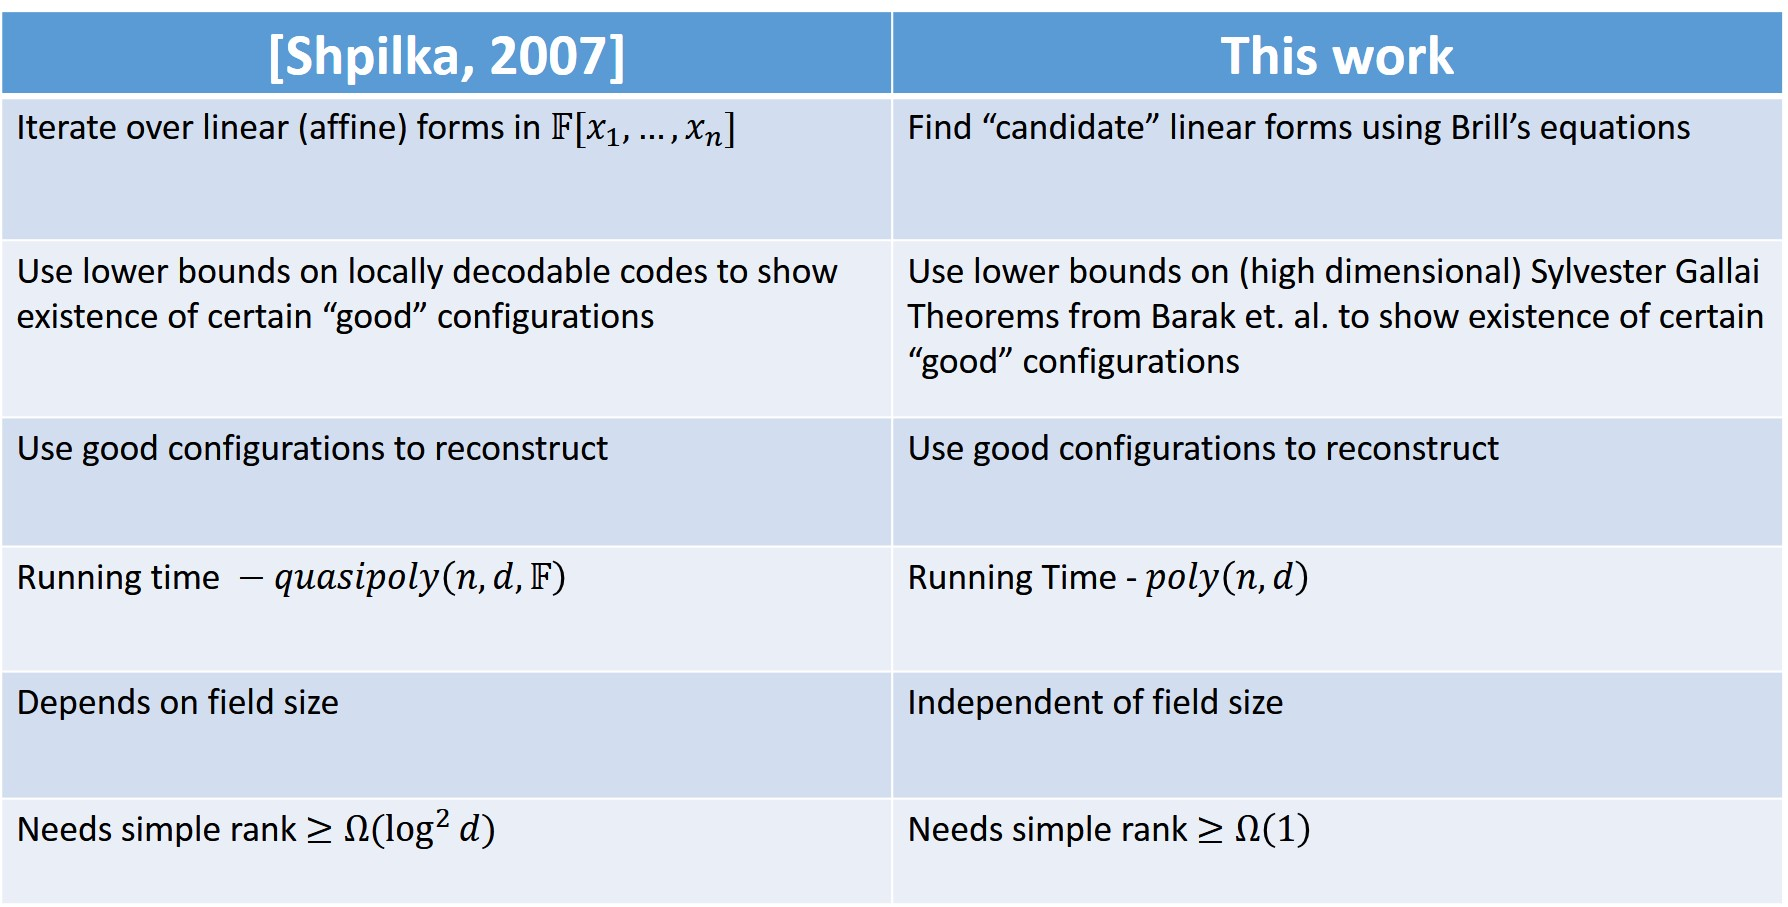
\includegraphics[width = 6in, height=3in]{comparison.jpg}




A further extension of this result was given in \cite{KarShp09}. They derandomized the above algorithm and gave 
generalizations to \emph{"generalized"} $\Sigma\Pi\Sigma(k)$ circuits. The output of their algorithm is not exactly a $\Sigma\Pi\Sigma(k)$ circuit
but something close enough. We do not state the theorem here and instead redirect the reader to their 
paper. Please see Theorem \rom{1} in \cite{KarShp09}.


\begin{theorem}[Rank-bounds for identically zero $\Sigma\Pi\Sigma(k)$ circuits over $\F$ ($\Q,\R,\C$), 
combination of theorem $1.4$ in \cite{SS10} and 
theorem \cite{DSW12}]\label{theorem:rankboundtheorem}

Let $C$ be a simple and minimal $\Sigma\Pi\Sigma(k)$ circuit in $n$ variables over $\F$ such that it computes the identically zero
polynomial, then $srank(C) < R(k,\F)$, where $R(k,\F)$ just depends on $k$. In particular, when $k$ is a constant $srank(C) = O(1)$.

\end{theorem}


\section{Homogenization of $\Sigma\Pi\Sigma(2)$ circuits}\label{section:homogenization}
Let $f(\B{x}) = M_1+M_2$ be a polynomial such that $M_1,M_2$ are products of affine forms in variables $x_1,\ldots,x_n$. We will describe
a homogenous polynomial $f^{hom}(x_1,\ldots,x_n,z) \in \F[x_1,\ldots,x_n,z]$ associated to $f(\B{x})$ such that the reconstruction problem 
for $f^{hom}$ solves the reconstruction problem for $f$. Assume the degree of $f$ is $d$ and denote by $f^d(\B{x})$ the degree $d$ homogeneous
component of $f$. From lemma $2.1$ in \cite{Dvir2014} we see that in $poly(n,d)$ time we can get black-box access to the homogeneous component $f^d$, 
given black-box access to $f$. Define
\[
 f^{hom}(x_1,\ldots,x_n,z) = \begin{cases}
     z^df(\frac{x_1}{z},\ldots,\frac{x_n}{z})  &  z\neq 0 \\
       f^d(x_1,\ldots,x_n) & z=0 \\
   \end{cases}
\] 
 
\begin{lemma}
 Given a black-box $\CB$ for $f$ and the parameters n,d, in time $poly(n,d)$ we can simulate a black-box $\CB^{hom}$ for $f^{hom}$.
\end{lemma}
\begin{proof}
 Proof is straight-forward. We describe how to query $\CB^{hom}$ at point $(x_1,\ldots,x_n,z)$. 
 If $z\neq 0$, we query $\CB$ at $(\frac{x_1}{z},\ldots,\frac{x_n}{z})$ and then multiply the result with $z^d$.
 If $z = 0$, lemma $2.1$ in \cite{Dvir2014} computes $\CB^{hom}$ at the point $(x_1,\ldots,x_n,z)$ by computing $f^d(x_1,\ldots,x_n)$. 
\end{proof}

Now suppose we have reconstructed $f^{hom}(x_1,\ldots,x_n,z)$, we can reconstruct $f(x_1,\ldots,x_n)$ by
substituting $z=1$ in the circuit for $f^{hom}$.









\chapter{Some Definitions, Main Tools and Techniques}\label{chapter:sps2definitions}


\section{Introduction}\label{section:sps2circuit}
Let $\F$ be a field and $\B{x} = (x_1,\ldots,x_n)$ be a tuple of variables. 
\begin{definition}\label{definition:sps2circuit}
An arithmetic circuit $C$ is called a $\Sigma\Pi\Sigma(2)$ circuit if it computes a polynomial $C(\B{x})\in \F[\B{x}]$ of the form:
\[
C(\B{x}) = M_1 + M_2.
\]
where $M_1,M_2$ are products of linear forms. In this case we call $C(\B{x})$ a $\Sigma\Pi\Sigma(2)$ polynomial.
\end{definition}


\begin{definition}[Some associated definitions and observations]\label{definition:definitionsandobservations} We define some 
other associated polynomials, multi-sets and make certain observations (note that the polynomials are defined up to scalar multiplication).

\begin{itemize}
\renewcommand\labelitemi{--}
\item We define $Gcd(C)\in \F[\B{x}]$, to be the $g.c.d.$ (greatest common divisor) of the two products 
$M_1,M_2$ i.e. $Gcd(C) = gcd(M_1,M_2)$. We write $M_1 = Gcd(C)R$ and $M_2 = Gcd(C)B$ where $R,B$ are products of linear forms
and $gcd(R,B)=1$. We can factorize the polynomial $C(\B{x})$ as
 \begin{equation} \label{equation:factorize}
C(\B{x}) = Gcd(C)(R+B).
\end{equation}
If $Gcd(C)=1$, then we say that the circuit $C$ is \emph{"simple"}.
\item $Sim(C) = R+B$, is called the \emph{"simple part"} of circuit $C$, since the two products $R,B$ don't have 
any   common factors.

\item Let $\PP(R), \PP(B),\PP(Gcd(C))$ denote the multi-sets of   projective linear factors of $R,B,Gcd(C)$ respectively. 

\item It is important to note that $Sim(C)$ itself might have more   linear factors. As an example consider the polynomial $(x+y_1)\ldots (x+y_n) - y_1\ldots y_n$,
where $x,y_1,\ldots,y_n$ are variables. This polynomial is divisible by $x$ but $x$ does not divide any of the two products 
$(x+y_1)\ldots (x+y_n)$ and $y_1\ldots y_n$.

\item We define $Int(C)$ as the product of all   linear factors (up to scalar multiplication) of $Sim(C)$ and call it \emph{"internal factors"}. 
Similarly $Res(C)$ (called \emph{"residual factors"})
is defined to be the product (again up to scalar multiplication) of all non-linear irreducible factors of $Sim(C)$.
\item \emph{"Simple rank"} of the circuit $C$ denoted by $srank(C)$ is defined as dimension of the multi-set $\PP(R)\cup\PP(B)$ (see \ref{defn:dimension}
for definition of dimension). 

\end{itemize} 
 
 
\end{definition}


For any multi-sets $\MS,\MT$ of projective linear forms in the projective space $\PP(V)$ we define a 
set of projective linear forms called the \emph{"intersection set"}. This set contains forms in
$\MS\cup \MT$ along with the forms which lie at the intersection of distinct lines connecting $\MS$ and $\MT$. Formally:

\begin{definition}[Intersection set]\label{definition:intersectionset}
 Let $\MS,\MT\subset \PP(V)$ be two multi-sets. The \emph{"intersection set"}, $\MI(\MS,\MT)$ comprises of the following:
 \begin{enumerate}
  \item All distinct forms in $\MS,\MT$.
  \item Intersection of distinct lines $\vec L_1 = fl(s,t)$ and $\vec L_2 = fl(s^\prime,t^\prime)$ where $s,s^\prime\in \MS$ and $t,t^\prime\in \MT$. 
 \end{enumerate}
\end{definition}

\begin{note}
It's easy to see that $|\MI(\MS,\MT)|\leq |\MS|^2 |\MT|^2$.
\end{note}

In our application we will use $\MS=\PP(R)$ and $\MT=\PP(B)$. But first, let's prove a straight-forward lemma about 
multi-sets $\PP(R),\PP(B),\PP(Int(C))$:
\begin{lemma}\label{lemma:internalandgates}
The following are true:
\[
 \PP(R)\cap \PP(Int(C)) = \phi, \hspace{2em} \PP(B)\cap \PP(Int(C))=\phi
\]
\end{lemma}
\begin{proof}
 The proofs are similar so we just show one of them. Let $p\in \PP(Int(C))$. Since $Sim(C) = Int(C)Res(C)$, by restricting to $ker(p)$ 
 we see that
 \[
  R_{|_{ker(p)}} + B_{|_{ker(p)}}= 0\Rightarrow R_{|_{ker(p)}} = -B_{|_{ker(p)}}.
 \]
 If $p\in \PP(R)$ then clearly $R_{|_{ker(p)}}=0$ and thus $B_{|_{ker(p)}}=0$ implying that $p\in \PP(B)$. Therefore $p$ divides both $R,B$ but
 $gcd(R,B)= 1$,  a contradiction. 
\end{proof}





\section{Uniqueness of $\Sigma\Pi\Sigma(2)$ Structure}\label{section:uniqueness}
Note that we defined a quantity called $srank(C)$ in definition \ref{defn:simplerank} (and last part of 
definition \ref{definition:definitionsandobservations}). 
It has been studied very extensively in the last decade and a number of efficient algorithms
for polynomial identity testing have been devised by proving clever bounds on it. 
See theorem 1.5 and 1.7 in \cite{SS10} for details. 

In this section we will show that high simple rank of a $\Sigma\Pi\Sigma(2)$ circuit implies unique circuit representation. 
Based on the underlying field
we will have different values for \emph{"high"}. It's captured by the function $R(k,\F)$ mentioned in theorem 
\ref{theorem:rankboundtheorem}.


\begin{theorem}[ Follows from Corollary $7$ in \cite{Shpilka07}]\label{theorem:uniqueness}
 Let $C$ be a $\Sigma\Pi\Sigma(2)$ circuit computing the polynomial $C(\B{x})$ such that $srank(C) > R(4,\F)$, 
 then the circuit $C$ is (essentially) the unique
 $\Sigma\Pi\Sigma(2)$ circuit computing $C(\B{x})$.
\end{theorem}
\emph{Proof.} Using equation \ref{equation:factorize} in definition \ref{definition:definitionsandobservations}, 
write $C(\B{x}) = Gcd(C)(R+B)$. Let $C^\prime$ be another $\Sigma\Pi\Sigma(2)$ circuit 
also computing $C(\B{x})$. Therefore $C(\B{x})$ also has the form $Gcd(C^\prime)(R^\prime + B^\prime ) \Rightarrow$ 
\[
 Gcd(C)(R + B ) -
 Gcd(C^\prime)(R^\prime + B^\prime) = 0
\]

Note that $Gcd(C),Gcd(C^\prime)$ are products of linear forms. We can remove their common factors in the above identity i.e.
let $\B{G} = gcd(Gcd(C),Gcd(C^\prime))$
and let $Gcd(C) = \B{G} H, Gcd(C^\prime) = \B{G}H^\prime$ with $gcd(H,H^\prime)=1$ giving the identity:
\[
 HR + HB - H^\prime R^\prime - H^\prime B^\prime = 0
\]
The polynomial $HR + HB - H^\prime R^\prime - H^\prime B^\prime$ clearly has a $\Sigma\Pi\Sigma(4)$ circuit. It's easy to check that
$gcd(HR,HB, H^\prime R^\prime, H^\prime B^\prime) = 1$. If not then there exists a   linear form $l$ dividing each of the four
polynomials $HR,HB, H^\prime R^\prime,H^\prime B^\prime$. In particular $l$ divides $HR \Rightarrow l$ divides $H$ or $l$ divides $R$.
\begin{itemize}
\item If $l$ divides $H$
then it cannot divide $H^\prime$ ($H,H^\prime$ are co-prime). Therefore it divides both $R^\prime$ and $B^\prime$ which is not possible as they
are co-prime.
\item If $l$ divides $R$ then $l$ does not divide $B$ as $R,B$ are co-prime. $l$ divides $HB$ $\Rightarrow l$ divides $H$ 
which is not possible as was just shown.
\end{itemize}

  So we have a simple $\Sigma\Pi\Sigma(4)$
circuit which is identically $0$. If this is also minimal then by theorem \ref{theorem:rankboundtheorem} simple rank of this circuit 
is $\leq R(4,\F)$ by \cite{SS10} . But that
is not true since $srank(C) >R(4,\F)$. Therefore it's not minimal i.e. some two gates sum to $0$. Going through the several cases we get
either
\[
(HR,HB) = (H^\prime R^\prime, H^\prime B^\prime) \Rightarrow (Gcd(C)R,Gcd(C)B) = (Gcd(C^\prime) R^\prime, Gcd(C^\prime) B^\prime)
\]
or
\[
(HR,HB) = (H^\prime B^\prime, H^\prime R^\prime) \Rightarrow (Gcd(C)R,Gcd(C)B) = (Gcd(C^\prime) B^\prime, Gcd(C^\prime) R^\prime).
\]
Both of these mean  that the circuit $C$ was unique (up to relabeling the multiplication gates).
\qed




\section{Factoring forms of a polynomial}\label{section:factorsps2}


\begin{definition}\label{definition:factoringform}
 Let $f(\B{x})\in \F[\B{x}]$ be a polynomial. We say that a projective linear form $p$ is a \emph{factoring form} for 
 $f(\B{x})$ if $f(\B{x})_{|_{ker(p)}}$  
 is a non-zero product of linear forms in the ring $\F[x_1,\ldots,x_{i-1},x_{i+1},\ldots,x_n]$. See definition \ref{defn:kernel}
 for definition of restriction to $ker(p)$.
 
 The set of factoring forms for a polynomial $f(\B{x})$ will be denoted
 by $\MP(f)$.
\end{definition}

 We will now investigate
properties of factoring forms for polynomials associated with $\Sigma\Pi\Sigma(2)$ polynomials. 


\subsection{Factoring forms for $\Sigma\Pi\Sigma(2)$ polynomials}\label{subsection:factorsps2}

Recall that $Sim(C) = R + B$ with $gcd(R,B)=1$. Let $p\in \PP(R)$ be a projective linear factor of $R$. We easily see that
$Sim(C)_{|_{ker(p)}} = B_{|_{ker(p)}} \neq 0$ (since $gcd(R,B)=1$). $B_{|_{ker(p)}}$ is a non-zero product of linear forms
since $B$ was a product of linear forms, implying that $p$ is a factoring form for $Sim(C)$. Therefore forms in $\PP(R)$
(similarly $\PP(B)$) are factoring forms for $Sim(C)$ and thus belong to $\MP(Sim(C))$. 

This gives us motivation to compute $\MP(Sim(C))$ as
an approach to finding the products $R,B$. However
there is a problem. We don't have access to $Sim(C)$. This problem can be circumvented by using  
$Res(C)$ (defined as residual factors in definition \ref{definition:definitionsandobservations}) instead. 
We later discuss how to get black-box access to $Res(C)$.

In the next theorem we will discuss properties of the set of \emph{factoring forms} of $Res(C)$.
This set turns out to be a subset of the \emph{intersection set} $\MI(\PP(R),\PP(B))$ (for definition of intersection
set see definition \ref{definition:intersectionset}).


\begin{theorem}\label{theorem:candidatestructure}
 Let $C$ be a $\Sigma\Pi\Sigma(2)$ circuit computing the polynomial $C(\B{x})$. Every form $p\in \PP(R)\cup\PP(B)$ belongs to the set of 
 factoring forms $\MP(Res(C))$. Further if we  assume that $srank(C) > R(3,\F)+2$, then : 
\[
 \MP(Res(C))\subset \MI(\PP(R),\PP(B))
\]
i.e. the factoring forms are either forms in $\PP(R),\PP(B)$ or lie at intersections of distinct lines joining
forms in $\PP(R)$ with forms in $\PP(B)$. 
\end{theorem}

\begin{proof}
 
Let $p$ be a factoring form for $Res(C)$.
Recall the definition of internal factors $Int(C)$ from definition \ref{definition:definitionsandobservations}. On restricting to $ker(p)$ we get
(see definition \ref{defn:kernel})
\begin{equation}\label{equation:simple}
 R_{|_{ker(p)}} + B_{|_{ker(p)}} - Int(C)_{|_{ker(p)}} Res(C)_{|_{ker(p)}} = 0
\end{equation}

$p$ being a factoring form for $Res(C)$ implies that $Res(C)_{|_{ker(p)}}$ is a non-zero product of linear forms.  
This gives us an identically
zero $\Sigma\Pi\Sigma(3)$ polynomial $R_{|_{ker(p)}} + B_{|_{ker(p)}} - Int(C)_{|_{ker(p)}} Res(C)_{|_{ker(p)}} = 0$. 

Let's first pull out the g.c.d. $G$ of the three products (multiplication gates) and define
\[
GR^\prime = R_{|_{ker(p)}}, \hspace{2em} GB^\prime = B_{|_{ker(p)}}, \hspace{2em} GF^\prime = Int(C)_{|_{ker(p)}}Res(C)_{|_{ker(p)}}.
\]
with $gcd(R^\prime,B^\prime,F^\prime)=1$. We have two cases:
\begin{enumerate}
 \item \textbf{Case 1 :} \underline{Set of   linear factors of $G$ has dimension more than one :} 
 Since $G$ divides $R_{|_{ker(p)}}$ and $B_{|_{ker(p)}}$, let's assume
 ${R_1}_{|_{ker(p)}} ( \sim {B_1}_{|_{ker(p)}})$ and ${R_2}_{|_{ker(p)}} (\sim {B_2}_{|_{ker(p)}})$ are two 
 linearly independent linear factors of $G$  where
 $R_1,R_2$ divides $R$ and $B_1,B_2$ divides $B$. So we see that $p$ lies on lines 
 $\vec L_1 = fl([R_1],[B_1])$ and $\vec L_2 = fl([R_2],[B_2])$ (recall that $[R_i],[B_i]$ are projectivizations of $R_i,B_i$
 respectively, see definition \ref{defn:projectivization}). Linear independence of  
 ${R_1}_{|_{ker(p)}}, {R_2}_{|_{ker(p)}}$ implies that the lines are distinct. Therefore $p \in \MI(\MR,\MB)$.

 \item \textbf{Case 2:} \underline{Set of   linear factors of $G$ is one dimensional :} 
 Note that we assumed that $srank(C) \geq R(3,\F) + 2 \Rightarrow$ dimension of the linear factors of $R,B$ is 
 greater than $R(3,\F)+2$. Therefore on restricting to the hyperplane the dimension goes down at most by one. That is
 dimension of linear factors of $R_{|_{ker(p)}}, B_{|_{ker(p)}}$ is greater than $R(3,\F)+2-1$. 
 By the assumption in this case we will get that dimension of linear factors of
 $R^\prime,B^\prime$ is greater than $R(3,\F)+2-1-1
 =R(3,\F)$. On simplification (i.e. dividing equation \ref{equation:simple} by $G$) we obtain an 
 identically zero $\Sigma\Pi\Sigma(3)$ polynomial :
\[
 R^\prime + B^\prime - F^\prime = 0.
 \]
 The identically zero $\Sigma\Pi\Sigma(3)$ circuit computing the above polynomial is simple (i.e. the product gates are co-prime) and has 
 \emph{"simple rank"} $\geq R(3,\F)$. Therefore by theorem \ref{theorem:rankboundtheorem} it cannot be minimal.
 Thus two of the products (multiplication
 gates) $R^\prime,B^\prime,F^\prime$ must sum to zero $\Rightarrow$ one of $R^\prime,B^\prime,F^\prime$ is zero.
 \begin{itemize}
  \item If $R^\prime =\frac{R_{|_{ker(p)}}}{G} = 0$, or $B^\prime =\frac{B_{|_{ker(p)}}}{G} = 0$ then $p$ divides 
  $R$ or $B$ and thus $p\in \PP(R)\cup\PP(B)\subset \MI(\PP(R),\PP(B))$.
 \item If $F^\prime=0$ then $R^\prime+B^\prime=0 \Rightarrow R^\prime = -B^\prime$. 
 We know that dimension of linear factors of $R^\prime,B^\prime$ is greater than $R(3,\F)>2$ (if not then we can just re-define $R(3,\F) = 
 max(R(3,\F),3)$).  
 So exactly like case $1$ above we can find   projective linear forms $R_1,R_2$ dividing $R$ and $B_1,B_2$ dividing $B$ such that $p$ lies on 
 distinct lines $fl(R_i,B_i), i\in [2]$ further implying $p\in \MI(\PP(R),\PP(B))$.
 \end{itemize}

 \end{enumerate}


\end{proof}
The next lemma will be very crucial in the reconstruction process. It states that if we have enough projective linear forms from $\PP(R)$, then
every factoring form connects one of them to some projective linear form in $\PP(B)$. We call this the matching lemma. Proof is exactly like the 
last theorem but we still write it for completion.

\begin{lemma}[Matching lemma]\label{lemma:matchinglemma}
 Fix $k = R(3,\F) +2$. Let $[R_1],\ldots,[R_k]$ be independent projective linear forms in $\PP(R)$ and $p$ be any factoring form in 
 $\MP(Res(C))$ but not in $\PP(R)\cup
 \PP(B)$. Then there
 exists $[R_i], i\in [k]$ and $[B_i]\in \PP(B)$ such that $p$ lies on the line $fl([R_i],[B_i])$.
\end{lemma}
\begin{proof}
Assume the converse i.e. for some factoring form $p$ there does not exists such $R_i,B_i$. Exactly like the previous theorem we obtain
 \[
 R_{|_{ker(p)}} + B_{|_{ker(p)}} - Int(C)_{|_{ker(p)}} Res(C)_{|_{ker(p)}} = 0
\]
 
 and then define $G,R^\prime,B^\prime,F^\prime$ such that
 \[
GR^\prime = R_{|_{ker(p)}}, \hspace{2em} GB^\prime = B_{|_{ker(p)}}, \hspace{2em} GF^\prime = Int(C)_{|_{ker(p)}}Res(C)_{|_{ker(p)}}.
\]
with $gcd(R^\prime,B^\prime,F^\prime)=1$. Following the previous proof we have the identity
\[
 R^\prime+B^\prime-F^\prime=0
\]
If for any $R_i, i\in [k]$, the restriction ${R_i}_{|_{ker(p)}}$ divides $G$, then exactly like the previous proof there is a 
  projective linear form $[B_i]$ dividing $B$ such that $p\in fl([R_i],[B_i])$ and we are done.
  
So assume that all ${R_i}_{|_{ker(p)}}, i\in [k]$ divide $R^\prime$. We know that the restrictions $\{{R_i}_{|_{ker(p)}} : i\in [k]\}$
have dimension equal to $k-1 > R(3,\F)$ implying that simple rank of the $\Sigma\Pi\Sigma(3)$ circuit 
$R^\prime+B^\prime-F^\prime $ is greater than $R(3,\F)$ $\Rightarrow$ (exactly like last proof) it cannot be minimal, 
otherwise it violates rank bound for identically zero polynomials in theorem \ref{theorem:rankboundtheorem}. So like the previous proof some
product gate is zero. $p\notin\PP(R)\cup \PP(B)$ implies $R^\prime,B^\prime$ are non-zero $\Rightarrow F^\prime=0 \Rightarrow R^\prime = -B^\prime \neq 0$.
Hence there exists projective linear form $[B_1]$ dividing $B$ such that ${B_1}_{|_{ker(p)}} \sim {R_1}_{|_{ker(p)}}$ and 
$p$ lies on line $fl([R_1],[B_1])$. 

\end{proof}

\section{ Good forms and reconstructed multi-set}\label{section:goodforms}

In this section we explain the main object that accomplishes the goal of reconstruction in chapter \ref{section:steptwo}.
 Later in chapter \ref{section:steptwo}, we will show that these objects exist and apply them to reconstruct our multi-sets
$\PP(M_1),\PP(M_2)$.


\begin{definition} [Good form] \label{defn:goodform}
Let $p$ be a projective linear form in $\PP(V)$, $\MS, \MT$ be multi-sets in $\PP(V)$. We say that $p$ is a
\emph{"good form"} for $(\MS,\MT)$ if there exists $s \in \MS, t\in \MT$ such that :
 \begin{enumerate}
 \item \label{form1}$p,s,t$ are pairwise distinct.
 \item \label{form2}The forms $p,s,t$ are not collinear.
 \item \label{form3}The plane $\Psi_{p,s,t} = fl(p,s,t)$ intersects $\MT$ only along the line $fl(p,t)$.
 \end{enumerate}

 We collect all $t\in \MT$ for which there exists some $s\in \MS$ such that $p,s,t$ satisfy the above requirements. This multi-set
 will be very special for us. We'll be able to reconstruct it. Let's give it a name.


 \begin{definition}\label{defn:reconstructedset}
 Suppose $p$ is a \emph{"good form"} for $(\MS,\MT)$ we define the \emph{"reconstructed multi-set"} $\MT_p\subset \MT$ as
 \[
 \MT_p = \{\tilde t\in \MT : \exists s \in \MS : (p,s,t)\text{ satisfy bullets \ref{form1}, \ref{form2} and \ref{form3} 
 in definition \ref{defn:goodform}}\}
 \]
 \end{definition}



\end{definition}

Later on we will show how we can reconstruct multi-sets when a good form is given. But first we describe an example of a good form.
This example demonstrates two very important applications of good forms in chapter \ref{section:steptwo}. Here is a lemma.

\begin{lemma}\label{lemma:goodformsapplication}
 Suppose $p,s \in \PP(V)$ are projective linear forms and $\MT$ be a multi-set of projective linear forms.
 Assume
 \begin{itemize}
   \renewcommand\labelitemi{--}
  \item $p\neq s$ and $fl(p,s)\cap fl(\MT) = \phi$.
 \end{itemize}
Then $p$ is a good form for $(\{s\},\MT)$ and the \emph{"reconstructed multi-set"} is $\MT_{p} = \MT.$ 
\end{lemma}
\begin{proof}
 The proof is particularly simple. Consider any $t\in \MT$. 
 \begin{itemize}
  \item Since $p\neq s$ and $fl(p,s)\cap fl(\MT) = \phi$ we get that $p,s,t$ are pairwise distinct and independent. Therefore condition \ref{form1}
  and condition \ref{form2} in definition \ref{defn:goodform} are satisfied.
  \item Consider $\Psi = fl(p,s,t)$. Consider any $t^\prime (\neq t) \in \Psi \cap \MT$. So we may write $t^\prime = \alpha_p p + \alpha_s s + \alpha_t t$,
  with at least one of $\alpha_p,\alpha_s,\alpha_t$ non-zero. If $\alpha_s \neq 0$, then we may re-write the equation as 
  $\alpha_s s + \alpha_p p = t^\prime -\alpha_t t \Rightarrow fl(s,p)\cap fl(t,t^\prime)\neq \phi$ (as $\alpha_s\neq 0$). Therefore
  we arrive at a contradiction to $fl(p,s)\cap fl(\MT) = \phi \Rightarrow \alpha_s = 0\Rightarrow \Psi \cap \MT \subset fl(p,t)$. Therefore
  $p,s,t$ satisfy condition \ref{form3} in definition \ref{defn:goodform}.
 \end{itemize}
Therefore $p$ is a good form for $(\{s\},\MT)$. Also since $t\in \MT$ was arbitrary, bullets \ref{form1},\ref{form2},\ref{form3} in definition 
\ref{defn:goodform} hold for all $t\in \MT$ and thus the reconstructed multi-set in this case is $\MT_{p} = \MT$.
\end{proof}




\begin{lemma}
 Suppose $p \in \PP(V)$ is a "good form" for $(\MS,\MT)$ and let $\MT_p\subset \MT$ be the "reconstructed multi-set".
 Further assume the following
 \begin{enumerate}
  \item The form $p$ and the multi-set $\MS$ are known. Multi-set $\MT$ is unknown.
  \item The multi-set of lines $\ML(p,\MT)$ (see definition \ref{definition:lines}) is known.
  \item For every $s\in \MS$, the multi-set of lines $\ML(s,\MT)$ is known.
 \end{enumerate}
 Then there exists a deterministic algorithm that runs in $poly(|\MS|, |\MT|,n)$ time and reconstructs the multi-set $\MT_p$.
\end{lemma}
\begin{proof}
Let's first give the algorithm and then discuss correctness and time complexity.
\begin{framed}

\begin{algorithm}[H]\label{algorithm:goodformalgo}

Initialize $\tilde\MT_p = \phi$.

\For {each $s (\neq p) \in \MS$}{

Let $\vec L$ be the line $fl(p,s)$.

\For{ each  line $\vec{L}_p$ inside $\ML(p,\MT)\setminus \{\vec L\}$ }{

 Consider the plane $\Psi = fl(\vec L_p,s)$ spanned by line $\vec L_p$ and form $s$.
 
 Find lines in $\ML(p,\MT)$ lying on $\Psi$.
 
 \If { $\vec L_p$ is the only such line  }{
    
    \For{ each line $\vec L_s \in \ML(s, \MT)\setminus \{\vec L\}$, lying on $\Psi$ }{
    
     Let $\tilde t$ be the intersection of lines $\vec L_p$ and $\vec L_s$.
     
     Update $\tilde\MT_p = \tilde\MT_p \cup \{ \tilde t \}$ (note that this is multi-set union).
     
    }

   }

  }
}

Return $\tilde\MT_p$.
\caption{Reconstruction using a Good form}
\end{algorithm}

\end{framed}




\textbf{Correctness Proof - }
We will show below that the set $\tilde\MT_p$ computed by the above algorithm is the same as the "reconstructed multi-set" i.e. $\tilde \MT_p = \MT_p$.

\begin{enumerate}
 \item \textbf{Proof of $\MT_p \subset \tilde\MT_p$ :}  Let $t \in \MT_p$. By the definition of \emph{"reconstructed multi-set"} above, 
 we know that there is an
 $s \in \MS$ such that $(p,s,t)$ satisfy conditions in definition \ref{defn:goodform}. 
 The first for loop will select $s$ at some point of time. Definition \ref{defn:goodform} implies that $fl(p,t)$ does not contain $s$ and so 
 after choosing $s$, the second for loop selects the line $\vec L_p = fl(p,t)$
 at some point of time.
  Since $(p,s,t)$ satisfy conditions of definition
 \ref{defn:goodform}, $\vec L_p$ is the only line from $\ML(p,\MT)$ on the plane $\Psi = fl(p,s,t)$, and so the if condition inside the second for 
 loop will be true. Therefore the algorithm will further choose $\vec L_s = fl(s,t)$ at some point of time. Clearly
 $t$ is the intersection of lines $\vec L_p$ and $\vec L_s$.
 When this happens $t$ gets added to the set $\tilde\MT_p$ implying that $\MT_p \subset \tilde\MT_p$.

 \item \textbf{Proof of $\tilde\MT_p\subset \MT_p$ : } Consider a form $\tilde t \in \tilde\MT_p$. We first show that
 $\tilde t \in \MT$. The algorithm constructs $\tilde t$ as intersection of two lines $\vec L_p \in \ML(p,\MT)$ and
$\vec L_s \in \ML(s,\MT)$ for some $s\in \MS$. Both these lines are different from the line $\vec L = fl(p,s)$. 
Clearly $\vec L_s = fl(s,t)$ for some $t\in \MT$.\\

We show that $\tilde t=t$. Suppose not, then since $\tilde t \in \vec L_s$ and $s\neq \tilde t$ (otherwise $s\in \vec L_p$), we have three distinct forms 
$\{s, \tilde t,  t\}$ on $\vec L_s$.
The line $\vec L_s$ was chosen to be on the plane $\Psi = fl(\vec L_p, s)$. Therefore there are two distinct lines $fl(p,t)$ and $\vec L_p = 
fl(p,\tilde t)$ on this plane $\Psi$. This is a contradiction to the choice of $\vec L_p$, thus $\tilde t = t$.
\begin{itemize}
\item $p,s$ are different by choice of $s$ in the second for loop. $\tilde t$ is intersection of two lines $\vec L_p,\vec L_s$ (different from $\vec L$) and thus $\tilde t$
is different from both $p,s$. Thus condition \ref{form1} in definition \ref{defn:goodform} is satisfied for $(p,s,\tilde t)$.
\item Since $\vec L_p$ was different from the line $\vec L$, we get that $p,s,\tilde t$ are not collinear so condition \ref{form2} in 
definition \ref{defn:goodform} is satisfied for $(p,s,\tilde t)$
\item Let $t\in \MT$ be any projective linear form on the plane
$\Psi = fl(s,\vec L_p) = fl(p,s,\tilde t) = \Psi_{p,s,\tilde t}$ . If $t$ lies on line $\vec L_p = fl(p,\tilde t)$ we are fine. If not then 
$fl(p,t)$ is a line from $\ML(p,\MT)$ different from $\vec L_p$, passing through $p$ and lying on $\Psi$, which is a contradiction to the choice of $\vec L_p$.
Therefore $\psi_{p,s,\tilde t}\cap \MT \subset  fl(p,\tilde t)$ and condition \ref{form3}  in definition \ref{defn:goodform} is satisfied for $(p,s,\tilde t)$.
\end{itemize}
\end{enumerate}
\textbf{Time Complexity :} We examine the nested loop structure. First loop runs $\leq |\MS|$ times. Second loop runs $\leq |\ML(p,\MT)|$ 
times. Inside the second loop finding all lines in $\ML(p,\MT)$ takes $|\ML(p,\MT)| poly(n)$ steps since testing whether a line lies on a plane
in $n$ dimensions can be solved using linear algebra in $poly(n)$ steps. Inner most loop runs $\leq |\ML(s,\MT)|$ times and finding intersection
of lines again takes $poly(n)$ time using linear algebra techniques. It's easy to see that $|\ML(p,\MT)|, |\ML(s,\MT)|$ are both $\leq |\MT|$ and
so overall we take $poly(|\MT|, |\MS|, n)$ time.

So we see that $\MT_p$, the \emph{"reconstructed multi-set"} is actually reconstructed by the above algorithm in $poly(|\MS|, |\MT|, n)$ time.
\end{proof}





















\chapter{Main result and overview} \label{chapter:charzero}
In this chapter we will state our main theorem and also give an outline of the algorithm which the theorem claims. Proof of this theorem
is a combination of results in the next two chapters.
The underlying field for this entire work will be $\F$, a field of characteristic zero. For simplicity we assume it to be $\Q,\R$ or $\C$. 
Our tuple of variables will be denoted by
$\B{x} = (x_1,\ldots,x_n)$. Fix $N_0$ to be large enough constant (see beginning of chapter \ref{section:steptwo} for details). 
Here is the main theorem:

\begin{theorem}\label{theorem:maintheorem2}
Let $C$ be a homogeneous $\Sigma\Pi\Sigma(2)$ circuit computing a degree $d$ polynomial $C(\B{x})$ in $n$ variables $x_1,\ldots,x_n$. 
Assume that black-box access to 
$C$ has been given (along with parameters $n,d$). We give a randomized algorithm that runs in time $poly(n,d)$ and with 
 probability $1-o(1)$ outputs the following:
\begin{itemize}
 \item When $srank(C)$\footnote{This is just the rank of $Sim(C)$.} $\geq N_0$, the output is a $\Sigma\Pi\Sigma(2)$ circuit computing $C(\B{x})$.
%\item When $srank(C) < N_0$, the output is a $\Sigma\Pi\Sigma(k)$ circuit computing $C(\B{x})$ with $k=poly(n,d)$.
 \end{itemize}
\end{theorem}

\section{Overview of the algorithm }

Recall that we are dealing with a $\Sigma\Pi\Sigma(2)$ circuit computing the polynomial:
\[
 C(\B{x}) = M_1(\B{x}) + M_2(\B{x})
\]
where $M_1,M_2$ are products of linear forms. Given black-box access to $C$, we wish to compute $M_1,M_2$. Our algorithm has two
very broad steps :

\subsection{Step \rom{1} - Reconstruct \rom{1}$^{st}$ layer of the circuit}
In this step we try to find a set of linear forms which appear at layer \rom{1} in the circuit $C$. 
These are precisely the linear factors of $M_1,M_2$. We end up reconstructing 
a few extra linear forms and get rid of them afterwards.  At the \rom{1}$^{st}$ layer, we have the following two categories
of linear forms.
\begin{enumerate}
 \item \textbf{Linear forms at layer \rom{1} which divide $C(\B{x})$ - } These are precisely the common linear factors of $M_1,M_2$. 
 Such linear forms definitely
 divide the polynomial $C(\B{x})$.  However these may not be all linear factors of $C(\B{x})$. Consider the polynomial $(x+y_1)\ldots(x+y_n) - y_1\ldots y_n$.
 The linear form $x$ divides the polynomial but does not divide any of the two products $(x+y_1)\ldots(x+y_n)$ and $y_1\ldots y_n$. 
 Instead of computing the set of common linear factors of $M_1,M_2$, we compute the set of all linear factors of $C(\B{x})$. Later on
 during step $2$ of the algorithm, the bad forms get rejected. In order to find all linear factors of $C(\B{x})$, we use the standard black-box factoring
 algorithm of \cite{KalTr90}. The algorithm gives us access to black-boxes for the factors. We convert them into explicit coefficient form
 in algorithm \ref{algorithm:blackboxfactors}.
 
 \item \textbf{Linear forms at layer \rom{1} which don't divide $C(\B{x})$ - } Let's write $M_1 = Gcd(M_1,M_2) R$ and $M_2 = Gcd(M_1,M_2)B$ where $R,B$
 are products of linear forms such that $gcd(R,B)=1$.
 Then the linear forms at layer \rom{1} which don't divide $C(\B{x})$ are precisely the linear factors of $R$ and $B$. 
 We compute a set of size $poly(n,d)$
 such that it contains all distinct linear factors of $R$ and $B$. This is achieved by first making a random invertible transformation in Section
 \ref{section:stepzero} to make sure that our variables $x_1,\ldots,x_n$ become \emph{"random"}. Next in $C(\B{x})$ we set all but 
 constant many variables to zero. The restriction of our polynomial to constant many variables can actually be computed in coefficient 
 form efficiently using the original black-box. 
 
 Now for this restricted polynomial, we find a  set of linear forms which 
 contains the (restricted) linear factors of $R,B$. This is done using brill's equations (see appendix 
 \ref{appendix:brills}) which completely characterize the coefficients of polynomials which split into linear factors. We repeat the whole
 process for different subsets of constant many variables and compute a set containing restricted linear factors of $R,B$ in each case. 
 Finally we describe a method to glue all these sets of restricted linear forms. 
 This gives us a set of linear forms over $x_1,\ldots,x_n$ containing linear factors of $R,B$. The linear forms in this final set has
 certain bad elements (forms which don't divide $R,B$). But these bad forms have certain structure and get rejected during the course 
 of our algorithm.
 
 \item The two multi-sets computed above are then sent to the next part of the algorithm which involves reconstructing 
 the \emph{"wiring"} of the circuit and finding the gates at layer \rom{2}. Along with these sets, as a by-product of algorithm \ref{algorithm:blackboxfactors}
 we also compute a black-box computing the polynomial which is the product of all non-linear irreducible factors of $C(\B{x})$.
 This is also used to reconstruct the gates at layer \rom{2}.
\end{enumerate}


\subsection{Step \rom{2} - Reconstruct \rom{2}$^{nd}$ layer of the circuit}
In this step we use the linear forms and the black-box (computing product of non-linear irreducible 
factors of $C(\B{x})$) computed above and reconstruct the wiring in the graph of our circuit. 

Suppose $r,b$ are linear forms dividing $R,B$ respectively. Using the outputs from step \rom{1}, we can calculate the multi-sets 
\[ \{l\Mod{r} : l\text{ is a linear factor of } M_2  \},\hspace{1em} \{l\Mod{b} : l\text{ is a linear factor of } M_1  \}.
\] 

Viewing the linear forms as points in space, the above multi-sets enable us to find multi-sets of lines going from $r$ to linear factors of $M_2$
and multi-sets of lines going from $b$ to linear factors of $M_1$.

Next we look for non-degenerate planes $\Psi = sp\{r_1,r_2,l\}$ ($sp\{b_1,b_2,l\}$) where $r_1,r_2$ are linear factors of $R$ and
$l$ is a linear factor of $M_2$ (resp. $b_1,b_2$
are linear factors of $B$ and $l$ is a linear factor of $M_1$ ) satisfying the following condition. 
\begin{itemize}
 \item Linear factors of $M_2$ (resp. $M_1$) lying on $\Psi$ only lie on the line $\overrightarrow{r_1,l}$ (resp. $\overrightarrow{b_1,l}$). 
\end{itemize}

We show that if such a configuration exists, then we can reconstruct $l$ along with the multiplicity with which it 
divides $M_2$ (resp. $M_1$) by considering intersections of lines in $\Psi$.
So the whole effort then goes into showing existence of such planes $\Psi$ (and that it can be found efficiently in every iteration
of the algorithm). To do this we use quantitative versions of the Sylvester Gallai theorem given in \cite{BDWY11} and it's improvements 
from \cite{DSW12}. 

During the algorithm one of the problems we encounter is that the set $\MP$ provided by step \rom{1} contains points other than 
linear factors of $R,B$. So we need to make sure that we do not use these \emph{bad points}. We do this by finding structure (see matching lemma, 
\ref{lemma:matchinglemma}) 
in these bad points (due to the way they were
constructed) and use this structure to eliminate them. If we can do this wisely then the reconstruction process goes smoothly. 

Finally, if we have reconstructed all the linear factors for one of the products $M_1,M_2$ we compute an appropriate constant that we need to
multiply to the product of our linear forms (since all linear forms will be obtained up to scalar multiplication). This is done by
using brill's equations again and the algorithm has been explained in subsection \ref{subsection:othergate}. This will be the last step of
all our reconstruction algorithms in step \rom{2}.

Once we have done the above our reconstruction is complete. For technical reasons we work with projective linear forms instead
of linear forms in the entire discussion above. This is done to give better exposition by avoiding certain trivial
technicalities that appear when a linear form is
known only up to scalar multiplication.


%\section{Overview of the algorithm when $srank(C)$ is low }








\chapter{Step One : Reconstruct the \rom{1}$^{\text{st}}$ Layer of $C$ }\label{section:stepone}

\section{Introduction}


Recall that we have access to a black-box $\CB$ for a $\Sigma\Pi\Sigma(2)$ circuit $C$ computing the polynomial 
$C(\B{x}) = M_1 + M_2 = Gcd(C) (R+B) = Gcd(C)Int(C)Res(C)$ (see definition \ref{definition:definitionsandobservations}). 
In this chapter we wish to use $\CB$ and compute all the
  projective linear forms corresponding to linear forms computed at the first layer in circuit $C$. 

On looking closely we can see that the outputs at layer \rom{1} are just (scalar multiples of) the linear factors of $Gcd(C) = gcd(M_1,M_2)$ and polynomials
$R, B$. 
Thus our main objective for this chapter is to find the multi-set of projective linear forms 
$\PP(Gcd(C))\cup\PP(R)\cup \PP(B)$, where the union is a multi-set union. We will not be constructing this multi-set exactly but something 
close enough.

In this section we give algorithms to compute the following:
\begin{enumerate}
\item The multi-set $\PP(Gcd(C)Int(C))$ which is the multi-set of  projective linear factors of 
$C(\B{x})$. By abuse of notation we say that a projective linear form divides a polynomial whenever a corresponding 
linear form divides the polynomial. 

\item A set $\MP\subset \PP(V)$ of   projective linear forms containing (distinct) projective linear forms from 
$\PP(R)$ and $\PP(B)$. We wish to emphasize that this set does not give us information about multiplicities
of forms in their respective sets $\PP(R)/\PP(B)$. For that we develop methods in chapter \ref{section:steptwo}. 
The set $\MP$ that we compute here has size $poly(d)$ where $d$ is the degree of $C(\B{x})$.
\end{enumerate}






The first part of the theorem i.e. computing $\PP(Gcd(C)Int(C))$ has already been done in algorithm \ref{algorithm:blackboxfactors} of 
appendix \ref{appendix:blackboxfactors} using kaltofen's black-box factoring algorithm from \cite{KalTr90}. It also gives
us a black-box $\CB_{Res}$ computing $Res(C)$. We just invoke the algorithm here and move on to solve the second part. Thus our goal becomes:


 \textbf{Goal of this Section. } Given a $\Sigma\Pi\Sigma(2)$ circuit $C$ as a black-box,
 efficiently compute a set of   projective linear forms $\MP$  such that:
 \begin{itemize}
  \renewcommand\labelitemi{--}
  \item $p \in \PP(R)\cup \PP(B) \Rightarrow p\in \MP, \hspace{0.25em}\text{ and }\hspace{1em}|\MP| = poly(d)$.
 \end{itemize}

 
We achieve this goal by computing the set of \emph{"factoring forms"} 
(see definition \ref{definition:factoringform}) for the polynomial $Res(C)$ i.e.
\[
\MP \defeq \MP(Res(C)).
\]
As we mentioned before solving the first part using algorithm \ref{algorithm:blackboxfactors} already gave us access to a black-box $\CB_{Res}$
computing $Res(C)$. The reasons for choosing this set $\MP$ are mentioned below.

\begin{note}[From theorem \ref{theorem:candidatestructure}]\label{note:candidatestructure}
 For any $\Sigma\Pi\Sigma(2)$ circuit $C$ computing polynomial \[C(\B{x}) = Gcd(C)(R+B) = Gcd(C)Int(C)Res(C)\]
 we have:
 \begin{itemize}
 \item Any $p\in \PP(R)\cup \PP(B)$ belongs to $\MP(Res(C))$, i.e. $p$ is a \emph{"factoring form"} for the polynomial
 $Res(C)$.

 \item  if $srank(C)$ is high enough ($\geq R(3,\F)+2$), then $\MP(Res(C))\subset \MI(\PP(R),\PP(B))$ and therefore 
 $|\MP(Res(C))|\leq d^4.$

 \end{itemize}
\end{note}
So this set satisfies both properties we wanted in $\MP$. From now onwards we set $\MP \defeq \MP(Res(C))$ and try to
compute it using the black-box.



Let's summarize our result in the following theorem:

\begin{theorem}\label{theorem:stepone}

Let $C$ be a homogeneous $\Sigma\Pi\Sigma(2)$ circuit computing a degree $d$ polynomial $C(\B{x})$ in $n$ variables $x_1,\ldots,x_n$. 
Assume that black-box access to 
$C$ has been given (along with parameters $n,d$).
Further assume that $srank(C)>  max(R(3,\F)+2,R(4,\F))$. There exists a randomized algorithm that runs in time 
 $poly(n,d)$ and  outputs two multi-sets $\MF$ and $\MP$ of projective linear forms such that
 \[
  Pr[ \MF = \PP(Gcd(C)Int(C))\hspace{0.5em} \text{ and }\hspace{0.5em} \MP = \MP(Res(C)) ]\geq 1-o(1) 
 \]
\end{theorem}



To compute this set $\MP$ we follow a standard \emph{"restrict and lift"} technique. The broad idea is:
\begin{enumerate}
 \item \textbf{Restriction Step - } Restrict $C(\B{x})$ to a number of \emph{"random"} low dimensional subspaces of $\F^n$ i.e. set
 many of the variables ( they are \emph{"random"} by the application of a random transformation on the inputs, see section \ref{section:stepzero}) to zero.
 Then using the restricted polynomial we compute sets $\MP_i$ which are (or at least contain) restrictions of $\MP$. These sets $\MP_i$
 can be computed by solving a system of polynomial equations.
 \item \textbf{ Lifting Step - }Once we have the $\MP_i$'s we glue them together. 
 This gives us a set containing $\MP$, since restrictions of forms in $\MP$ are definitely glued. Then we prune this set to throw 
 away the bad forms using the definition of $\MP$ i.e. all forms in $\MP$ are factoring forms for $Res(C)$. The random subspace is very
 important since it makes sure that we glue whatever is needed and we don't take too much time gluing. In short it introduces
 a lot of non-degeneracy among the restrictions.
\end{enumerate}

\section{Random Transformation}\label{section:stepzero}
Before doing any computation with the input black-box $\CB_{in}$, we \emph{"apply"} a random transformation $\tilde\Omega$ to it. 
This has been explained in great detail in appendix \ref{appendix:randomtransform}.

$\tilde \Omega$ is constructed with the help of an $n\times n$ matrix
$\Omega = (\Omega_{i,j})$, where each entry is chosen uniformly randomly and independently from the a set $S\subset \F$. On the set
$\{x_1,\ldots,x_n\}$, $\tilde\Omega$ maps $x_i\mapsto (\Omega\hspace{0.25em} \B{x})_i$ ($\B{x}$ is treated as a column vector $(x_1,\ldots,x_n)^T$).
This map is then extended to an algebra homomorphism on $\F[\B{x}]$. When the matrix $\Omega$ is invertible the map $\tilde \Omega$ becomes an isomorphism. 
We proceed only if $\Omega$ is invertible which happens with a high probability 
by lemma \ref{lemma:matrixinvertible} in appendix \ref{appendix:randomtransform}. If it's not invertible we output \emph{"fail"}.

In order to \emph{"apply"} $\tilde \Omega$ to our input black-box $\CB_{in}$, we define a new black-box $\CB$ such that for every $a\in \F^n$,
$\CB(\B{a}) = \CB_{in}(\Omega^{-1}(\B{a}))$.  This just
means that to query the new black-box $\CB$ at point $\B{a}$, we query the old black-box at point $\Omega^{-1}(\B{a})$. If $\CB_{in}$ computed
the polynomial $f(\B{x})$ then $\CB$ computes $\tilde\Omega(f)$.


From now onwards we assume that $\Omega$ is invertible and  $\tilde \Omega$ has already been applied to the input 
black-box $\CB_{in}$. We will work with the new black-box $\CB$ which also represents a $\Sigma\Pi\Sigma(2)$ circuit
$C$ computing polynomial $C(\B{x})$. We use all definitions in chapter \ref{chapter:sps2definitions} for this circuit/polynomial. 


\subsection{Assumption - Independence preserving restrictions of the intersection set }\label{subsection:assumption}
Recall the definition of intersection set in definition \ref{definition:intersectionset}. Using the 
random transformation defined above we have created a new \emph{"random"}
set of variables $x_1,\ldots,x_n$. Applying $\tilde \Omega$ preserves linear independence since it is an algebra isomorphism
and hence a linear isomorphism.
In subsection \ref{subsection:restrict}, we will restrict our polynomial $C(\B{x})$ to certain 
subsets of these variables. While doing this restriction, we want to preserve independence for points in  the intersection set.
If independence is preserved for restriction of points in $\MI(\PP(R),\PP(B))$ then it automatically gets preserved for 
restrictions of points in  multi-sets $\PP(R),\PP(B)$ and the set $\MP$ 
since they are all subsets of $\MI(\PP(R),\PP(B))$. This turns out to be really beneficial for us when we try to \emph{"glue"} the 
restrictions together. 

We first define the subspaces we'll be restricting to. They will be used frequently and so we make a separate definition for them.

\begin{definition}\label{definition:subspaces}
 Define subspaces $W_{r-1} = \{(w_1,\ldots,w_{r-1},0\ldots,0):w_1,\ldots,w_{r-1} \in \F\} \subset \F^n$
and $W_i = \{ (w_1,\ldots,w_{r-1},0,\ldots,0,w_{i},0,\ldots,0) : w_1,\ldots,w_{r-1},w_i\in \F \}\footnote{ \text{The $w_i$ is in the 
$i^{th}$ location.} } \subset \F^n, i\in \{r+1,\ldots,n\}$.
\end{definition}



Restricting a polynomial to $W_{r-1}$ corresponds to plugging $x_r =\ldots = x_n=0$ and restricting it to $W_i$ corresponds to
plugging $x_r = \ldots = x_{i-1} = x_{i+1} = \ldots = x_n=0$. Restriction of any polynomial $f$ to the subspace
$W_i$ will be denoted by $f_{|_{W_i}}$ and that to $W_{r-1}$ will be denoted by $f_{|_{W_{r-1}}}$.

We also define $V_i$ as vector space of linear forms in $x_1,\ldots,x_{r-1},x_i$ and $V_{r-1}$ as the vector
space of linear forms in $x_1,\ldots,x_{r-1}$.

\begin{definition}[Restrictions of points in projective space]\label{defn:restriction}
Let $p\in \PP(V)$ and consider any $l\in V$ such that $p=[l]$. When $l_{|_{W_i}} \neq 0$ (resp. $l_{|_{W_{r-1}}}\neq 0$)
we say $p_{|_{W_i}}$ (resp $p_{|_{W_{r-1}}}$) is defined, 
and define $p_{|_{W_i}}$ (resp $p_{|_{W_{r-1}}}$) as the point $[l_{|_{W_i}}] \in \PP(V_i)$ (resp. $[l_{|_{W_{r-1}}}] \in \PP(V_{r-1})$). 
Otherwise we say  $p_{|_{W_i}}$ (resp $p_{|_{W_{r-1}}}$) is undefined.

It can be seen that when $p_{|_{W_i}}$ (resp $p_{|_{W_{r-1}}}$) is defined, it is in fact well defined (i.e. if we choose $l^\prime$ 
instead of $l$ we get the same points as restrictions).
\end{definition}


\begin{lemma}\label{lemma:intersectionproj}
 Let $r\geq 4$ and consider subspaces defined in definition \ref{definition:subspaces} above. The following hold
 with high probability:
\begin{enumerate}
\item \label{bullet:nonconstantforms} Let $p\in \MI(\PP(R),\PP(B))$ be a point, then 
${p}_{|_{W_i}}$ is defined and belongs to $\PP(V_i)$ (see definition \ref{defn:restriction}).
\item \label{bullet:independence}Let $p_1,\ldots,p_s \in \MI(\PP(R),\PP(B))$, $s\leq r$ be $s$ independent 
points (see definition \ref{defn:dependentpoints}), then ${p_1}_{|_{W_i}},\ldots,{p_s}_{|_{W_i}}$ are defined and are independent 
points in $\PP(V_i)$. 

\item \label{bullet:formslines}Let $p_1,\ldots,p_s \in \MI(\PP(R),\PP(B))$, $s\leq 3$ be $s$ independent points, 
then the restrictions ${p_1}_{|_{W_{r-1}}},\ldots,{p_s}_{|_{W_{r-1}}}$ are defined and are independent points in $\PP(V_{r-1})$.
\end{enumerate}
\end{lemma}

\begin{proof}
 Apply corollary \ref{corr:nondegeneracy} in appendix \ref{appendix:randomtransform} for multi-set $\MI(\PP(R),\PP(B))$. 
 Note that $|\MI(\PP(R),\PP(B))| \leq d^4$, therefore
success probability is $\geq 1-\frac{poly(n,r,d^{4r})}{|S|}$. 
We will assume $|S|>> \Omega(poly(n,r,d^{4r}))$ and make the probability $\geq 1-o(1)$. From now onwards
 we assume that the statements in this lemma are always true i.e. 
our $\Omega$ is always among the good cases. This is done for better exposition.
\end{proof}




\section{Restricting the input polynomial}\label{subsection:restrict}
Let $r\geq 4$ be any integer. Consider the subspaces $W_i$, $i\in \{r+1,\ldots,n\}$ defined in definition \ref{definition:subspaces}.
We restrict\footnote{ This just means plugging $x_r = \ldots = x_{i-1} = x_{i+1} = \ldots =x_n=0$ } 
$C(\B{x})$ to $W_i$ giving:
\[
C(\B{x})_{|_{W_i}} = {M_1}_{|_{W_i}} + {M_2}_{|_{W_i}} 
\]

Clearly this restriction is also a $\Sigma\Pi\Sigma(2)$ polynomial. We denote the above $\Sigma\Pi\Sigma(2)$ 
circuit computing it as $C_{|_{W_i}}$. We can further factorize using definition \ref{definition:definitionsandobservations}.
\[
C(\B{x})_{|_{W_i}} =  Gcd(C_{|_{W_i}})Sim(C_{|_{W_i}}) = 
Gcd(C_{|_{W_i}})Int(C_{|_{W_i}})Res(C_{|_{W_i}}) 
\]


\begin{lemma}\label{lemma:proj}
The following are true (up to multiplication by a scalar):
\begin{enumerate}
% \item \label{bullet:gatesproj} $\PP(R_{|_{W_i}}) = \PP(R)_{|_{W_i}}, \PP(B_{|_{W_i}}) = \PP(B)_{|_{W_i}}$ 
% i.e. forms from $\PP(R),\PP(B)$ remain   on restriction.
 \item \label{bullet:simpleproj} $gcd(R_{|_{W_i}}, B_{|_{W_i}})=1 \Rightarrow Sim(C_{|_{W_i}}) = R_{|_{W_i}} + B_{|_{W_i}}$.
 \item \label{bullet:rankproj} $srank(C_{|_{W_i}}) = min(r, srank(C))$.
\item \label{bullet:residuals}$Res(C_{|_{W_i}}) = Res(C)_{|_{W_i}}$ with high probability.
\end{enumerate}
\end{lemma}

\begin{proof}
The proof is routine and long. See lemma \ref{lemma:projproof} in appendix \ref{appendix:proofsfromchap4}. To not break
continuity we urge the reader to believe the lemma and verify it later.
\end{proof}

\begin{remark}\label{remark:reason}
We make a few remarks:
 \begin{enumerate}
  \item \label{bullet:residualblackbox} Note that we have already computed a black-box $\CB_{Res}$ computing the polynomial $Res(C)$ using 
  algorithm \ref{algorithm:blackboxfactors}
  in appendix \ref{appendix:blackboxfactors}. Part \ref{bullet:residuals} in lemma \ref{lemma:proj} tells us that 
  $Res(C_{|_{W_i}}) = Res(C)_{|_{W_i}}$, and so
  by feeding the black-box $\CB_{Res}$ inputs from $W_i$ we can obtain a black-box for $Res(C_{|_{W_i}})$.
 
 \item Assuming $srank(C)> r = R(3,\F)+2$, in part \ref{bullet:rankproj} of lemma \ref{lemma:proj} we can say that
 $rank(C_{|_{W_j}})=r = R(3,\F)+2$. Then we can use theorem \ref{theorem:candidatestructure} for this circuit and
 obtain $\MP(Res(C_{|_{W_i}}))\subset \MI(R_{|_{W_i}}, B_{|_{W_i}})$. Also part \ref{bullet:simpleproj} of lemma \ref{lemma:proj}
  and theorem \ref{theorem:candidatestructure} together imply that all   projective linear forms in 
  $\PP(R_{|_{W_i}}), \PP(B_{|_{W_i}})$ are in $\MP(Res(C_{|_{W_i}}))$.
\end{enumerate}
Due to these reasons we try to compute $\MP(Res(C_{|_{W_i}}))$ using the black-box for $Res(C_{|_{W_i}})$ described above.
For shorthand we define $\MP_i = \MP(Res(C_{|_{W_i}}))$.

\end{remark}




\section{Computing the sets $\MP_i$. }

To efficiently compute $\MP_i$, we use brill's equations which
completely characterize coefficients of polynomials expressible as product of linear forms. We discuss them in great detail in 
appendix \ref{appendix:brills}.
Let's first give the main result about these equations and then an algorithm to compute the sets $\MP_i$.

The lemma below says that
there exists a family of polynomials $\MF = \{F_1,\ldots,F_m\}$ such that coefficients of all totally decomposable polynomials 
( i.e. product of linear forms)
are given by the variety $\V(\MF)$. Also this family $\MF$ can be computed in $poly(d^r)$ time as shown in appendix \ref{appendix:brills}.

We first compute coefficient representation for $Res(C_{|_{W_i}})$ using part \ref{bullet:residualblackbox} in remark 
\ref{remark:reason} i.e. we do Lagrange interpolation on $Res(C)_{|_{W_i}}$. This can be done by first restricting
the black-box $\CB_{Res}$ to $W_i$ (by feeding inputs only from $W_i$) and then by using $O(d^r)$ points from $W_i$ to
interpolate. Next we consider any   projective linear form in the $r$ variables $x_1,\ldots,x_{r-1},x_i$. Say the coefficient of $x_j$
is non-zero $\Rightarrow$ we may write a linear form corresponding to this projective form  as 
\[x_j -\sum\limits_{k\in I\setminus \{j\}}z_kx_k\] (here $I$ is the set $\{1,\ldots,r-1,i\}$)
and then substitute for $x_j$ in the polynomial $Res(C_{|_{W_i}})$. We collect the coefficients of this polynomial 
as polynomials in the $z_k$'s and use them as input into the variety $\V(\MF)$ described above. The solutions for these
$z_k$'s can then be obtained using any algorithm to compute roots e.g. buchberger's algorithm (\cite{Buc76}). Since $r = \Omega(1)$,
this algorithm works in $poly(d)$ time as explained below.

\begin{lemma}[Brill's equations, See corollary \ref{corollary:brills} in appendix\ref{appendix:brills}]\label{lemma:brills}
 Let $\F=\C$, and $s,d$ be positive integers.
 Define the indexing set
\[
 \Lambda\defeq \{\lambda = (\lambda_1,\ldots,\lambda_s) : \lambda_i\geq 0 \text{ for all } i,
 \sum\limits_{i\in[s]}\lambda_i\leq d\}
 \]
 Define $ t \defeq |\Lambda| = {s+d\choose d}$. We know that $\Lambda$ can be used to index the coefficients of any multivariate polynomial of degree
 $d$ in $s$ variables. For any coefficient vector ${\bf a }= (a_\lambda)_{\lambda\in \Lambda}$ we have the polynomial
 \[
 f_{\bf a}(x_1,\ldots,x_s) = \sum\limits_{\lambda=(\lambda_1,\ldots,\lambda_s) \in \Lambda}a_{\lambda}x_1^{\lambda_1}\ldots x_s^{\lambda_s}
 \]

There exists an explicit set of polynomials $F_1,\ldots,F_m \in \C[y_1,\ldots,y_t]$ with $m=poly(d)$, such that
\[
f_{\bf a}(x_1,\ldots,x_s) \text{ is totally decomposable } \Leftrightarrow F_1(\bf a) = \ldots = F_m(\bf a)=0
\]
Also this set $\{F_1,\ldots,F_m\}$ can be computed in $poly(t,m)$ time.
\end{lemma}

\paragraph{Algorithm. }
Recall that we've already computed a black-box $\CB_{Res}$ for $Res(C)$ using algorithm \ref{algorithm:blackboxfactors}. 
Here is the algorithm to compute $\MP_i, k\in \{r,\ldots,n\}$ using these black-boxes:

\begin{framed}
\begin{algorithm}[H]\label{candidatealgo}
\SetKwData{Left}{left}\SetKwData{This}{this}\SetKwData{Up}{up}
\SetKwInOut{Name}{FunctionName}\SetKwFunction{FindCompress}{FindCompress}
\SetKwInOut{Input}{input}\SetKwInOut{Output}{output}
%\Name{Candidates}
%\Input {Polynomial $Res(C)$ in black-box form}
%\Output {Set $\MP$ of linear hyperplanes}
%\BlankLine

\For{each $i\in \{r,\ldots, n\}$}{

\vspace{0.5em}

  Initialize $\MP_i=\phi$.
  
  Using part \ref{bullet:residualblackbox} in remark \ref{remark:reason} and Lagrange interpolation, compute $Res(C_{|_{W_i}})$ in coefficient form.
 
 \For {each $j\in I = \{1,\ldots,r-1,i\}$}{
 \vspace{0.5em}
 
 Let $\{z_k\}_{k\in I\setminus j}$ be variables.
 
 Substitute $x_j = \sum\limits_{k\in I\setminus \{j\}}z_kx_k$ in $Res(C_{|_{W_i}})$ and compute the coefficient
 polynomials (in  $\{z_k\}_{k\in I\setminus \{j\}}$) corresponding to monomials in the variables $\B{x}$.
 
 Let ${\bf a} $ be the  vector of coefficient polynomials
 calculated above.
 
 Solve polynomial system $\{F_j({\bf a})=0, j\in [m]\}$ in $\C$, using  Buchberger's Algorithm (\cite{Buc76}).
 
 If a solution $(z_k)_{k\in I\setminus \{j\}}$ belongs to $\F^{r-1}$, add the form 
 corresponding form $x_j - \sum\limits_{k\in I\setminus\{j\}z_kx_k}$ as a projective form to the set $\MP_i$.
 
 }
}
 Return the sets $\MP_r,\MP_{r+1},\ldots, \MP_n$.
\vspace{1em}

\caption{Computing sets $\MP_i = \MP(Res(C_{|_{W_i}}))$}
\end{algorithm}
\end{framed}

Note that since the number of solutions were $O(d^4)$, the polynomial system has at most these many solutions and using
Buchberger's algorithm we can find all of them. Now let's look at the time complexity of this algorithm.
\begin{itemize}
\item When we substitute and expand any monomial in $Res(C_{|_{W_i}})$, we spend $ O(d^r)$
time in computing coefficients of all monomials in the $\B{x}$ variables.
\item Buchberger's algorithm takes $O(d^{2^r})$ time (See \cite{Buc76}).
 \end{itemize}
Rest of the steps are $poly(r,d)$ time. So overall we take $O(d^{2^r})$ time. Since $r$ was set to be a constant ( = $R(3,\F)+2$) 
in remark \ref{remark:reason}, the time taken is
$poly(d)$. We will perform this for all $i\in \{r,\ldots,n\}$ and thus in $poly(d,n)$ time we would have computed our all the  sets
$\MP_i = \MP(Res(C_{|_{W_i}}))$. Now it's time to glue them together and compute the candidate set $\MP$.


\section{Gluing $\MP_i$'s to compute $\MP$} \label{subsection:glueback}
We start with the following observation:

\begin{observation}
 Consider   projective linear forms $p_r\in \MP_r$ and $p_i \in \MP_i, i\in \{r+1,\ldots,n\}$ such that for 
 linear forms $l_r = \sum\limits_{j=1}^{r-1} \alpha_jx_j +\alpha_rx_r$, $l_i = \sum\limits_{j=1}^{r-1} \beta_jx_j + \beta_ix_i$ with 
 $p_r = [l_r]$ and $p_i=[l_i]$ and
 \[{l_r}_{|_{W_{r-1}}} \sim {l_i}_{|_{W_{r-1}}} (\neq 0).\]
 Then there exists a linear form $l$ in variables $x_1,\ldots,x_r,x_i$ which is a lift of both forms $l_r$ and $l_i$. This can be seen as follows. Clearly
 there is some $j\in \{1,\ldots,r-1\}$ such that $\alpha_j\neq 0$. Without loss of generality let's assume $j=1$ (note that this also
 implies that $\beta_1\neq 0$), then we define $l$ as
 \[
  l=x_1+\frac{\alpha_2}{\alpha_1}x_2 + \ldots \frac{\alpha_r}{\alpha_1}x_r + \frac{\beta_i}{\beta_1}x_i.
 \]
 and $p=[l]$ can be seen (or defined) to be a lift on $(p_r,p_i)$. Note that by definition \ref{defn:restriction}, instead 
 of saying ${l_r}_{|_{W_{r-1}}} \sim {l_i}_{|_{W_{r-1}}}$ we could have
 said that ${p_r}_{|_{W_{r-1}}}, {p_i}_{|_{W_{r-1}}}$ are defined and are equal points in $\PP(V_{r-1})$. 
\end{observation}



\begin{definition}
 A pair of   projective linear forms $(p_r,p_i) \in \MP_r\times \MP_i$ are called \emph{"gluable"} if
 ${p_r}_{|_{W_{r-1}}}, {p_i}_{|_{W_{r-1}}}$ are defined and are equal points in $\PP(V_{r-1})$.
 \end{definition}


For $p_r\in \MP_r$ our algorithm tries to find $p_i\in \MP_i, i\in \{r+1,\ldots,n\}$ such that $(p_r,p_i)$ are gluable. If we can successfully find such
$p_i$'s for every $i\in \{r+1,\ldots,n\}$ then gluing $p_r$ with all of them gives us a projective linear form $p$ in variables
$x_1,\ldots,x_n$.




For our algorithm to work in polynomial time and
recover $\MP$ using gluing we need to make sure
of two requirement:

\begin{lemma}\label{lemma:requirements}
 The following hold:
 \begin{enumerate}
\item \label{bullet:part1} For every $p\in \MP$ and $i\in \{r,\ldots,n\}$, $p_{|_{W_i}} \in \MP_i$.
 \item \label{bullet:part2} For any $p_r\in \MP_r$, there is at-most one $p_i\in \MP_i, i\in \{r+1,\ldots,n\}$ it can be glued to.
\end{enumerate}
\end{lemma}
\begin{proof}
 For cleaner exposition we move these proofs to appendix \ref{appendix:proofsfromchap4}.
\end{proof}
To not break continuity, we urge the reader to continue reading at this moment and verify the proof later.
Now we are ready to give the gluing algorithm and recover the set $\MP$. Let's summarize it in the following lemma
\begin{lemma}
 Given sets $\MP_i$ and black-box $\CB_{Res}$, we give a randomized algorithm that runs in time $poly(n,d)$ and outputs a set $\tilde \MP \subset \PP(V)$
 such that 
 \[
  Pr[\tilde \MP = \MP] \geq 1-o(1).
 \]

\end{lemma} 
\begin{proof}
 Let's first give the algorithm and then discuss it's correctness and time complexity. 


\begin{framed}
\begin{algorithm}[H]

Initialize $\tilde\MP = \phi$.

\For{ $ p_r \in \MP_r$ }{
\vspace{0.5em}

Pick a linear form $l_r = \alpha_1x_1 + \ldots+\alpha_{r-1}x_{r-1}+ \alpha_rx_r$ such that $p_r=[l_r]$.

Initialize linear form $\hat l = l_r$.


\For {$i =r+1$ to $n$ } {
\vspace{0.5em}
 
 Find $p_i\in \MP_i$ such that $(p_r,p_i)$ are \emph{"gluable"}.
 
 If more than one $p_i$ exist or no such $p_i$ exists then discard $p_r$ and break out of this loop.
 
 Else pick a linear form $l_i$ such that $p_i = [l_i]$.
 
 Find $\beta\in \F$ such that $\beta l_i  = \alpha_1x_1+\ldots+ \alpha_{r-1}+\alpha_ix_i$.

 Update $\hat l = \hat l + \alpha_ix_i$.


}

 If $\hat l = \alpha_1x_1 +\ldots+\alpha_nx_n$, define $p = [\alpha_1x_1 +\ldots+\alpha_nx_n] \in \PP(V)$.

 Compute $Res(C)_{|_{ker(p)}}$ by restricting the black-box $\CB_{Res}$.
 
 Check if this restriction factors into a product of linear factors
 using algorithm \ref{algorithm:blackboxfactors} and randomized black-box PIT algorithm (Schwartz Zippel lemma).
 
 If yes then add $p \text{ to } \tilde\MP$.
}

Return $\tilde \MP$.
\vspace{1em}

\caption{Gluing the $\MP_i$'s}\label{glue}
\end{algorithm}
\end{framed}

\textbf{Correctness Proof - }($\tilde \MP \subset \MP$) Consider any $p\in \tilde \MP$. 
Just before the end of the outer for loop
using algorithm \ref{algorithm:blackboxfactors} we check whether $Res(C)_{|_{ker(p)}}$ factors as a product of 
linear factors or not.  Algorithm 
\ref{algorithm:blackboxfactors} returns the multi-set of projective linear factors of $Res(C)$ (with substitution) and then using 
randomized black-box polynomial identity testing(Schwarz-Zippel lemma) we can check whether the product computes the same polynomial as $\CB_{Res}$ or not. So with probability
$1-o(1)$ we will be right in checking whether $p$ is a \emph{"factoring form"} of $Res(C)$ or not and thus with probability
$1-o(1)$, $p \in \MP$. Since the size of $\tilde \MP$ is
less than $d^4$, with probability $1-o(1)$, $\tilde \MP \subset \MP$.

($\MP\subset \tilde \MP$) Let $p\in \MP$. By part \ref{bullet:part1} of lemma \ref{lemma:requirements} we know that $p_{|_{W_i}} \in \MP_i$
for every $i\in \{r,\ldots,n\}$. Thus the outer for loop is called for $p_{|_{W_r}}$ at some point of time. By part \ref{bullet:part2}
of lemma \ref{lemma:requirements}, there is only one form $p_{|_{W_i}}$ in each $\MP_i, i\in \{r+1,\ldots,n\}$ gluable to $p_{|_{W_r}}$ and thus
we glue $p_{|_{W_r}}$ with each $p_{|_{W_i}}, i\in \{r+1,\ldots,n\}$ and form $p$. Since $p$ is a factoring form with probability
$\geq 1-o(1)$ it passes all the checks after the for loop and thus gets included in $\tilde \MP$. So with probability $1-o(1)$ $p\in \tilde \MP$.
Since $\MP$ has size $\leq d^4$, with probability $1-o(1)$, $\tilde \MP\subset \MP$

\textbf{Time Complexity - } Since $|\MP_r| = poly(d)$, the loops run $poly(n,d)$ times. We use algorithm \ref{algorithm:blackboxfactors}
which takes $poly(n,d)$ time. All other steps can easily be seen to be $poly(n,d)$ time. 


 





\end{proof}





\newpage

\chapter{Step Two : Reconstruct Layer II of $C$}\label{section:steptwo}

\begin{framed}
 For this chapter we fix $\delta\in (0,\frac{1}{8})$, $k = max(R(3,\F)+2,R(4,\F))$ and $N_0$ to be a constant $> \alpha \frac{k}{\delta}+2k$ where
$\alpha$ is the constant in theorem \ref{bdwy}. 
\end{framed}


\section{Introduction}
Recall that we are trying to reconstruct the $\Sigma\Pi\Sigma(2)$ structure of a polynomial (given as a black-box) $C(\B{x}) = M_1 + M_2$ with $M_1,M_2$ products
of linear forms. In chapter \ref{section:stepone}, we gave efficient randomized algorithms to compute the following:
\begin{enumerate}
 \item The set $\MP$ of \emph{"factoring forms"} of polynomial $Res(C)$. (See definition \ref{definition:factoringform} for definition of
 factoring form)
 \item The multi-set $\PP(Gcd(C)Int(C))$ containing the   projective linear factors of $Gcd(C)Int(C)$. These are
 same as projective linear factors of polynomial $C(\B{x})$. 
 \item A black-box $\CB_{Res}$ computing the polynomial $Res(C)$. 
\end{enumerate}
(See definition \ref{definition:definitionsandobservations} for definitions of $Int(C),Res(C))$.

In this chapter we will use all of the above and compute the polynomials $M_1,M_2$ as lists of linear forms finishing our reconstruction job.


Let's summarize the results of this chapter in the following theorem. It uses definition \ref{definition:definitionsandobservations} and \ref{definition:factoringform} 
from chapter \ref{chapter:sps2definitions})

\begin{theorem}\label{theorem:steptwo}
Let $C$ be a homogeneous $\Sigma\Pi\Sigma(2)$ circuit computing a degree $d$ polynomial $C(\B{x})$ in $n$ variables $x_1,\ldots,x_n$. 
Assume that $srank(C)\geq N_0$ (defined at beginning of this chapter). Further assume we have access to the following:
\begin{itemize}
\renewcommand\labelitemi{--}

\item parameters $n,d$.
 \item black-boxes computing polynomials $C(\B{x})$ and $Res(C)$.
 \item multi-set $\PP(Gcd(C)Int(C))$ as an explicit list of projective linear forms.
 \item set $\MP(Res(C))$ as an explicit list of projective linear forms.
\end{itemize}
We give a randomized algorithm that runs in time $poly(n,d)$ and with probability $1-o(1)$ outputs (as explicit lists of linear forms) two polynomials
$M_1(\B{x}), M_2(\B{x})$ which are both products of linear forms such that
\[
 C(\B{x}) = M_1(\B{x}) + M_2(\B{x})
\]

\end{theorem}

\section{Lines connecting forms in $\PP(R)$ ($\PP(B)$ resp.) to $\PP(M_2)$($\PP(M_1)$ resp.) }
 
 Recall definition \ref{definition:lines} which defines $\ML(p,\MS)$ as the multi-set of lines connecting $p$ and $\MS$,
where $p \in \PP(V)$ is a   projective linear form and  $\MS\subset \PP(V)$ is a multi-set of projective linear forms.

  
 \begin{lemma}
  Given multi-sets $\PP(Gcd(C)Int(C))$, black-box $\CB_{Res}$ (computing polynomial $Res(C)$) and a form $r\in \PP(R)$, there is a $poly(n,d)$ time algorithm to compute
  the multi-set of lines $\ML(r,\PP(M_2))$ (Recall that $\PP(M_2) = \PP(B)\cup \PP(Gcd(C))$, where $\cup$ denotes the multi-set union).
 \end{lemma}
 \begin{proof}
  Let $r^e$ be the largest power of $r$ dividing $Gcd(C)Int(C)$. This implies
  that $r^e$ divides $Gcd(C)$ (By lemma \ref{lemma:internalandgates} we know that $\PP(R)\cap \PP(Int(C))=\phi$). Thus $Gcd(C) =r^e G^\prime$ and
  \[\PP(Gcd(C)Int(C)) = \underbrace{\{r,\ldots,r\}}_{\text{ $e$ times }} \cup \hspace{0.25em} \PP(G^\prime)\cup \PP(Int(C)).\]
So we iterate through $\PP(Gcd(C)Int(C))$ and remove all occurrences of $r$ (this takes $poly(n,d)$ time). Then we will be left with
$\PP(G^\prime)\cup \PP(Int(C))$. Note that
\[
 G^\prime Int(C)Res(C) = G^\prime (R+B).
\]


On restricting both sides to the hyperplane $ker(r)$ (see definition \ref{defn:kernel}) we get
\begin{equation}
 G^\prime_{|_{ker(r)}}Int(C)_{|_{ker(r)}}Res(C)_{|_{ker(r)}} = G^\prime_{|_{ker(r)}}B_{|_{ker(r)}}.
\end{equation}
Both sides are non-zero since $r$ does not divide $G^\prime,B$. Now by lemma \ref{lemma:linedifferentways}, for any $p\neq r$ and $l\in V$ such that
$p=[l]$, line joining
$r,p$ is the same as line joining $r,[l_{|_{ker(r)}}]$.The multi-set of lines
joining $r$ with $\PP(M_2)$ then becomes
\begin{equation}
 \ML(r,\PP(M_2)) = \{fl(r,p) : p \text{ divides }G^\prime_{|_{ker(r)}}B_{|_{ker(r)}}\}, \hspace{1em} \text{ since } 
 M_2 = r^eG^\prime B.
\end{equation}
and so using the above two equations we get,
\begin{equation}\label{equation:reducedpoints}
 \ML(r,\PP(M_2)) = \{fl(r,p) : p \text{ divides }G^\prime_{|_{ker(r)}} Int(C)_{|_{ker(r)}} Res(C)_{|_{ker(r)}}\}.
\end{equation}
\[
 =\{fl(r,p) : p \in \PP(G^\prime Int(C))\} \cup \{fl(r,p) : p \text{ divides } Res(C)_{|_{ker(r)}}\}
\]

We know the multi-set of $\PP(G^\prime Int(C))$ (by removing instances of $r$ from $\PP(Gcd(C)Int(C))$) and so we can compute the lines
$\{fl(r,p) : p \in \PP(G^\prime Int(C))\}$. Using 
black-box $\CB_{Res}$ for $Res(C)$ we can compute black-box for $Res(C)_{|_{ker(r)}}$ (by feeding the black-box inputs from $ker(r)$) and then
factorize it using algorithm \ref{algorithm:blackboxfactors}. So we also have all the projective linear factors of $Res(C)_{|_{ker(r)}}$
and we can find all the lines joining $r$ to it's factors. This process clearly takes $poly(n,d)$ time since 
algorithm \ref{algorithm:blackboxfactors} runs in $poly(n,d)$ time and there are less than or equal to $d$ factors $\Rightarrow$ forming 
the lines takes $poly(n,d)$ time. 
Equation \ref{equation:reducedpoints} implies
that this process computes the set $\ML(r,\PP(M_2))$.
  \end{proof}
We summarize the whole algorithm below.

\begin{framed}
 \begin{algorithm}[H]\label{algorithm:lines}

%\BlankLine

Initialize $\ML(r,\PP(M_2)) = \phi$.



\For {each $p (\neq r) \in \PP(Gcd(C)Int(C))$}{
\vspace{0.5em}
Add the line $fl(r,p)$ to $\ML(r,\PP(M_2))$.

}


Using algorithm \ref{algorithm:blackboxfactors} in appendix \ref{appendix:blackboxfactors} and the black-box
 $\CB_{Res}$ for $Res(C)$, compute the multi-set of factors $\PP(f)$ (see definition \ref{definition:projectivefactors}) 
 where $f = Res(C)_{|_{ker(r)}}$. $f$ is a product of linear forms since $r$ is
 a factoring form.
 


\For{ each   projective linear form $p$ in $\PP(f)$ }{
 \vspace{0.5em}
 Add the line $fl(r,p)$ to $\ML(r,\PP(M_2))$.

}

Return $\ML(r,\PP(M_2))$.

\caption{Find connecting Lines}
\end{algorithm}
\vspace{1em}
 
  
\end{framed}

\textbf{Correctness Proof - }
Same as proof of the lemma above.

\textbf{Time Complexity - }
Both the for loops run $poly(n,d)$ times and algorithm \ref{algorithm:blackboxfactors} takes $poly(n,d)$ time. So the
overall complexity is $poly(n,d)$.


Even though we gave the algorithm only for $r\in \PP(R)$, a similar algorithm works for $b\in \PP(B)$
computing the set of lines $\ML(b,\PP(M_1))$.





\section{Termination Case : Reconstructing one of $\PP(M_1),\PP(M_2)$ does the job} \label{subsection:othergate}

We discuss a situation which arises at the end of each reconstruction algorithm in this chapter. 
Assume we have been able to reconstruct one of the two multi-sets $\PP(M_1), \PP(M_2)$. Note that these 
multi-sets contain  projective linear factors of $M_1,M_2$ respectively. We will
give an algorithm to reconstruct both $M_1,M_2$ as explicit lists of their respective linear factors. 
Without loss of generality let's assume we know the multi-set $\PP(M_1)$. We summarize this in the following lemma.

\begin{lemma}
 Let $C$ be a homogeneous $\Sigma\Pi\Sigma(2)$ circuit computing a degree $d$ polynomial $C(\B{x}) = M_1+M_2$, where
 both $M_1,M_2$ are products of $d$ linear forms in $n$ variables $x_1,\ldots,x_n$. 
Assume that $srank(C)\geq N_0$ (defined at beginning of this chapter). Further assume that we are given a set $\MS$ of projective linear forms.
We give an algorithm that works in time $poly(n,d)$ and does the following:
\begin{itemize}
 \item If $\MS \neq \PP(M_1)$ and $\MS \neq \PP(M_2)$, it outputs \emph{"fail"}.
 \item If $\MS = \PP(M_1)$ or $\MS =\PP(M_2)$ with probability $1-o(1)$ it outputs two products (of linear forms) $M_1,M_2$
 (each given as a list of its linear factors) such that $C(\B{x}) = M_1+M_2$. When it does not output the two products it outputs
 \emph{"fail"}.
\end{itemize}
\end{lemma}

\begin{proof}
 We first give the algorithm and then talk about it's correctness and time complexity.
Here is the algorithm:

\begin{algorithm}[H]\label{algorithm:findothergate}

\begin{enumerate}

\item Let $\MS = \{p_1,\ldots,p_d\}$. Fix linear forms $l_i$ such that $p_i=[l_i]$. 

\item Restrict black-box $\CB$ to $W_r = \{(w_1,\ldots,w_r,0,\ldots,0)\}$ of dimension $r =R(4,\F)$ and interpolate
using $O(d^r)$ points from $W_r$ to get coefficient representation of $C_{|_{W_r}}$. 

\item For $i\in [d]$, compute ${l_i}_{|_{W_r}}$ by plugging $x_{r+1}=\ldots = x_n=0$. Compute the polynomial
$M(\B{x}) = {l_1}_{|_{W_r}}\ldots {l_d}_{|_{W_r}}$ as a list of coefficients by multiplying out all linear forms.

\item Let $\alpha$ be a variable and compute the coefficient vector of the polynomial $C(\B{x}) - \alpha M(\B{x})$. 
Note that every entry of the vector is a degree $1$ polynomial in $\alpha$.

\item Plug the coefficient vector of $C(\B{x}) -\alpha M(\B{x})$ into the system of polynomials given by brill's equations 
(see lemma \ref{lemma:brills})  giving a polynomial system in one variable $\alpha$. 

\item Using your favorite exact root finding algorithm for univariates, solve for $\alpha$. If no (or multiple) 
$\alpha$ is found output \emph{"fail"}.

\item Else using algorithm \ref{algorithm:blackboxfactors} compute all projective linear factors (explicitly)
of $C(\B{x}) - \alpha l_1\ldots l_d$ (use black-boxes for $C(\B{x})$ and $l_1\ldots l_d$). If there are $d$ such forms(with multiplicity), 
store them in a multi-set $\MS^\prime$. Let $\MS^\prime = \{{l_1}^\prime,\ldots,l_d^\prime\}$ and repeat 
all previous steps  $\MS^\prime$ instead of $\MS$ and compute all possible $\alpha^\prime$ such that
$C_{|_{W_r}} - \alpha^\prime {l_1^\prime}_{|_{W_r}}\ldots {l_d^\prime}_{|_{W_r}}$ is a product of linear forms. 
Using deterministic black-box polynomial identity testing algorithm for $\Sigma\Pi\Sigma(4)$ circuits, 
if $C(\B{x}) - \alpha l_1\ldots l_d - \alpha^\prime l_1^\prime\ldots l_d^\prime$ 
is an identically zero polynomial. 
\item If yes then we return the gates of $C(\B{x})$ as
\[M_1 =\alpha l_1\ldots l_d \hspace{1em}\text{ and }\hspace{1em} M_2 = \alpha^\prime l_1^\prime\ldots l_d^\prime.\] 
 Output is given as two lists of linear forms $\{\alpha l_1, l_2,\ldots, l_d\}$ and $\alpha^\prime l_1^\prime, l_2^\prime,\ldots,l_d^\prime$.
\item If for none of the $\alpha$'s, we were able to reconstruct, output \emph{"fail"}.
 
 \end{enumerate}
\caption{Reconstruction using one of $\PP(M_1),\PP(M_2)$}
\end{algorithm}
\vspace{1.5em}
\textbf{Correctness Proof - } 
First let's consider the case when $\MS \neq \PP(M_1)$ and $\MS\neq \PP(M_2)$. Assume that $\MS = \{p_1,\ldots,p_d\}$ and
$l_i$ are such that $p_i = [l_i]$.  We show that the algorithm outputs \emph{"fail"}. If not then the algorithm would have returned lists of 
linear forms
and before that it would have checked using deterministic polynomial identity testing algorithm (in \cite{SS10}) 
for $\Sigma\Pi\Sigma(4)$ circuits whether
$C(\B{x}) - \alpha l_1\ldots l_d - \alpha^\prime l_1^\prime\ldots l_d^\prime = 0$. But this implies that $\MS$ is actually one
of the multi-sets $\PP(M_1),\PP(M_2)$. So we have a contradiction and the algorithm outputs \emph{"fail"}.

For the other part without loss of generality assume that $\MS = \PP(M_1)$.
By step $1$ we would have assumed $\MS = \{p_1,\ldots,p_t\}$ and fixed linear forms $l_i$ such that $p_i=[l_i]$.
Since $\MS = \PP(M_1)$ we know there exists $\alpha\in \F$ such that $C(\B{x}) = \alpha l_1 \ldots l_t + M_2$,  
where $M_2$ is a product of linear forms. Also $srank(C) \geq R(4,\F) \Rightarrow$ (by theorem \ref{theorem:uniqueness}) that the 
circuit is unique and thus $\alpha$ is unique.
Part \ref{bullet:rankproj} in lemma \ref{lemma:proj} implies that with probability $1-o(1)$, $srank(C_{|_{W_r}})=r = R(4,\F)$, further implying that 
 $\Sigma\Pi\Sigma(2)$ structure of $C(\B{x})_{|_{W_r}}$ will be unique. This shows that there is a unique $\alpha$ such that  
$C(\B{x})_{|_{W_r}}- \alpha {l_1}_{|_{W_r}}\ldots {l_t}_{|_{W_r}}$ is a product of linear forms. 
So the coefficients (in terms of $\alpha$) of $C(\B{x})_{|_{W_r}}-\alpha{l_1}_{|_{W_r}}\ldots {l_t}_{|_{W_r}}$ will satisfy 
brill's equations (see appendix \ref{appendix:brills}) and on solving them we would be able to determine the unique $\alpha$ exactly. 
If an $\alpha$ was found then $M_2 = C(\B{x}) - \alpha l_1\ldots l_t$ factors into a product of linear forms. To find these linear forms  
we used the factoring algorithm \ref{algorithm:blackboxfactors} which outputs a multi-set of projective linear forms. With high probability 
this multi-set will be $\PP(M_2)$ since with probability $1-o(1)$ the algorithm \ref{algorithm:blackboxfactors} outputs the correct factors.
Again on repeating steps $1-6$ above with this multi-set $\PP(M_2)$ we would be able to compute (with probability $1-o(1)$) 
the unique $\alpha^\prime$ such that $C(\B{x}) - \alpha^\prime l_1^\prime\ldots l_t^\prime$ is a product of linear forms. So till now
we would have computed two products $M_1,M_2$ such that with probability $1-o(1)$, $C(\B{x}) = M_1+M_2$. We change this into only one
sided error i.e. make sure that if we output $M_1,M_2$ they are always right by using the deterministic $\Sigma\Pi\Sigma(4)$ polynomial
identity testing algorithm in \cite{SS10}.
Therefore in this case with probability $1-o(1)$ we will output $M_1,M_2$ and they will be correct.

\textbf{Time Complexity - } Steps $1-4$ are clearly polynomial time since $r$ is constant. Step $5$ and $6$ involve solving $poly(d)$
polynomials in one variable. This can be easily done by solving one of them and satisfying the rest. This clearly takes $poly(d)$ time.
To solve one equation we could factorize into irreducibles over $\F$ and look for linear factors. This is also polynomial time. Step $7$ invokes
algorithm \ref{algorithm:blackboxfactors}, repeats steps $1-6$  and performs the polynomial time deterministic PIT for $\Sigma\Pi\Sigma(4)$
circuits, thus taking $poly(n,d)$ time. Therefore the algorithm takes $poly(n,d)$ time overall.


\end{proof}







\section{One of the multi-sets $\PP(R),\PP(B)$ is low dimensional}


Recall that we've assumed $srank(C) = dim(\PP(R)\cup \PP(B)) \geq N_0 $ (defined at the beginning of this chapter). In this section
we show that our task is much easier if any of the two sets $\PP(R),\PP(B)$ has dimension $< N_0-1$. Without loss of generality
we assume $dim(\PP(B)) < N_0-1$. Since $dim(\PP(R)\cup\PP(B)) \geq N_0$, there exist independent $r_1,r_2\in \PP(R)$ such that 
$fl(r_1,r_2)\cap fl(\PP(B)) = \phi$.

Our very first result in this case will make life a lot simpler. We claim that the polynomial
$Int(C)$ is a constant i.e. the only linear factors of $C$ are the ones dividing $Gcd(C)$, in other words the
multi-set $\PP(Int(C))$ is empty and $\PP(Gcd(C))$ is equal to $\PP(Gcd(C)Int(C))$, which has already been computed. 
This also means $\CB_{Res}$ (to which we have access) is a black-box for $Sim(C)$.

\begin{claim}
 $\PP(Int(C))=\phi$.
 \end{claim}
 \begin{proof}
   Assume $p\in \PP(Int(C))$. Then $R+B = Int(C)Res(C) \Rightarrow R_{|_{ker(p)}} = -B_{|_{ker(p)}}$. Using lemma \ref{lemma:internalandgates}
 we know that $\PP(R)\cap \PP(Int(C)) = \phi$ and thus both $R_{|_{ker(p)}}, B_{|_{ker(p)}}$ are non-zero. 
 
 By unique factorization there exist $B_1,B_2$ dividing $B$ such that
 ${r_1}_{|_{ker(p)}},{B_1}_{|_{ker(p)}}$ are scalar multiples and ${r_2}_{|_{ker(p)}},{B_2}_{|_{ker(p)}}$ are scalar multiples. 
 A little bit of manipulation implies that $r_1\in fl(p,[B_1])$. Similarly
 $r_2\in fl(p,[b_2])$. We can use these two to eliminate $p$ and conclude that $fl(r_1,r_2)\cap fl(b_1,b_2)\neq \phi$
 which contradicts the choice of $r_1,r_2$.
 \end{proof}
 
 Now we need to reconstruct $\PP(R),\PP(B)$. 
 The form $r_1$ (that we chose above) outside $\PP(B)$ turns out to be a good form (see definition \ref{defn:goodform}) 
 and helps us recover the entire $\PP(B)$. Please see section \ref{section:goodforms} for better understanding of the following
 lemma and algorithm.


\begin{lemma}\label{lemma:foundgoodform}
 There exists $r_1\in \PP(R)$ and $r_2\in \PP(R)$ (different from $r_1$) such that $r_1$ is a good form for $(\{r_2\},\PP(B))$ and the
 \emph{"reconstructed multi-set"} (see definition \ref{defn:reconstructedset}) in this case $\PP(B)_{r_1} = \PP(B)$.
\end{lemma}
\begin{proof} 
Let $r_1,r_2$ be as chosen at the beginning of this section (also used in previous claim). Clearly $r_1\neq r_2$. 
Also $fl(r_1,r_2)\cap fl(\PP(B)) =\phi$ by choice of $r_1,r_2$. Therefore by lemma \ref{lemma:goodformsapplication} we see that
$r_1$ is a good form for $(\{r_2\}, \PP(B))$ and the reconstructed multi-set is $\PP(B)_{r_1} = \PP(B)$.
\end{proof}

 Now we are ready to give the reconstruction algorithm in this case. We summarize it in the following lemma.
 \begin{lemma}
 Let $C$ be a homogeneous $\Sigma\Pi\Sigma(2)$ circuit computing a degree $d$ polynomial $C(\B{x})$ in $n$ variables $x_1,\ldots,x_n$. 
Assume that $srank(C)\geq N_0$. Also assume we have access to the following:
\begin{itemize}
\renewcommand\labelitemi{--}
\item parameters $n,d$.
 \item black-boxes computing polynomials $C(\B{x})$ and $Res(C)$.
 \item multi-set $\PP(Gcd(C)Int(C))$ as an explicit list of projective linear forms.
 \item set $\MP(Res(C))$ as an explicit list of projective linear forms.
\end{itemize}
Further assume that $dim(\PP(B)) <N_0-1$. We give a randomized algorithm that runs in time $poly(n,d)$ and with probability 
$1-o(1)$ outputs (as explicit lists of linear forms) two polynomials
$M_1(\B{x}), M_2(\B{x})$ which are both products of linear forms such that
\[
 C(\B{x}) = M_1(\B{x}) + M_2(\B{x})
\]
 \end{lemma}

\begin{proof}
 Let's first give the algorithm and then discuss correctness and time complexity.
 \begin{framed}
\begin{algorithm}[H]\label{algorithm:easycasealgo}

\For{ all pairs $(r_1,r_2)\in \MP\times \MP$ }{
\vspace{0.5em}

Using algorithm \ref{algorithm:lines}, compute the multi-sets $\ML(r_i, \PP(M_2))$. From this remove
all lines in $\ML(r_i,\PP(Gcd(C)))$ (Note that $\PP(Gcd(C),Int(C)) = \PP(Gcd(C))$ in this case).
This gives multi-sets of lines $\ML(r_i,\PP(B)),i\in [2]$.
 
 Using these multi-sets $\ML(r_i, \PP(B))$ and forms $r_1, r_2$ as input to algorithm \ref{algorithm:goodformalgo} compute multi-set 
 $\PP(B)_{r_1}$ i.e. the \emph{"reconstructed multi-set"}.

 Combine multi-sets $\PP(B)_{r_1}$ and $\PP(Gcd(C))$. Send this new multi-set (guessing that it is $\PP(M_2)$) as input to
 algorithm \ref{algorithm:findothergate} 
 and try to compute $M_1,M_2$.

If successful return $M_1,M_2$.  Else continue.


}
Return \emph{"fail"}.
\caption{ $\PP(B)$ is low dimensional }
\end{algorithm} 
\end{framed} 

\textbf{Correctness Proof - } Suppose that the algorithm returns \emph{"fail"}. We know that the outer most for loop will at some point of time use 
$r_1,r_2$ mentioned in lemma \ref{lemma:foundgoodform}. For this choice we know that the reconstructed multi-set is $\PP(B)$ which is actually
reconstructed by algorithm \ref{algorithm:goodformalgo}. Therefore the input to algorithm \ref{algorithm:findothergate} was actually $\PP(M_2)$
but it did not reconstruct $M_1,M_2$. The probability that this could happen is small. Therefore the probability that the algorithm
outputs \emph{"fail"} is small.

Suppose the algorithm returns two polynomials $M_1,M_2$ (as explicit lists of linear forms), then by the correctness
of algorithm \ref{algorithm:findothergate}, it ought to be correct since that is exactly the step which returns the
two products $M_1,M_2$ and always gives the right answer (uses deterministic polynomial identity testing at end).

Therefore with probability $1-o(1)$ we output two polynomials $M_1,M_2$ (as lists of linear forms) such that $C(\B{x}) = M_1 +M_2$.

\textbf{Time Complexity - } The for loop runs $poly(n,d)$ times. Each algorithm called runs in $poly(n,d)$ time as discussed in their proofs
and therefore the algorithm takes $poly(n,d)$ time.
 
 
 
\end{proof}

 
 
\section{Both multi-sets $\PP(R),\PP(B)$ are high dimensional}\label{subsection:generalcase}
Now we assume that $dim(\PP(R))\geq N_0-1$ and $dim(\PP(B))\geq N_0-1$. 
Define the sets $\MR = supp(\PP(R))$ and $\MB = supp(\PP(B))$\footnote{ For a multi-set $\MX$, $supp(\MX)$
is the set of distinct elements from $\MX$. }.  Without loss of generality we also assume that
$|\MR|\geq |\MB|$. 

 Define a function $v(\delta) = 3\delta-4\delta^2$.
Here is the main lemma for this section.

 \begin{lemma}\label{lemma:mainlemma}
 Let $C$ be a homogeneous $\Sigma\Pi\Sigma(2)$ circuit computing a degree $d$ polynomial $C(\B{x})$ in $n$ variables $x_1,\ldots,x_n$. 
Assume that $srank(C)\geq N_0$. Also assume we have access to the following:
\begin{itemize}
\renewcommand\labelitemi{--}
\item parameters $n,d$.
 \item black-boxes computing polynomials $C(\B{x})$ and $Res(C)$.
 \item multi-set $\PP(Gcd(C)Int(C))$ as an explicit list of projective linear forms.
 \item set $\MP(Res(C))$ as an explicit list of projective linear forms.
\end{itemize}
Assume that $dim(\PP(R)) \geq N_0-1$ and $dim(\PP(B))\geq N_0-1$. We give a randomized algorithm that runs in time $poly(n,d)$ and with probability 
$1-o(1)$ outputs (as explicit lists of linear forms) two polynomials
$M_1(\B{x}), M_2(\B{x})$ which are both products of linear forms such that
\[
 C(\B{x}) = M_1(\B{x}) + M_2(\B{x})
\]
 \end{lemma}

To prove this we follow a number of steps. But first we define a bunch of multi-sets that will be useful throughout this section. We will try to give an intuition behind most
definitions. Then we will prove lower and upper bounds on the size of multi-sets we define. Along with this whenever required
we will also talk about efficient computation of these multi-sets and related objects. Finally we give the proof of the above lemma
accomplishing the reconstruction goal.

\begin{definition}
For every choice of elements $r_1,\ldots,r_k \in \MR$ and $b_1,\ldots,b_k\in \MB$,
we define the sets
\nonumber\begin{multline}
 \MR(r_1,\ldots,r_k) = \{r\in \MR : r\notin fl(r_1,\ldots,r_k), \text{ and } \\ fl(r_1,\ldots,r_k,r)\cap (\MR\cup \MB) \subset 
 fl(r_1,\ldots,r_k)\cup\{r\} \}, \text{ and }
\end{multline}
\nonumber\begin{multline}
 \MB(b_1,\ldots,b_k) = \{b\in \MB : b\notin fl(b_1,\ldots,b_k), \text{ and }\\ fl(b_1,\ldots,b_k,b)\cap (\MR\cup \MB) \subset 
 fl(b_1,\ldots,b_k)\cup\{b\} \}.
\end{multline} 

Basically these are points $r\in \MR$ ($b\in \MB$ resp.) lying outside $fl(r_1,\ldots,r_k)$ ($fl(b_1,\ldots,b_k)$ resp.) such that the flat 
$r$ ($b$ resp.) forms with $r_1,\ldots,r_k$ ($b_1,\ldots,b_k$ resp.) is ordinary inside the set $\MR\cup \MB$ 
(for definition of ordinary flat see appendix \ref{appendix:incidence}).  

\end{definition}

\begin{definition}
 We also give names to the complements of $\MR(r_1,\ldots,r_k)$ ($\MB(b_1,\ldots,b_k)$ resp.) inside $\MR$ ($\MB$ resp.). Define
\[
 \MR^\prime(r_1,\ldots,r_k) = \MR\setminus \MR(r_1,\ldots,r_k) \hspace{1em} \text{ and }\hspace{1em} \MB^\prime(b_1,\ldots,b_k) = \MB\setminus 
 \MB(b_1,\ldots,b_k).
\]

\end{definition}


Next we define certain sub multi-sets of points in $\PP(Gcd(C)Int(C))$. For any choice of independent points
$p_1,\ldots,p_k$ we look at points $p\in \PP(Gcd(C)Int(C))$ such that $p\notin fl(p_1,\ldots,p_k)$
and the flat $fl(p_1,\ldots,p_k,p)\setminus fl(p_1,\ldots,p_k)$ contains two distinct points from the set $\MP$
we computed earlier in section \ref{section:stepone}. 
\begin{definition}
Let $p_1,\ldots,p_k \in \PP(V)$ be independent points, we define 
\begin{multline}
 \MG(p_1,\ldots,p_k) = \{p\in \PP(Gcd(C)Int(C)) : p\notin sp\{p_1,\ldots,p_k\}, \text{ and }\\
 |(fl(p_1,\ldots,p_k,p)\setminus fl(p_1,\ldots,p_k))\cap \MP|\geq 2 \}.
\end{multline} 
\end{definition}

We will be concerned with the above sets only when $p_1,\ldots,p_k$ are all inside $\PP(R)$ or all inside $\PP(B)$.
The aim will be to show that for appropriate choices of $p_1,\ldots,p_k$, central projections of these multi-sets 
with respect to $fl(p_1,\ldots,p_k)$ has small size. We will need to compute lines going in to these sets and to make that 
work we show that whenever $\MR(r_1,\ldots,r_k)$
($\MB(b_1,\ldots,b_k)$ resp.) is non-trivial then $\PP(Int(C)) \subset \MG(r_1,\ldots,r_k)$ ($\MG(b_1,\ldots,b_k)$ resp.).

We define a subset of $\PP(R)$ ($\PP(B)$ resp.) and later give an efficient algorithm to compute this set. 
This set will give us points which along with an appropriate choice of $r_1,\ldots r_k$ ($b_1,\ldots,b_k$ resp.)
will reconstruct points in $\PP(M_2)$ ($\PP(M_1)$ resp.).
\begin{definition}
Given independent points $r_1,\ldots,r_k \in \MR$ and $b_1,\ldots,b_k\in \MB$, we define the sets
\[
 \MS(r_1,\ldots,r_k) = \{ p \in \MP : \forall\hspace{0.25em} i\in [k] , fl(p,r_i)\cap (\MG(r_1,\ldots,r_k)\cup\MB) = \phi \}, \text{ and }
\]
\[
 \MS(b_1,\ldots,b_k) = \{ p \in \MP : \forall\hspace{0.25em} i\in [k] , fl(p,b_i)\cap (\MG(b_1,\ldots,b_k)\cup \MR) = \phi \}.
\]
\end{definition}


Now we are ready to prove results about the multi-sets we defined. Almost all proofs are long and are given in the appendix.
We suggest the reader to believe the lemmas and proceed to the main theorem and later come back to see the proofs.


 
 \begin{lemma}\label{lemma:otherpart}
 The following holds:
 \begin{enumerate}
  \item If $r_1,\ldots,r_k\in \MR$, then for any $p\in \MG(r_1,\ldots,r_k)$   
  \[
  (fl(r_1,\ldots,r_k,p)\setminus fl(r_1,\ldots,r_k)) \text{ and } \MR^\prime(r_1,\ldots,r_k)\cup \MB \hspace{0.5em}\text{ intersect non-trivially.}                                     
 \]

 \item If $b_1,\ldots,b_k\in \MB$, then for any $p\in \MG(b_1,\ldots,b_k)$
  \[
  (fl(b_1,\ldots,b_k,p)\setminus fl(b_1,\ldots,b_k)) \text{ and } \MB^\prime(b_1,\ldots,b_k)\cup \MR \hspace{0.5em}\text{ intersect non-trivially.}
 \]
 \item $\MR(r_1,\ldots,r_k) \neq\phi \Rightarrow \PP(Int(C)) \subset \MG(r_1,\ldots,r_k)$. Similarly 
 $\MB(b_1,\ldots,b_k) \neq\phi \Rightarrow \PP(Int(C))\subset \MG(b_1,\ldots,b_k)$.
 
 \item Given independent points $r_1,\ldots,r_k \in \MR$ ($b_1,\ldots,b_k \in \MB$ resp.), $r\in \MR$ ($b\in \MB$ resp.)
 the multi-set $\PP(Gcd(C)Int(C))$ and the set $\MP$,
 there exists efficient algorithms to compute the multi-set $\PP(M_2)\setminus \MG(r_1,\ldots,r_k)$ 
 ($\PP(M_1)\setminus \MG(b_1,\ldots,b_k)$ resp.) and multi-sets of lines 
 $\ML(r,\MG(r_1,\ldots,r_k))$ ($\ML(b,\MG(b_1,\ldots,b_k))$ resp.).
 \end{enumerate}
 \end{lemma}
 
 \begin{proof}
  Since the proof is long, for better exposition we move it to the appendix. See \ref{lemma:otherpartproof}.
 \end{proof}


 \begin{lemma}\label{lemma:goodset}
  The following hold for all independent $r_1,\ldots,r_k \in \MR$.
  \begin{enumerate}
   \item $\MR(r_1,\ldots,r_k) \subset \MS(r_1,\ldots,r_k)\subset \PP(R)$.
   \item $\MB(r_1,\ldots,r_k) \subset \MS(r_1,\ldots,r_k)\subset \PP(B)$.
   \item Given $r_1,\ldots,r_k$ ($b_1,\ldots,b_k$ resp.), the set $\MP$, multi-set $\PP(Gcd(C)Int(C))$ and 
   black-box $\CB_{Res}$, there exist efficient algorithms to compute $\MS(r_1,\ldots,r_k)$ ($\MS(b_1,\ldots,b_k)$ resp.).
  \end{enumerate}

 \end{lemma}

\begin{proof}
 Since the proof is long, for better exposition we move it to the appendix. See \ref{lemma:goodsetproof}.
\end{proof} 
 
 Now we come to the application of robust high dimensional Sylvester gallai theorems from \cite{BDWY11} and \cite{DSW12}.
 This will tell us about a really good choice for $r_1,\ldots,r_k$ ($b_1,\ldots,b_k$ resp.) in all the above lemmas.
 

\begin{lemma}\label{lemma:largeordinary}
 One of the following always holds:
 \begin{enumerate}
  \item \label{bullet:redlarge} $\exists$ $r_1,\ldots,r_k \in \MR :  |\MR(r_1,\ldots,r_k)|\geq v(\delta)|\MR|$,  or 
  
  \item \label{bullet:bluelarge} $\exists$ $b_1,\ldots,b_k \in \MR :  |\MB(b_1,\ldots,b_k)|\geq v(\delta)|\MR|$.
  
 \end{enumerate}
 
\end{lemma}
\begin{proof}
 Since the proof is long, for better exposition we move it to the appendix. See \ref{lemma:largeordinaryproof}.
\end{proof}



Lemma \ref{lemma:largeordinary} then has the following obvious corollary:
\begin{corollary}\label{corollary:largeordinary}
  One of the following always holds:
 \begin{enumerate}
  \item If Part \rom{1} in Lemma \ref{lemma:largeordinary} holds then  $|\MR^\prime(r_1,\ldots,r_k)|\leq (1-v(\delta))|\MR|$,  or 
  
  \item If Part \rom{2} in Lemma \ref{lemma:largeordinary} holds then  $|\MB^\prime(b_1,\ldots,b_k)|\leq (1-v(\delta))|\MR|$.
  
 \end{enumerate}
\end{corollary}
\begin{proof}
 \begin{enumerate}
  \item Part \rom{1} of Lemma \ref{lemma:largeordinary} implies that 
  $\MR(r_1,\ldots,r_k) \geq v(\delta) |\MR|$, therefore $\MR^\prime(r_1,\ldots,r_k) \leq |\MR|-v(\delta) |\MR| =  
  (1-v(\delta))|\MR|$.
  \item Similarly Part \rom{2} of Lemma \ref{lemma:largeordinary} implies that 
  $\MB(b_1,\ldots,b_k) \geq v(\delta) |\MR|$, then $\MB^\prime(b_1,\ldots,b_k) \leq |\MB|-v(\delta) |\MR|\leq 
  |\MR| -v(\delta) |\MR| = (1-v(\delta))|\MR|$.
 \end{enumerate}
\end{proof} 
 
 
 
 
 
All of these results above were proved to show the existence of certain good forms. This is the main ingredient in 
proof of lemma \ref{lemma:mainlemma}. We discuss the existence of good forms in the lemma below. 






\begin{lemma}\label{theorem:recontheorem}
The following holds:
\begin{enumerate}
 \item  If Part \rom{1} of Lemma \ref{lemma:largeordinary} holds, then for any sub multi-set $\MX\subset \MG(r_1,\ldots,r_k)$
 with $dim(\MX) \geq N_0-1$, $r_1$ is a 
 good form for $(\MS(r_1,\ldots,r_k),\MX)$.

 \item  If Part \rom{2} of Lemma \ref{lemma:largeordinary} holds, then for any sub multi-set $\MX\subset \MG(b_1,\ldots,b_k)$
 with $dim(\MX) \geq N_0-1$, $b_1$ is a 
 good form for $(\MS(b_1,\ldots,b_k),\MX)$.
\end{enumerate}
\end{lemma}

\begin{proof}
 We will replace $\MS(r_1,\ldots,r_k)$ ($\MS(b_1,\ldots,b_k)$ resp.) 
 in the this lemma with $\MR(r_1,\ldots,r_k)$ ($\MB(b_1,\ldots,b_k)$ resp.). It can be easily seen that this implies the required 
 statements since by lemma \ref{lemma:goodset} above $\MR(r_1,\ldots,r_k)\subset \MS(r_1,\ldots,r_k)$ ($\MB(b_1,\ldots,b_k)\subset \MS(b_1,\ldots,b_k)$ resp.).

 We will just show one of the two parts given in this lemma, the other follows identically. 
Consider the choice of $r_1,\ldots,r_k$ as in Lemma 
\ref{lemma:largeordinary}. We know that $\MR(r_1,\ldots,r_k) \geq v(\delta)|\MR|$. Note that 
lemma \ref{lemma:otherpart} implies that $\MG(r_1,\ldots,r_k)\subset \MR^\prime(r_1,\ldots,r_k)\cup \MB$. Let $\MX$
be any sub multi-set of $\MG(r_1,\ldots,r_k)$ such that $dim(\MX)\geq N_0-1$. We want to show that $r_1$ is a good point for $(\MR(r_1,\ldots,r_k),\MX)$.

Let's first fix $l_1,\ldots,l_k \in V$ such that $r_i = [l_i]$. Let $W = sp(l_1,\ldots,l_k)$ and $W^\perp$ be any subspace of $V$ such that
$W\oplus W^\perp = V$. Using definition \ref{definition:centralprojection}, we consider central projections of points in 
$\MX$ and $\MR(r_1,\ldots,r_k)$ (note that no point in $\MX$ or $\MR(r_1,\ldots,r_k)$ belongs to $fl(r_1,\ldots,r_k)$) with respect to the flat
$fl(r_1,\ldots,r_k)$ on to the projective space $\PP(W^\perp)$. 
We will refer to this projection as a map $\pi$ from here onwards. The following are easy to see (we leave the verification for the 
reader).
\begin{enumerate}
 \item For distinct $r,r^\prime \in \MR(r_1,\ldots,r_k)$, $\pi(r)\neq \pi(r^\prime)$ (by definition of the set $\MR(r_1,\ldots,r_k)$) and thus 
 $|\pi(\MR(r_1,\ldots,r_k))|\geq v(\delta)|\MR|$.
 \item Let  $p\in \MX \subset \MG(r_1,\ldots,r_k)$. 
 By lemma \ref{lemma:otherpart}, for every  $p\in \MG(r_1,\ldots,r_k)$, there exists $p^\prime \in\MR^\prime(r_1,\ldots,r_k)\cup \MB$ such that
 \[
  p^\prime \in fl(r_1,\ldots,r_k,p)\setminus fl(r_1,\ldots,r_k). 
 \]
Thus $\pi(p^\prime) = \pi(p)$ giving us the bound
$|\pi(\MG(r_1,\ldots,r_k))|$  $\leq |\MR^\prime(r_1,\ldots,r_k)| + |\MB| \leq (1-v(\delta))|\MR| + |\MR| = (2-v(\delta))|\MR|$.
\end{enumerate}

 
Using lemma \ref{lemma:calculationproof} we know that $\frac{2-v(\delta)}{v(\delta)} \leq \frac{1-\delta}{\delta}$.
The two sets $\pi(\MX), \pi(\MR(r_1,\ldots,r_k))$ are disjoint sets in $\PP(W^\perp)$. If not, consider $r_{k+1}\in \MR(r_1,\ldots,r_k)$ 
such that $\pi(r_{k+1}) \in \pi(\MX)$. This implies that $r_{k+1}\in fl(r_1,\ldots,r_k,p)\setminus fl(r_1,\ldots,r_k)$ for some $p\in \MX$. 
Also, since $\MX\subset \MG(r_1,\ldots,r_k)$, by lemma \ref{lemma:otherpart} we know that
there is a $p^\prime \in \MR^\prime(r_1,\ldots,r_k)\cup \PP(B)$ such that $p^\prime \in fl(r_1,\ldots,r_k,p)\setminus fl(r_1,\ldots,r_k)$.

Together these imply that $p^\prime \in fl(r_1,\ldots,r_k,r_{k+1})\setminus fl(r_1,\ldots,r_k)$. Clearly by definition of $\MR(r_1,\ldots,r_k)$
the form $p^\prime\notin \MR^\prime(r_1,\ldots,r_k)$ (since the flat $fl(r_1,\ldots,r_k,r_{k+1})$ is ordinary in $\MR\cup \MB$). It also cannot 
belong to $\PP(B)$ due to the exact same reason. Therefore we have a contradiction and $\pi(\MX), \pi(\MR(r_1,\ldots,r_k))$ are disjoint.

Since we took a central projection with respect to $fl(r_1,\ldots,r_k)$, $dim(\MX) \geq N_0-1-k > \frac{\alpha}{\delta}$ inside $\PP(W^\perp)$. 
By corollary
\ref{elementary} we get that there exists a line inside $\PP(W^\perp)$ which has exactly one point from $\pi(\MX)$ (say $\pi(p)$ with $p\in \MP$)
and atleast one point from $\MR(r_1,\ldots,r_k)$ (say $\pi(r_{k+1})$ with $r_{k+1}\in \MR(r_1,\ldots,r_k)$). We will show the three conditions in
definition \ref{defn:goodform} hold for the triple $(r_1, r_{k+1}, p)$.
\begin{enumerate}
 \item Since $r_{k+1},p\notin fl(r_1,\ldots,r_k)$, clearly $r_1,r_{k+1}$ are distinct and $r_1,p$ are distinct. $p,r_{k+1}$ are distinct as
 $\pi(p)$ and $\pi(r_{k+1})$ are distinct points in $\PP(W^\perp)$.
 \item $r_1,r_{k+1}$ and $p$ are independent. If not then the central projections $\pi(p)$ and $\pi(r_{k+1})$ would be equal which is not true.
 \item Let $\Psi = fl(r_1,r_{k+1},p)$. Assume there is another form $p^\prime \in \MX$ such that $p^\prime \in \Psi$. 
 Let $l_{k+1},l_p,l_{p^\prime} \in
 V$ such that $r_{k+1} = [l_{k+1}], p = [l_p]$ and $p^\prime = [l_{p^\prime}]$. $p^\prime\in fl(r_1,r_{k+1},p) \Rightarrow$
 there are scalars $a,b,c$ (not all zero) such that $l_{p^\prime} = al_1 + bl_{k+1} + cl_p$. If $b=c=0$ then $l_{p^\prime} = al_1 \Rightarrow
 p^\prime = r_1$, which cannot happen as $p^\prime  \notin fl(r_1,\ldots,r_k)$ (remember it is a point of $\MG(r_1,\ldots,r_k)$). So 
 at least one of $b,c$ is non-zero. Write $l_{k+1} = w_{k+1} + w_{k+1}^\perp$ with $w_{k+1}\in W, w_{k+1}^\perp\in W^\perp \Rightarrow 
 r_{k+1} = [w_{k+1}^\perp]$ and
 $l_p = w_p + w_p^\perp$ with $w_p\in W$ and $w_p^\perp\in W^\perp \Rightarrow p = [w_p^\perp]$. 
 
 Therefore $l_{p^\prime} = al_1 + bw_{k+1} +bw_{k+1}^\perp + 
 cw_p + cw_p^\perp \Rightarrow {l_{p^\prime}}_{|_{W^\perp}} = bw_{k+1}^\perp + c w_p^\perp$. Atleast one of $b,c$ is non-zero and thus
 $\pi(p^\prime) = [{l_{p^\prime}}_{|_{W^\perp}}] \in fl([w_{k+1}^\perp], [w_p^\perp]) = fl(\pi(r_{k+1}), \pi(p))$. Both $\pi(p^\prime), \pi(p)$
 are in $\MX$ and the line $fl(\pi(r_{k+1}), \pi(p))$ contains only one point from $\pi(\MX) \Rightarrow \pi(p) = \pi(p^\prime)\Rightarrow b=0$
 and thus $p^\prime \in fl(r_1,p)$.
\end{enumerate}

Therefore $r_1,r_{k+1},p$ satisfy all requirements in definition \ref{defn:goodform} and thus $r_1$ is a good form for 
$(\MR(r_1,\ldots,r_k),\MX)$. 
\end{proof}

Now we are ready for the proof of lemma \ref{lemma:mainlemma} which was the main reconstruction result of this section.


\begin{proof}
We first give the algorithm promised in the lemma and then discuss correctness and time complexity.


\begin{algorithm}[H]\label{algorithm:hardcasealgo}

Fix $k = R(3,\F)+2$.

\For{ each $r_1,\ldots,r_k \in \MP$ }{
\vspace{0.5em}

Compute multi-set $\MK = \PP(M_2) \setminus \MG(r_1,\ldots,r_k)$ using algorithm in last part of lemma \ref{lemma:otherpart}
and define multi-set $\MX = \MG(r_1,\ldots,r_k)$ (note that we
do not know $\MX$).

Compute the set $\MS(r_1,\ldots,r_k)$ using algorithm in last part of lemma \ref{lemma:goodset}.
 

Compute multi-set of lines $\tilde \ML(r_1) = \ML(r_1,\MG(r_1,\ldots,r_k)\cup \MB)$
and $\tilde \ML(s) = \ML(s,\MG(r_1,\ldots,r_k)\cup \MB)$ for all $s\in \MS(r_1,\ldots,r_k)$ using 
algorithm in last part of lemma \ref{lemma:otherpart}.


\While{ true }{
\vspace{0.5em}

Assume $dim(\MX)<N_0-1$. Since $dim(\MR\cup \MB)\geq N_0$, there exists $r_1\neq r_2\in \MR$ such 
that $sp(r_1,r_2)\cap sp(\MX)=\phi$. Therefore $r_1$ is a good form for $(\{r_2\}, \MX)$ by lemma
\ref{lemma:foundgoodform}. Using algorithm \ref{algorithm:goodformalgo} compute $\MX$ and update 
$\MK = \MK \cup \MX$. Using algorithm \ref{algorithm:findothergate} compute $M_1,M_2$.
If output is not \emph{"fail"} then break out of this while loop and output $M_1,M_2$. Else continue

Using $r_1$, set $\MS(r_1,\ldots,r_k)$ and lines $\tilde \ML(r_1), \tilde \ML(s) (\forall s\in \MS(r_1,\ldots,r_k)$) as input to
algorithm \ref{algorithm:goodformalgo}, recover a multi-set of points $\MX_{r_1}$.

If $\MX_{r_1} = \phi$. Then break out of this while loop.

Else update $\MK = \MK \cup \MU_{r_1}$, $\tilde \ML(r_1) = \tilde \ML(r_1)\setminus \ML(r_1,\MX_{r_1})$ 
and $\tilde \ML(s) = \tilde \ML(s)\setminus \ML(s,\MX_{r_1})$ (for all $s\in \MS(r_1,\ldots,r_k)$).

Update $\MX = \MX\setminus \MX_{r_1}$.


}

}
Output \emph{"fail"}.
\caption{ Both $\PP(R),\PP(B)$ have large dimension }
\end{algorithm}
\textbf{Correctness - } The algorithm returns polynomials $M_1,M_2$ using algorithm \ref{algorithm:findothergate} and therefore
if an answer is returned it is always correct. 

Suppose we output \emph{"fail"}. We will show that the chances of this happening are very small ($o(1)$ to be precise). 
We know by lemma \ref{theorem:recontheorem} that there exists a choice of $r_1,\ldots,r_k$
such that $r_1$ is a good form for $(\MS(r_1,\ldots,r_k), \MX)$ for all $\MX\subset \MG(r_1,\ldots,r_k)$ and $dim(\MX) \geq N_0-1$.
Since we output \emph{"fail"} at some point of time we must have used these $r_1,\ldots,r_k$ in the for loop. Clearly from the 
algorithm at any point of time $\MX \subset \MG(r_1,\ldots,r_k)$. 

If $dim(\MX) < N_0-1$, then clearly algorithm \ref{algorithm:goodformalgo}
would not recover $\MX$ with probability $\leq o(1)$. So the probability we output fail is small.

If $dim(\MX)\geq N_0-1$ then by lemma \ref{theorem:recontheorem} we would have 
recovered $\MX_{r_1}\subset \MX$. This would have gone on until $dim(\MX) < N_0-1$ and then with probability
$\leq o(1)$ we would not recover $\MX$. So we output fail with probability $o(1)$.

Therefore with probability $1-o(1)$ we output two products $M_1,M_2$ and our answer is always right.

\textbf{Time Complexity - }
All algorithms used run in $poly(n,d)$ time. The outer for loop runs $poly(n,d)$ times since $k$ is a constant.
 So for the entire algorithm to run in $poly(n,d)$ time we need to show that the while loop runs $poly(n,d)$ times. 
 If at any stage $dim(\MX) <N_0-1$ then we halt in one step.
 Else if $\MX_{r_1}=\phi$ we break out of the loop. Else $\MK = \MK\cup \MX_{r_1}$ and so the size of $\MK$ grows at least by $1$.
 $\MK \subset \PP(M_2)$ and so it can grow at most $poly(n,d)$ times, thus the while loop runs $poly(n,d)$ times.  

\end{proof}










\printbibliography[heading=bibintoc]

\appendix

\chapter{Random Transformation and Restrictions}\label{appendix:randomtransform}

For technical purposes we wish to randomly transform the variables in our polynomial. In order to do this we use an $n\times n$ matrix
$\Omega =(\Omega_{i,j})$. First we define a map $\tilde \Omega : x_i\mapsto (\Omega \B{x} )_i$,
where $\B{x}$ is viewed as the $n\times 1$ column vector $(x_1,\ldots,x_n)^{T}$. This can be extended to a linear transformation on $V$, the vector space of
linear forms in variables $\B{x} = (x_1,\ldots,x_n)$. Once we have such a linear transformation $\tilde \Omega$, we extend it further to polynomials in the most
natural way i.e. we define $\tilde\Omega(f)(x_1,\ldots,x_n) =
f(\tilde \Omega(x_1),\ldots,\tilde \Omega(x_n))$. We leave it to the readers to check that this map is well defined and is an extension of the linear transformation
$\tilde \Omega$. Note that
by abuse of notation we used $\tilde\Omega$ for both maps. It can be further checked that $\tilde \Omega$ an algebra homomorphism on $\F[\B{x}]$.

In our application we choose the matrix $\Omega$ such that every entry $\Omega_{i,j}$ is picked uniformly randomly and independently from a fixed finite
set $S\subset \F$. As a first step of our algorithm  we will apply $\tilde \Omega$ to our input polynomial $C$.
This will ensure that the new variables we have are \emph{"random"} in some sense. A problem we face is that our input is given as a black-box and so what does
\emph{"applying"} $\tilde\Omega$ mean? This is easily resolved by augmenting our
input black-box i.e. we apply $\tilde \Omega$ to the black-box.

To evaluate the polynomial $\tilde\Omega(C)$ (for some polynomial $C$) at the point $\B{a} = (a_1,\ldots,a_n)$, we query the original black-box for $C$ 
at the
form $\Omega^{-1}(\B{a})$. Symbolically we define a new black-box $\CB$ such that $\CB(\B{a}) = \CB_{in}(\Omega^{-1}(\B{a}))$, where $\CB_{in}$ is the
input black-box for polynomial $C$. Note that this needs $\Omega$ to be invertible. We check this just after choosing $\Omega$.
It will be invertible with a high probability as shown in lemma \ref{lemma:matrixinvertible} below.  If it is not then we output \emph{"fail"}. We also 
point out that when $\Omega$ is invertible,
$\tilde \Omega$ becomes an algebra isomorphism.


The randomness in our algorithms is precisely due to this choice we make at the beginning. A lot of results we prove in this work will be true with
high probability over the choice of $\Omega$. 

\begin{lemma}\label{lemma:matrixinvertible}
 Let $\Omega$ be the matrix chosen above. We can show
 \[
  Pr[\Omega \text{ is not-invertible }] \leq \frac{n}{|S|}
 \]
\end{lemma}
\begin{proof}
 This is equivalent to saying that the determinant $det(\Omega) = 0$. Determinant of $\Omega$ is a polynomial of degree $n$ in $n^2$ variables
 $\{\Omega_{i,j} : (i.j)\in [n]\times[n]\}$
 and is not identically zero since coefficient of the monomial $\Omega_{1,1}\ldots\Omega_{n,n}$ is equal to $1$. Therefore by Schwartz-Zippel lemma
 \[
  Pr[\Omega : det(\Omega) = 0] \leq \frac{n}{|S|}
 \]
\end{proof}
and hence with high probability $\Omega$ is invertible. 

Let $\PP(V)$ be the projective space corresponding to the vector space $V$ of linear forms in $\B{x}$. For $j\in \{r+1,\ldots,n\}$, consider the subspaces:
\[
W_i = \{(w_1,\ldots,w_{r-1},0,\ldots,0,w_j,0,\ldots,0) : w_j\in \F \text{ for }j\in \{1,\ldots,r-1,j\}\}
\]
Below we show that with high probability a projective form cannot lie in the projective space of the random subspace above. Therefore 
when we restrict to this subspace the form remains non-zero. 

\begin{lemma}\label{lemma:nonzero}

 Let $\MT \subset \PP(V)$ be a multi-set of forms. The following is true:
 \[
  Pr[\Omega :  \exists \text{ form } t  \in \MT : \Omega(t)_{|_{W_i}} =0] \leq\frac{|\MT|}{|S|}
 \]
\end{lemma}
\begin{proof}
 Fix $t = [t_1x_1+\ldots+t_nx_n]$.  
 We know that coefficient of $x_1$ in  $\Omega(t)$ is equal to $\Omega(t)_1 = \sum\limits_{k}t_k\Omega_{k,1}$. This is a polynomial in the variables
 $\Omega_{1,1},\ldots , \Omega_{n,1}$. If this polynomial were identically zero then all $t_i=0, i\in [n] \Rightarrow t \notin \PP(\V)$. Thus
 this polynomial is not identically zero. By the Schwartz-Zippel lemma
 \[
  Pr[\Omega : \Omega(t)_1 = 0 ]\leq \frac{1}{|S|}.
 \]
Clearly the variable $x_1$ and coefficient $\Omega(t)_{1}$ appear on restriction of $t$ to $W_i$. Thus $\Omega(t)_1\neq 0\Rightarrow \Omega(t)_{|_{W_i}}$
is non-zero  . A union bound over forms in $\MT$ give us:
\[
  Pr[\Omega :  \exists \text{ form } t  \in \MT : \Omega(t)_{|_{W_i}}=0  \leq\frac{|\MT|}{|S|}.
\]
 \end{proof}




Next we show that an independent subset of size $r$, 
inside a multi-set $\MT \subset \PP(V)$, continues to be independent when restricted to certain 
$r$ variables in the new \emph{"random"} 
set of variables defined by $\tilde \Omega$.








\begin{lemma}\label{lemma:nondegenracy}
 Let $\MT \subset \PP(V)$ be a multi-set of forms. The following is true:
 \begin{multline}\nonumber
  Pr[ \exists j\in \{r,\ldots,n\} \text{ and independent forms } t_1,\ldots,t_r  \in \MT : \\\Omega(t_1)_{|_{W_j}},\ldots,\Omega(t_r)_{|_{W_j}} \text{ are dependent}] \leq\frac{(n-r+1)r|T|^r}{|S|}	
  \end{multline}
\end{lemma}

\begin{proof}
Fix independent forms $t_1,\ldots,t_r \in \MT$. Let $t_i = [t_{i,1}x_1+\ldots t_{i,n}x_n]$ with $t_{i,k}\in \F$. 
Clearly for $i\in [r]$ the restrictions of $\Omega(t_i)$ are: 
\[\Omega(t_i)_{|_{W_j}} = [\sum\limits_k t_{i,k}\Omega_{k,1}x_1 + \ldots \sum\limits_k t_{i,k}\Omega_{k,r-1}x_{r-1}
+\sum\limits_k t_{i,j}\Omega_{k,j}x_j]\]
The set $\{\Omega(t_1)_{|_{W_i}},\ldots,\Omega(t_{r})_{|_{W_i}}\}$ are dependent if and only if the determinant
\[
  g(\Omega)= \begin{vmatrix}
\sum\limits_k t_{1,k}\Omega_{k,1} & \ldots & \sum\limits_k t_{1,k}\Omega_{k,r-1} & \sum\limits_k t_{1,k}\Omega_{k,j} \\
\sum\limits_k t_{2,k}\Omega_{k,1} & \ldots & \sum\limits_k t_{2,k}\Omega_{k,r-1} & \sum\limits_k t_{2,k}\Omega_{k,j} \\
\ldots & \ldots & \ldots & \ldots \\
\ldots & \ldots & \ldots & \ldots \\
\sum\limits_k t_{r,k}\Omega_{k,1} & \ldots & \sum\limits_k t_{r,k}\Omega_{k,r-1} & \sum\limits_k t_{r,k}\Omega_{k,j} 
\end{vmatrix}
 \]
 is zero. If the above determinant is identically zero (i.e. as a polynomial) then by plugging in suitable values of $\Omega$'s we get that the 
 determinant
 \[
 \begin{vmatrix}
  t_{1,1} & \ldots & \ldots &t_{1,r-1}  & t_{1,j}\\
  t_{2,1} & \ldots & \ldots& t_{2,r-1} & t_{2,j}\\
  \ldots & \ldots & \ldots&\ldots &\ldots\\
  t_{r,1} & \ldots & \ldots & t_{r.r-1} & t_{r,j}\\
 \end{vmatrix} =0
 \]
 is zero. This is a minor of the matrix formed by coefficients of $t_1,\ldots,t_r$ and therefore cannot be zero.
So the determinant (polynomial) $g(\Omega)$ is not identically zero.
Hence by the Schwartz Zippel Lemma :
\begin{equation}\nonumber
 Pr[ \Omega :g(\Omega)=0 ] \leq \frac{r}{|S|}
\end{equation}
Now doing a union bound over all $\{t_1,\ldots,t_r\} \in \MT$ and $j\in \{r,\ldots,n\}$ we get that 
 \begin{multline}\nonumber
  Pr[ \exists j\in \{r,\ldots,n\} \text{ and forms } t_1,\ldots,t_r  \in \MT : \\\Omega(t_1)_{|_{W_i}},\ldots,\Omega(t_r)_{|_{W_i}} 
  \text{ are dependent}] \leq\frac{(n-r+1)r|\MT|^r}{|S|}	
  \end{multline}

\end{proof}

Another lemma of the same sort which will be useful is stated below.

\begin{lemma}\label{lemma:formsandlines}
Let $W_{r-1} = \{(a_1,\ldots,a_{r-1},0,\ldots,0)\}\subset \F^n, r\geq 4$. Consider multi-set $\MT\subset \PP(V)$. Then:
\begin{multline}\nonumber
Pr[ \exists \text{ independent forms } t_1,\ldots,t_s  \in \MT, s\leq 3 : \\\Omega(t_1)_{|_{W_{r-1}}},\ldots,\Omega(t_s)_{|_{W_{r-1}}} 
\text{ are dependent}] \leq\frac{poly(n,r,|\MT|^r)}{|S|}
\end{multline}
\end{lemma}
\begin{proof}
Exactly like the previous proof with some minor changes. We do not repeat it for cleaner exposition.
\end{proof}




Now we summarize the above lemmas in the way we wish to apply them.  
\begin{corollary}\label{corr:nondegeneracy}
 Let $\MT \subset \PP(V)$ and $r\geq 4$. The following statements are true with probability $\geq 1-\frac{poly(n,r,|\MT|^r)}{|S|}:$
 \begin{enumerate}
 \item\label{bullet:nonconstant} Let $t \in \MT$ be  , then with high probability $\Omega(t)_{|_{W_i}}$ is a well defined projective form
 i.e. is non-zero.
 
 \item\label{bullet:independentset} For every independent 
 $t_1,\ldots,t_s \in \MT$ with $s\leq r$, $\Omega(t_1)_{|_{W_j}},\ldots,\Omega(t_s)_{|_{W_j}}$ are independent.
 \item \label{bullet:independentformlines}For every independent
 $t_1,\ldots,t_s \in \MT$ with $s\leq 3$, $\Omega(t_1)_{|_{W_{r-1}}},\ldots,\Omega(t_s)_{|_{W_{r-1}}}$ are independent. 
 \end{enumerate}
\end{corollary}

\begin{proof}For Part \ref{bullet:nonconstant} we use Lemma \ref{lemma:nonzero} given in this appendix. For part \ref{bullet:independentset}
 extend the set $\{t_1,\ldots,t_s\}$ of forms to an independent set of size $r$ inside $\MT$ and then use Lemma \ref{lemma:nondegenracy}. 
 Part \ref{bullet:independentformlines} follows by Lemma \ref{lemma:formsandlines} above. We want all three to be true and so we add their 
 failure probabilities i.e. take a union bound over the bad cases.
\end{proof}

In our application $|S| >> \Omega(poly(n,r, |\MT|^r))$ and so we will assume that the above corollary holds deterministically for the set $\MT$.

\chapter{Brill's Equations - Characterizing polynomials which are product of linear forms}\label{appendix:brills}

Let $f(\B{x})\in \C[\B{x}]$ be a polynomial of degree $d$ in variables $\B{x} = (x_1,\ldots,x_n)$ such that $f(\B{x})$ factors into a 
product of linear forms. These are called
totally decomposable polynomials. In this chapter we will give a characterization for the coefficients of $f$. 


This has been well studied in  mathematics literature. The basic idea is to construct a family of polynomials in many variables which vanish
exactly at the coefficients of totally decomposable polynomials. A clean mathematical construction is given by Brill's Equations given in Chapter $4$,
\cite{GKZ94}.

However we still need to calculate the time complexity. But before that we define some operations on
polynomials and calculate the time taken by the operation along with the size of the output. Note that all polynomials are
over the field of complex numbers $\C$ and all computations are also done for the complex polynomial rings.\\

Let $\B{x} = (x_1,\ldots,x_r)$ and $\B{y} = (y_1,\ldots,y_r)$ be variables. For any homogeneous polynomial $f(\B{x})$
of degree $d$, define
\[
 f_{\B{x}^k}(\B{x},\B{y}) = \frac{(d-k)!}{d!}(\sum\limits_{i}x_i\frac{\partial}{\partial y_i})^k f(\B{y})
\]

Expanding $(\sum\limits_{i}x_i\frac{\partial}{\partial y_i})^k$ as a polynomial of differentials takes
$O((r+k)^r)$ time and has the same order of terms in it. $f(\B{y})$ has $O((r+k)^r)$ terms. Taking
partial derivatives of each term takes constant time and therefore overall computing
$(\sum\limits_{i}x_i\frac{\partial}{\partial y_i})^k f(\B{y})$ takes $O((r+k)^{2r})$ time. Also
the expression obtained will have at most $O((r+k)^{2r})$ terms. Computing the external
factor takes $poly(d)$ time and so for an arbitrary $f(\B{x})$ computing all $f_{\B{x}^k}(\B{x},\B{y})$
for $0\leq k\leq d$ takes $poly((r+d)^r)$ time and has $poly((r+d)^r)$ terms in it. From Section E., Chapter $4$ in \cite{GKZ94}
we also know that $f_{\B{x}^k}(\B{x},\B{y})$ is a bi-homogeneous form of degree $k$ in $\B{x}$ and degree $d-k$ in $\B{y}$. It
is called the $k^{th}$ polar of $f$.\\

Next we define an $\odot$ operation between homogeneous forms. Let $f(\B{x})$ and $g(\B{x})$ be homogeneous polynomials
of degrees $d$, define
\[
(f\odot g)(\B{x},\B{y}) = \frac{1}{d+1}\sum\limits_{k=0}^d(-1)^k{d\choose k}f_{\B{y}^k}(\B{y},\B{x})g_{\B{x}^k}(\B{x},\B{y})
\]

From the discussion above we know that computing $f_{\B{y}^k}(\B{y},\B{x})g_{\B{x}^k}(\B{x},\B{y})$ takes $poly((r+d)^r)$
time and it is obvious that this product has $poly((r+d)^r)$ terms. Rest of the operations take $poly(d)$ time and therefore
computing $(f\odot g)(\B{x},\B{y})$ takes $poly((r+d)^r)$ time and has $poly((r+d)^r)$ terms. From the discussion before we may also
easily conclude that the degrees of $\B{x},\B{y}$ in $(f\odot g)(\B{x},\B{y})$ are $poly(d)$. The form $(f\odot g)$ is called the
vertical(Young) product of $f$ and $g$. See Section G., Chapter $4$ in \cite{GKZ94}.\\

Next for $k\in \{0,\ldots,d\}$ and $\B{z} = (z_1,\ldots,z_r)$ consider homogeneous forms:
\[
 e_k = {d\choose k}f_{\B{x}^k}(\B{x},\B{z})f(\B{z})^{k-1}
\]
Following arguments from above, it's straightforward to see that computing $e_k$ takes $poly((r+d)^r)$ time and
has $poly((r+d)^r)$ terms.
Each $e_k$ is a homogeneous form in $\B{x},\B{z}$ and $f$. It has degree $k$ in $\B{x}$, degree $k(d-1)$ in $z$, and $k$ in
coefficients of $f$. See Section H. of Chapter $4$ in \cite{GKZ94}. Let's define the following function of $\B{x}$ with parameters $f,z$
\[
 P_{f,z}(\B{x}) = (-1)^dd\sum\limits_{i_1+2i_2+\ldots+ri_r=d}(-1)^{(i_1+\ldots+i_r)}\frac{(i_1+\ldots+i_r-1)!}{i_1!\ldots i_r!}e_1^{i_1}\ldots e_r^{i_r
  }
\]
Note that $\{(i_1,\ldots,i_r) :i_1+2i_2+\ldots+ri_r=d\}\subseteq \{(i_1,\ldots,i_r) : i_1+i_2+\ldots+i_r\leq d\}$ and therefore
the number of additions in the above summand is $O(poly(r+d)^r)$. For every fixed $(i_1,\ldots,i_r)$ computing the
coefficient $\frac{(i_1+\ldots+i_r-1)!}{i_1!\ldots i_r!}$ takes $O(poly((r+d)^r))$ time using multinomial coefficients.
Each $e_k$ takes $poly((r+d)^r)$ time to compute. There are $r$ of them in each summand and so overall we take
$O(poly((r+d)^r))$ time. A similar argument shows that number of terms in this polynomial is $O(poly((r+d)^r))$. Some more
analysis shows that $P_{f,z}(\B{x})$ is a form of degree $d$ in $\B{x}$ whose coefficients are homogeneous polynomials
of degree $d$ in $f$ and degree $d(d-1)$ in $\B{z}$. Let
\[
 B_f({\B{x},\B{y},\B{z}}) = (f\odot P_{f,z})(\B{x},\B{y})
\]

By the arguments given above calculating this form also takes time $poly((r+d)^r)$ and it has $poly((r+d)^r)$ terms.
This is a homogeneous form in $(\B{x},\B{y},\B{z})$ of multi-degree $(d,d,d(d-1))$ and it's coefficients are forms
of degree $(d+1)$ in the coefficients of $f$. See Section H., Chapter $4$ in \cite{GKZ94}.
So in time $poly((r+d)^r)$ we can compute $B_f({\B{x},\B{y},\B{z}})$ explicitly.\\

Now we arrive at the main theorem
\begin{theorem}[{\bf Brill's Equation}, See 4.H, \cite{GKZ94}]
 A form $f(\B{x}$) is a product of linear forms if and only if the polynomial $B_f(\B{x},\B{y},\B{z})$ is identically $0$.
\end{theorem}

We argued above that computing $B_f(\B{x},\B{y},\B{z})$ takes $O(poly((r+d)^r))$ time. It's degrees
in $\B{x},\B{y},\B{z}$ are all $poly(d)$ and so the number of coefficients when written as a polynomial over the $3r$ variables

$(x_1,\ldots,x_r,y_1,\ldots,y_r,z_1,\ldots,z_r)$ is $poly((r+d)^r)$. We mentioned that each coefficient is a polynomial
of degree $(d+1)$ in the coefficients of $f$. Therefore we have the following corollary.

\begin{corollary}\label{corollary:brills}
 Let
\[
 I\defeq \{(\alpha_1,\ldots,\alpha_n) : \forall i : \alpha_i\geq 0,
 \sum\limits_{i\in[r]}\alpha_i=d\}
 \]
be the set capturing the indices of all possible monomials of degree exactly $d$
in $r$ variables $(x_1,\ldots,x_r)$. Let
$f_{\bf a}(y_1,\ldots,y_r) = \sum_{\alpha\in I}a_{\alpha}{\bf y}^{\alpha}$
denote an arbitrary homogeneous polynomial. The coefficient vector then
becomes ${\bf a }= (a_\alpha)_{\alpha\in I}$.
Then there exists an explicit set of polynomials $F_1({\bf a}),\ldots,F_m({\bf
a})$ on $poly((r+d)^r)$ variables (${\bf a} = (a_\alpha)_{\alpha\in I}$), with $m=poly((r+d)^r)$,  $deg(F_i)\leq poly(d)$ such that for any
particular value of ${\bf a}$, the corresponding polynomial $f_{\bf a}({\bf
y})\in \Pi\Sigma_\F^{d}[\B{y}]$  if and only if $F_1({\bf a})=\ldots=F_m({\bf
a})=0$. Also this set $\{F_i, i\in [m]\}$ can be computed in time $poly((r+d)^r)$ time.
\end{corollary}
\emph{Proof.}
 Clear from the theorem and discussion above.


Note that in our application $r=O(1)$ and so $poly((d+r)^r) = poly(d)$.


\chapter{Black-box Factoring of Polynomials}\label{appendix:blackboxfactors}

In this section we will develop algorithms to factorize black-boxes of multivariate polynomials and extract all 
the linear factors explicitly. We also compute the product of all non-linear irreducible factors.


Consider variables $\B{x} = (x_1,\ldots,x_n)$ and field $\F$. Let $V$ be the vector space of linear forms in $\F[\B{x}]$ and
$\PP(V)$ be the corresponding projective space. Let $f(\B{x}) \in \F[\B{x}]$ be a degree $d$ polynomial.
 Factorize $f(\B{x})$ to get the following form:
 \begin{equation}\label{polytype}
  f(\B{x}) = l_1(\B{x})\ldots l_t(\B{x})Res(f)(\B{x}).
 \end{equation}
\begin{itemize}
\renewcommand\labelitemi{--}

 \item Every $l_i(\B{x})$ is an linear form.
 \item The polynomial $Res(f)(\B{x})$ called \emph{"residual factors"} has no linear factors.
 \item Define the multi-set $\MF = \{[l_1],\ldots ,[l_t]\}\subset \PP(V)$.
\end{itemize}

\paragraph{Goals for this chapter. }
Given black-box access to $f(\B{x})$, we will discuss efficient (randomized) algorithms to recover:
\begin{itemize}
\renewcommand\labelitemi{--}
 \item The set $\MF$ explicitly, i.e. all $[l_i]$ explicitly.
 \item Black-box access to polynomial $Res(f)(\B{x})$.
\end{itemize}


\paragraph{Black-box access to factors. }
We first compute black-boxes for all irreducible factors of $f(\B{x})$. An algorithm to do the same was given by Kaltofen and Trager in \cite{KalTr90}.
Even though
their algorithm was meant for characteristic zero fields, with minor changes it works over all finite fields. Details can be found in lecture $9$
from MIT's algebra and computation course lecture notes \cite{Sud98}. A short and sweet description fulfilling all important details is given in remark $11.5.66$ in 
\cite{MulPa13}.

The essence of their algorithm is an \emph{"effective"} Hilbert's irreducibility theorem (see theorem \ref{theorem:effectivehilbert}), which says that an irreducible polynomial continues to
be irreducible when restricted to certain random $3-$ dimensional subspaces. This has been discussed in great detail in section $4$ in \cite{Kal91}.
In particular the result can be found in corollary $2$ of section $4$ in \cite{Kal91}. 
The theorem is sometimes also called \emph{"quantitative Bertini theorem"}.
See Theorem $11.5.33$ in \cite{MulPa13} for details and further references.

Here is the black-box factorization theorem:


\begin{theorem}[Black-box factorization, Section $2$ in \cite{KalTr90}, lecture $9$ in \cite{Sud98}, remark $11.5.66$ in \cite{MulPa13}]\label{theorem:blackboxfactors}
 Let $f(\B{x})\in \F[\B{x}]$ be an $n-$variate, degree $d$ polynomial. Assume $f(\B{x}) = h_1(\B{x})^{e_1}\ldots h_k(\B{x})^{e_k}$,
 where $\{h_i(\B{x})\}_{i=1}^k$ are distinct irreducible polynomials in $\F[\B{x}]$ and let ${\bf e} = (e_1,\ldots,e_n)$ denote the tuple of exponents.
 Then there is a randomized algorithm, that given black-box access to $f(\B{x})$ (and parameter $n$), runs in
 time $poly(d,n)$ and outputs a tuple of integers ${\bf e }=(e_1^\prime,\ldots,e_k^\prime)$ along with a collection
 of black-boxes computing $h_1^\prime,\ldots h_k^\prime$ such that
 \[
  Pr[ {\bf e^\prime} = {\bf e }, \exists \gamma_i\in \F\setminus \{0\}, i\in [k]: \forall \B{a}\in \F^n, h_i^\prime(\B{a})= \gamma_i h_i(\B{a}) ]\geq 1-\frac{poly(d)}{|\F|}
 \]

\end{theorem}

Now we are ready to give %% Uncomment the `iknowhattodo' option to dismiss the instruction in the PDF.
\begin{publishedcontent}%[iknowwhattodo]
\cite{Sin16}\printbibliography
\end{publishedcontent}the algorithm. We state it in an informal way and leave the details for the reader to verify. The algorithm is a very
simple application of Theorem \ref{theorem:blackboxfactors}.

\paragraph{Algorithm} \label{algorithm:blackboxfactors}
\begin{enumerate}
 \item Using Theorem \ref{theorem:blackboxfactors} obtain the tuple of numbers $(e_1^\prime,\ldots,e_k^\prime)$ and the tuple of
 black-boxes $(h_1^\prime,\ldots , h_k^\prime)$.
 \item Iterate over all irreducible factors (black-boxes) $h_i^\prime$ and using $O(n)$ queries interpolate a linear form 
 $l_i = \alpha_0 + \alpha_1x_1 + \ldots + \alpha_n x_n$.
 \item Then using the randomized black-box polynomial identity testing algorithm (a.k.a schwartz zippel lemma) we check if
$h_i-l_i$ is an identically zero polynomial. This just involves checking $h_i^\prime(\B{a}) - l_i(\B{a})$ for $\B{a}$
chosen uniformly randomly from a large subset $S\subset \F$.
\item If yes, we add $e_i$ copies of the form $[l_i]$ to our set $\MF$.
\item  If no, we add $e_i$ copies of the black-box 
$h_i$ to another multi-set $\MF^\prime$.
\item  At the end of the iteration, we define a black-box $Res(f) = \prod\limits_{h\in \MF^\prime}h$.
This black-box can be simulated by querying each of the black-boxes in $\MF^\prime$ and multiplying the outputs.
\item Finally we return the set $\MF$ and the black-box $Res(f)$.
\end{enumerate}

It's trivial to see that the time complexity of this algorithm is $poly(n,d)$.


As mentioned before the algorithm in \cite{KalTr90} uses the effective Hilbert irreducibility theorem. This theorem is also useful
for us in this thesis and so we state it here.
 
\begin{theorem}[Effective Hilbert irreducibility / Quantitative Bertini theorem]\label{theorem:effectivehilbert}
 Let $\F$ be a perfect field and $g(\B{x})\in \F[x]$ be a degree $d$ irreducible polynomial. Pick tuples, ${\bf a} = (a_2,\ldots, a_n)$,  ${\bf b} = (b_1,\ldots,b_n)$, ${\bf c} = (c_1,\ldots,c_n)$
 such that every $a_i,b_j,c_k$ is chosen uniformly randomly and independently from a set $S\subset \F$.
 Consider the bi-variate restriction
\[
\hat{g}(X,Y) = g(X + b_1Y + c_1, a_2X + b_2Y + c_2, \ldots a_nX + b_n Y + c_n)                                                                                              
\]
Then 
\[
 P[ ({\bf a, \bf  b,\bf  c}) \in S^{n-1}\times S^n \times S^n  :  \hat{f}(X,Y) \text{ is irreducible }] \leq \frac{2d^4}{|S|}
\]
\end{theorem}
\emph{Proof.} See corollary $2$ in \cite{Kal91}, remark $11.5.33$ and remark $11.5.66$ in \cite{MulPa13}, theorem $1.1$ in \cite{KSS14}. 


\chapter{Proofs from Chapter \rom{4}}\label{appendix:proofsfromchap4}
\begin{lemma}\label{lemma:projproof}
The following are true :
\begin{enumerate}
% \item $\PP(R_{|_{W_i}}) = \PP(R)_{|_{W_i}}, \PP(B_{|_{W_i}}) = \PP(B)_{|_{W_i}}$ 
% i.e. forms from $\PP(R),\PP(B)$ remain   on restriction.
 \item $gcd(R_{|_{W_i}}, B_{|_{W_i}})=1 \Rightarrow Sim(C_{|_{W_i}}) = R_{|_{W_i}} + B_{|_{W_i}}$.
 \item  $srank(C_{|_{W_i}}) = min(r, srank(C))$.
\item $Res(C_{|_{W_i}}) = Res(C)_{|_{W_i}}$ with high probability.
\end{enumerate}
\end{lemma}

\begin{proof}
We prove them one by one below:
\begin{enumerate}
% \item forms in $\PP(R), \PP(B)$ belong to $\MI(\PP(R),\PP(B)) \cap \PP(\A)$, by Part \ref{bullet:nonconstantforms} in Lemma 
% \ref{lemma:intersectionproj} the required result is straight forward.
\item Let $R_1,B_1$ be any   linear factors of $R,B$ respectively. 
By Part \ref{bullet:nonconstantforms} and \ref{bullet:formslines} of Lemma \ref{lemma:intersectionproj} 
we know that $[{R_1}_{|_{W_i}}], [{B_1}_{|_{W_i}}]$
are distinct forms. This implies that ${R_1}_{|_{W_i}}, {B_1}_{|_{W_i}}$ are LI 
further implying
$gcd(R_{|_{W_i}}, B_{|_{W_i}})=1$. $Sim(C_{|_{W_i}}) = Sim(C)_{|_{W_i}}$ follows from this directly.


 \item  $srank(C_{|_{W_i}})\leq srank(C)$ since the dimension clearly cannot increase on restriction. $srank(C) \leq r$ 
 since it is the dimension of a set of forms  which are projectivisations of   linear forms
 in $x_1,\ldots,x_{r-1},x_i$. This set has dimension $r$. Thus $srank(C_{|_{W_i}}) \leq min(r, srank(C))$. 
 
 If $s = min(srank(C), r)$ then there exists $p_1,\ldots,p_s$ forms in $\PP(R)\cup \PP(B)$. 
 They also belong to $\MI(\PP(R),\PP(B))$, therefore by Parts \ref{bullet:nonconstantforms} and 
 \ref{bullet:independence} of Lemma \ref{lemma:intersectionproj}, ${p_1}_{|_{W_i}},\ldots,{p_s}_{|_{W_i}}$ are independent forms in
 $\PP(R_{|_{W_i}})\cup \PP(B_{|_{W_i}})$ giving $s\leq srank(C_{|_{W_i}})$ and we are done.  

\item Consider any irreducible factor of $Res(C)$. It is non-linear and so by effective Hilbert irreducibility (see theorem
\ref {theorem:effectivehilbert} in appendix \ref{appendix:blackboxfactors}) it remains
non-linear (actually irreducible) with high probability as long as $r\geq 3$. There are at the most $d$ such factors and so
by a union bound all of them remain non-linear with high probability. This implies that $Res(C)_{|_{W_i}}$ is a product of
non-linear irreducibles dividing $C(\B{x})_{|_{W_i}}$ and thus divides $Res(C_{|_{W_i}})$. The other direction is simpler.
Note that $Res(C_{|_{W_i}})$ divides $C(\B{x})_{|_{W_i}} = Gcd(C)_{|_{W_i}}Int(C)_{|_{W_i}}Res(C)_{|_{W_i}}$. 
The product $Gcd(C)_{|_{W_i}}Int(C)_{|_{W_i}}$ only has linear factors and thus $Res(C_{|_{W_i}})$ divides $Res(C)_{|_{W_i}}$.
 \end{enumerate}
\end{proof}

Proof of Part \ref{bullet:simpleproj} in Lemma \ref{lemma:proj} above also tells us that the multi-set 
$\PP(R_{|_{W_i}}), \PP(R_{|_{W_i}}) $ are the same as the multi-sets $\PP(R)_{|_{W_i}}, \PP(B)_{|_{W_i}}$. We will
try to reconstruct multi-sets containing them and then glue these reconstructions. But first we determine what set to reconstruct.
In Part \ref{bullet:rankproj} of Lemma \ref{lemma:proj} above if we assume $r$ to be any constant $\geq R(3,\F) +2$, we get that
$srank(C_{|_{W_i}}) \geq R(3,\F)+2$. This enables us to use the Structure Theorem for Factoring Forms of $Res(C_{|_{W_i}})$.
We use the shorthand $\MP_i = \MP(Res(C_{|_{W_i}}))$ for the factoring forms of $Res(C_{|_{W_i}})$ . 



\begin{lemma}\label{lemma:requirementsproof}
 The following hold:
 \begin{enumerate}
\item \label{bullet:part1proof} For every $p\in \MP$ and $i\in \{r,\ldots,n\}$, $p_{|_{W_i}} \in \MP_i$.
 \item \label{bullet:part2proof} For any $p_r\in \MP_r$, there is at-most one $p_i\in \MP_i, i\in \{r+1,\ldots,n\}$ it can be glued to.
\end{enumerate}
\end{lemma}
\begin{proof}
\begin{enumerate}
 \item Let $p=[l]\in \MP$ and assume $l=\alpha_1x_1 + \ldots \alpha_nx_n$ where $\alpha_i\neq 0$ and $\alpha_j=0$ for all $j<i$.  
 Recall $ker(p) = \{(x_1,\ldots,x_n)\in \F^n : x_i = -\sum\limits_{j=i+1}^n \frac{\alpha_j}{\alpha_i}x_j \}$. By lemma 
 \ref{lemma:intersectionproj} $p_{|_{W_i}}$ is defined for all $i\in \{r,\ldots,n\}$. We show that $p_{|_{W_i}}$ is a factoring form for
 $Res(C_{|_{W_i}})$ and therefore belongs to $\MP_i$. By lemma \ref{lemma:proj}, $Res(C_{|_{W_i}}) = Res(C)_{|_{W_i}}$. Also note that
 $ker(p_{|_{W_i}}) = ker(p)\cap W_i$. This gives us
 \[
  Res(C_{|_{W_i}})_{|_{ker(p)\cap W_i}} = {Res(C)_{|_{W_i}}}_{|_{ker(p)\cap W_i}} = Res(C)_{|_{ker(p)\cap W_i}} = 
  {Res(C)_{|_{ker(p)}}}_{|_{ker(p)\cap W_i}}.
 \]
 Since $Res(C_{|_{W_i}})$ has no linear factors, none of the expressions above is zero.
Also since $p\in \MP$, $Res(C)_{|_{ker(p)}}$ is a non-zero product of linear forms $\Rightarrow
{Res(C)_{|_{ker(p)}}}_{|_{ker(p)\cap W_i}}$ is a non-zero product of linear forms $\Rightarrow p_{|_{W_i}} \in \MP_i$ (by the equation above).
\item Let $p_r\in \MP_r$ and assume there exists distinct $p_i,p_i^\prime \in \MP_i$ such that $(p_r,p_i)$ and $(p_r,p_i^\prime)$
are gluable. Clearly $p_i,p_i^\prime \in \MI(\PP(R_{|_{W_i}}), \PP(B_{|_{W_i}}))$ (using theorem \ref{theorem:candidatestructure} 
since $r$ is high enough and also using part $1$ of lemma \ref{lemma:proj}). It's easy to see using part $2$ of lemma \ref{lemma:intersectionproj}
that $\MI(\PP(R_{|_{W_i}}), \PP(B_{|_{W_i}})) \subset \MI(\PP(R),\PP(B))_{|_{W_i}}$.
Now part $3$ of lemma \ref{lemma:intersectionproj}
implies that ${p_i}_{|_{W_{r-1}}}, {p_i^\prime}_{|_{W_{r-1}}}$ are distinct which is a contradiction to both $(p_r,p_{i})$
and $(p_r,p_i^\prime)$ being gluable.
\end{enumerate}

\end{proof}




\chapter{Proofs from Chapter \rom{5}}\label{appendix:proofsfromcharzero}





 
 \begin{lemma}\label{lemma:otherpartproof}
 The following holds:
 \begin{enumerate}
  \item If $r_1,\ldots,r_k\in \MR$, then for any $p\in \MG(r_1,\ldots,r_k)$   
  \[
  (fl(r_1,\ldots,r_k,p)\setminus fl(r_1,\ldots,r_k)) \text{ and } \MR^\prime(r_1,\ldots,r_k)\cup \MB \hspace{0.5em}\text{ intersect non-trivially.}                                     
 \]

 \item If $b_1,\ldots,b_k\in \MB$, then for any $p\in \MG(b_1,\ldots,b_k)$
  \[
  (fl(b_1,\ldots,b_k,p)\setminus fl(b_1,\ldots,b_k)) \text{ and } \MB^\prime(b_1,\ldots,b_k)\cup \MR \hspace{0.5em}\text{ intersect non-trivially.}
 \]
 \item $\MR(r_1,\ldots,r_k) \neq\phi \Rightarrow \PP(Int(C)) \subset \MG(r_1,\ldots,r_k)$. Similarly 
 $\MB(b_1,\ldots,b_k) \neq\phi \Rightarrow \PP(Int(C))\subset \MG(b_1,\ldots,b_k)$.
 
 \item Given independent points $r_1,\ldots,r_k \in \MR$ ($b_1,\ldots,b_k \in \MB$ resp.), $r\in \MR$ ($b\in \MB$ resp.)
 the multi-set $\PP(Gcd(C)Int(C))$ and the set $\MP$,
 there exists efficient algorithms to compute the multi-set $\PP(M_2)\setminus \MG(r_1,\ldots,r_k)$ 
 ($\PP(M_1)\setminus \MG(b_1,\ldots,b_k)$ resp.) and multi-sets of lines 
 $\ML(r,\MG(r_1,\ldots,r_k))$ ($\ML(b,\MG(b_1,\ldots,b_k))$ resp.).
 \end{enumerate}
 \end{lemma}
 
 \begin{proof}
  \begin{enumerate}
   \item Let $p\in \MG(r_1,\ldots,r_k)$. By definition of $\MG(r_1,\ldots,r_k)$ there exists at least two distinct points $p_1,p_2$
   from $\MP$ on $fl(r_1,\ldots,r_k,p)\setminus fl(r_1,\ldots,r_k)$. If any of $p_1,p_2$ belongs to $\MB$ we are done. If any of
   them belongs to $\MP\setminus \MR\cup \MB$, then since $k\geq R(3,\F)+2$ by lemma \ref{lemma:matchinglemma} there exists
   $i\in [k]$ such that $fl(r_i,p)$ contains a point $b$ from $\MB$. Clearly $b$ then belongs 
   $fl(r_1,\ldots,r_k,p)\setminus fl(r_1,\ldots,r_k)$ and we are done. So the only case left is when both $p_1,p_2 \in \MR$. 
   If any of $p_1,p_2$ (say $p_1$) belongs to $\MR(r_1,\ldots,r_k)$ then $p_2\notin fl(r_1,\ldots,r_k,p_1)\setminus fl(r_1,\ldots,r_k) = 
   fl(r_1,\ldots,r_k,p)\setminus fl(r_1,\ldots,r_k)$ ( by definition of points in $\MR(r_1,\ldots,r_k)$). So we arrive at a contradiction
   and so $p_1$ either belongs to $\MB$ or $\MR^\prime(r_1,\ldots,r_k)$. Hence proved.
   
   \item This is identical to the above proof.
   
   \item Consider $r_{k+1} \in \MR(r_1,\ldots,r_k)$. By definition $r_{k+1}\notin fl(r_1,\ldots,r_k)$ and 
   $fl(r_1,\ldots,r_k,r_{k+1})\cap (\MR\cup \MB) \subset fl(r_1,\ldots,r_k)\cup \{r_{k+1}\}$. Consider any point $p\in \PP(Int(C))$.
   By restricting to $ker(p)$ and following an argument we've seen multiple times before, there exists $b_{k+1} \in \MB$ such that
   $b_{k+1}\in fl(r_{k+1},p)$. If $p\in fl(r_1,\ldots,r_k)$, then this implies that $b_{k+1}\in fl(r_1,\ldots,r_k,r_{k+1})\setminus 
   fl(r_1,\ldots,r_k)$ which is a contradiction since no point from $\MB$ lies on the set $fl(r_1,\ldots,r_k,r_{k+1})\setminus 
   fl(r_1,\ldots,r_k)$. Next since $k\geq 3$, by the above argument there exist three points $b_1,b_2,b_3 \in \MB$ such that
   $b_i\in fl(p,r_i), i\in [3]$. Also note that all $p\neq r_i$ and $p\neq b_i$ for $i\in [3]$ (by lemma \ref{lemma:internalandgates}).
   We claim that at least two of the $b_i$'s are different, otherwise the set $\{b_1,b_2,b_3,p\}$ has dimension $\leq 2$. Let $p,q$ (or just $p$)
   be a basis for this set. This is not possible since the three dimensional flat, $fl(r_1,r_2,r_3) \subset fl(p,q)$ 
   (as $r_i\in fl(p,b_i), i\in [3]$). So at least two $b_i$'s are distinct. Also the $b_i$'s don't lie on $fl(r_1,\ldots,r_k)$
   since $p$ does not. Therefore we found two distinct points from $\MP$ on $fl(r_1,\ldots,r_k,p)\setminus fl(r_1,\ldots,r_k)$
   for every $p\in \PP(Int(C))\Rightarrow \PP(Int(C))\subset \MG(r_1,\ldots,r_k)$. The other part is identical.
   
   \item Iterate through every point $p\in \PP(Gcd(C)Int(C))$. If $p\notin fl(r_1,\ldots,r_k)$, by iterating through $\MP$
   check whether the set $fl(r_1,\ldots,r_k,p)\setminus fl(r_1,\ldots,r_k)$ contains at most one distinct points from $\MP$. This can be
   checked by simple linear algebra. This computes the multi-set $\PP(M_2)\setminus \MG(r_1,\ldots,r_k) $.
   
   Recall that using algorithm \ref{algorithm:lines} we already know how to compute the lines $\ML(r,\PP(M_2))$.
   Start with $\ML(r,\MG(r_1,\ldots,r_k)\cup \MB) = \ML(r,\PP(M_2))$.
   Compute the multi-set $\ML(r,\PP(M_2)) \setminus (\ML(r, \PP(M_2)\setminus \MG(r_1,\ldots,r_k)))$.  This computes the
   required multi-set of lines $\ML(r,\MG(r_1,\ldots,r_k)\cup \MB)$.
   \end{enumerate}
 \end{proof}

 
 
 
  \begin{lemma}\label{lemma:goodsetproof}
  The following hold for all independent $r_1,\ldots,r_k \in \MR$.
  \begin{enumerate}
   \item $\MR(r_1,\ldots,r_k) \subset \MS(r_1,\ldots,r_k)\subset \PP(R)$.
   \item $\MB(r_1,\ldots,r_k) \subset \MS(r_1,\ldots,r_k)\subset \PP(B)$.
   \item Given $r_1,\ldots,r_k$ ($b_1,\ldots,b_k$ resp.), the set $\MP$, multi-set $\PP(Gcd(C)Int(C))$ and 
   black-box $\CB_{Res}$, there exist efficient algorithms to compute $\MS(r_1,\ldots,r_k)$ ($\MS(b_1,\ldots,b_k)$ resp.).
  \end{enumerate}

 \end{lemma}
 
 \begin{proof}
 \begin{enumerate}
  \item Let $r_{k+1}\in \MR(r_1,\ldots,r_k)$. This implies that $r_{k+1}\notin fl(r_1,\ldots,r_k)$ and
  $fl(r_1,\ldots,r_k,r_{k+1})\cap (\MR\cup \MB)\subset fl(r_1,\ldots,r_k)\cup \{r_{k+1}\}$. Assume $r_{k+1}\notin \MS(r_1,\ldots,r_k)$ i.e.
  on one of the lines say $fl(r_1,r_{k+1})$ there is a point $p \in \MG(r_1,\ldots,r_k)\cup \MB$. $p$ cannot be in $\MB$ by the choice of 
  $r_{k+1}$. So $p\in \MG(r_1,\ldots,r_k)$. By lemma \ref{lemma:otherpart} there exists $p^\prime \in \MR^\prime(r_1,\ldots,r_k)\cup \MB$
  lying on $fl(r_1,\ldots,p)\setminus fl(r_1,\ldots,r_k)$. This implies that $p^\prime \in 
  fl(r_1,\ldots,r_k,r_{k+1})\setminus fl(r_1,\ldots,r_k)$. Since $p^\prime \in \MR^(r_1,\ldots,r_k)\cup \MB \subset \MR\cup \MB$ we 
  conclude that $p^\prime = r_{k+1}$ but that is a contradiction since $\MR^\prime(r_1,\ldots,r_k), \MR(r_1,\ldots,r_k)$ were complements
  inside $\MR$. 
  
  For the other inclusion, let $p\in \MS(r_1,\ldots,r_k)$. Then the lines $fl(p,r_i)$ do not intersect $\MG(r_1,\ldots,r_k)\cup \MB$
  for any $i$. By definition $p\in \MP$. $p\notin \MB$ by definition.  If $p\in \MP\setminus (\MR\cup \MB)$ then by matching lemma 
  (lemma \ref{lemma:matchinglemma}) there exists $r_i,i\in [k]$ such that $b\in fl(r_i,p)$ a contradiction to the choice of $p$. Thus
  $p\in \MR$. Hence proved.
  \item Exactly identical to the proof above.
  
  \item First compute the multi-set of lines $\ML(r,\MG(r_1,\ldots,r_k)\cup \MB)$ using the algorithm given in the last part
  of lemma \ref{lemma:otherpart}. Iterate through $p\in \MP$ and add it to the 
  set $\MS(r_1,\ldots,r_k)$ if none of the lines $fl(r,p)$ belongs to the set $\ML(r,\MG(r_1,\ldots,r_k)\cup \MB)$.
 \end{enumerate}

 \end{proof}

 
 
 
\begin{lemma}\label{lemma:largeordinaryproof}
 One of the following always holds:
 \begin{enumerate}
  \item \label{bullet:redlarge} $\exists$ $r_1,\ldots,r_k \in \MR :  |\MR(r_1,\ldots,r_k)|\geq v(\delta)|\MR|$,  or 
  
  \item \label{bullet:bluelarge} $\exists$ $b_1,\ldots,b_k \in \MR :  |\MB(b_1,\ldots,b_k)|\geq v(\delta)|\MR|$.
  
 \end{enumerate}
 
\end{lemma}
\begin{proof}
 The proof is divided into two cases:
 
\underline{Case \rom{1} - $|\MB|\leq 4\delta|\MR|$ : } 

Since $dim(\MR)\geq \frac{2Ck}{\delta} + k>\frac{Ck}{\delta}$, we know by Corollary \ref{elementary}, there exist $k$ linearly independent
points $r_1,\ldots,r_k \in \MR$ such that
the set $\MY = \{ r\in \MR : fl(r_1,\ldots,r_k,r)\cap \MR \subset fl(r_1,\ldots,r_k)\cup \{r\}\}$ has size 
$\geq (1-\delta)|\MR|$. That is there are a large number of points in $\MR$ forming an ordinary flat with $r_1,\ldots,r_k$ inside $\MR$. 
From this set we throw away all those $r$'s whose flat with $r_1,\ldots,r_k$ contains  a point from $\MB$ outside $fl(r_1,\ldots,r_k)$. 
The remaining $r$'s are such that their flats with $\{r_1,\ldots,r_k\}$
are ordinary in $\MR\cup \MB$. The left over set is exactly the set $\MR(r_1,\ldots,r_k)$. We would have thrown away $\leq |\MB|$ points overall and therefore the set 
the left over set i.e. $R(r_1,\ldots,r_k)$ has size $\geq |\MY|-|B| \geq (1-\delta) |\MR| - 4\delta|\MR| = (1-5\delta)|\MR| \geq 
(3\delta-4\delta^2)|\MR| = v(\delta)|\MR|$ (note that when $\delta <\frac{1}{8}$, $1-5\delta \geq 3\delta-4\delta^2$).

 \underline{Case \rom{2} - $4\delta|\MR|\leq |\MB|\leq |\MR|$ : } 
In this case we will use Corollary $\ref{elementary}$ again but with $2k$ points. We know that $dim(\MR\cup\MB) \geq \frac{2Ck}{\delta}+k
>\frac{2Ck}{\delta}$ and therefore there are $2k$ linearly independent points $p_1,\ldots,p_{2k} \in \MR\cup \MB$ such that the set 
$\MY =  \{p\in \MR\cup \MB : fl(p_1,\ldots,p_{2k},p)\cap \MR\cup \MB \subset fl(p_1,\ldots,p_{2k})\cup \{p\}\}$ has size 
$\geq (1-\delta)|\MR\cup \MB| = (1-\delta)(|\MR| + |\MB|)$ since $\MR,\MB$ are disjoint. Out of the $2k$ points, by pigeon hole principle
at least $k$, say $p_1,\ldots,p_k$ belong to $\MR$ or $\MB$. If $p_1,\ldots,p_k \in \MR$, we consider the set 
$ \MR(p_1,\ldots,p_k) = \{r\in \MR : fl(p_1,\ldots,p_k,r)\cap \MR\cup\MB \subset fl(p_1,\ldots,p_k) \}$. This set clearly contains the set 
$\MY\setminus \MB$
and thus it has size $\geq |\MY|-|\MB| = (1-\delta)(|\MR|+|\MB|) - |\MB| \geq (1-\delta)(1+4\delta)|\MR| - |\MR|$ 
(since $4\delta|\MR|\leq |\MB|\leq |\MR|$). So we get that the size of the desired set is  $\geq((1-\delta)(1+4\delta)-1)|\MR|
 = (3\delta - 4\delta^2)|\MR| = v(\delta)|\MR|$.
When $p_1,\ldots,p_k \in \MB$, we use the same approach to conclude that the set 
$\MB(p_1,\ldots,p_k) = \{b\in \MB : sp\{p_1,\ldots,p_k,b\}\cap \MR\cup \MB \subset sp\{p_1,\ldots,p_k\}\cup \{b\}\} $
contains the set $ \MY\setminus \MR$ and therefore has size $\geq |\MY|-|\MR| \geq (1-\delta)(|\MR|+|\MB|)-|\MR|
\geq ((1-\delta)(1+4\delta)-1)|\MR| = v(\delta)|\MR|$. 
So we know that $|\MB(b_1,\ldots,b_k)| \geq  v(\delta)|\MR|$.
 
 
Clearly one of the two cases will hold and we get the desired result.
 
 \end{proof} 
 
 
 
 
 \begin{lemma}\label{lemma:calculationproof}
Let $v(\delta) = 3\delta - 4\delta^2$. Then for $\delta\in (0, \frac{1}{8})$,

\[
  \frac{(2-v(\delta))}{v(\delta)}\leq \frac{1-\delta}{\delta}.
\]

\end{lemma}

\begin{proof}
Note that
\[
 \frac{(2-v(\delta))}{v(\delta)} = \frac{2-3\delta + 4\delta^2}{3\delta -4\delta^2}.
\]
We know that $\delta <\frac{1}{8}$ and so $4\delta^2 < \delta \Rightarrow 2\delta < 3\delta -4\delta^2 \Rightarrow$
\[
   2\delta - 3\delta^2 + 4\delta^3 < 3\delta -4\delta^2 -3\delta^2 + 4\delta^3 \Rightarrow
\]
\[
 \delta (2-3\delta + 4\delta^2) < (1-\delta) (3\delta - 4\delta^2). 
\]

We know that $3\delta - 4\delta^2 > 0$ and $\delta >0$ as $\delta \in (0,\frac{1}{8})$. Therefore we see that
\[
 \frac{(2-v(\delta))}{v(\delta)} = \frac{2-3\delta + 4\delta^2}{3\delta - 4\delta^2} <\frac{1-\delta}{\delta}.
\]



 
\end{proof}

\chapter{Tools from Incidence Geometry}\label{appendix:incidence}

Later in the paper we will use the quantitative version of Sylvester-Gallai Theorem from \cite{BDWY11} and \cite{DSW12}. 
In this subsection we do preparation for the same. The results in \cite{BDWY11} and \cite{DSW12} are given for linear and
affine spaces. 

It is well known that all incidence results continue to hold if we consider projective spaces instead of affine or vector spaces.
In this chapter we just state the results as they were given in \cite{BDWY11}, but when we use them we use the projective space analogue.
We encourage the reader to show equivalence of the two results.

Our main application will also involve a corollary we prove towards the end of this subsection.


\begin{definition}[\cite{BDWY11}]\label{elementaryset}
Let $S$ be a set of $n$ distinct points in complex space $\C^r$ (or projective space $\PP(\C^r)$). A $k$- flat
is ordinary if its intersection with $S$ is contained in the union of a $(k-1)$ flat and a single point.
\end{definition}




\begin{definition}[\cite{BDWY11}]
Let $S$ be a set of $n$ distinct points in $\C^r$. $S$ is called a $\delta -
SG_k^{\star}$ configuration if for every
independent $s_1,\ldots,s_k \in S$ there are at least $\delta n$ points $t\in S$
such that either $t\in fl(\{s_1,\ldots,s_k\})$ or the $k-$flat
$fl(\{s_1,\ldots,s_k,t\})$ contains a point outside $fl(\{s_1,\ldots,s_k\})\cup \{t\}$.
\end{definition}

\begin{theorem}[\cite{BDWY11}]
Let $S$ be a $\delta-SG_k$ configuration then
$dim(S) \leq O((\frac{k}{\delta})^2)$. 
\end{theorem}

This bound on the dimension of $S$ was further improved by Dvir et. al. in \cite{DSW12}. The latest version
now states
\begin{theorem}[\cite{DSW12}]\label{bdwy}
 Let $S$ be a $\delta-SG_k^{\star}$ configuration then
$dim(S) \leq \alpha\frac{k}{\delta}$ for some $\alpha>0$.
\end{theorem}

\begin{corollary} \label{elementary}
 Let $dim(S)> \alpha\frac{k}{\delta}$ (for $C$ in above theorem) then $S$ is not a $\delta-SG_k^{\star}$
configuration i.e. there exists a set of independent points $\{s_1,\ldots,s_k\}$
 and $\geq (1-\delta)n$ points $t$ such that $fl(\{s_1,\ldots,s_k,t\})$ is an
ordinary $k - flat$. That is:
 \begin{itemize}
  \item $t\notin fl(\{s_1,\ldots,s_k\})$
  \item $fl(\{s_1,\ldots,s_k,t\}) \cap S \subset fl(\{s_1,\ldots,s_k\})\cup \{t\}$.
 \end{itemize}

\end{corollary}

\begin{lemma}[Bi-chromatic semi-ordinary line]\label{lemma:bichromatic}
 Let $X$ and $Y$ be disjoint finite sets in $\C^r$ satisfying the following
conditions.
\begin{enumerate}
\item $dim(Y)>\frac{\alpha}{\delta}$.
\item $|Y|\leq  c|X|$ with $c < \frac{1-\delta}{\delta}$.
\end{enumerate}
Then there exists a line $l$ such that $|l\cap Y|=1$ and $|l\cap X|\geq 1$
\end{lemma}


\emph{Proof.}
We consider two cases:

\underline{Case 1 : $c|X|\geq |Y|\geq |X|$}

Since $dim(Y)>C_1$, using the corollary above for $S=X\cup Y, k=1$ we can get a
point $s_1 \in X\cup Y$ for which there exist $(1-\delta)(|X|+|Y|)$ points $t$
in $X\cup Y$
such that $t\notin fl\{s_1\}$ and $fl\{s_1,t\}$ is elementary.
If $s_1\in X$ then $(1-\delta)(|X|+|Y|)-|X| \geq (1-2\delta)|X|>0$ of these
flats intersect $Y$ and thus we get such a line $l$. If $s_1\in Y$ then
$(1-\delta)(|X|+|Y|)-|Y| \geq ((1-\delta)(\frac{1}{c}+1) -1)|Y| >0$ of these
flats intersect $X$ giving us the required line $l$ with $|l\cap X|=1$ and
$|l\cap Y|=1$.\\

\underline{Case 2: $|Y|\leq |X|$}

 Now choose a subset $X_1\subseteq X$ such that $|X_1|=|Y|$. Now using the same
argument
as above for $S = X_1\cup Y$ there is a point $s_1\in X_1\cup Y$ such that
$(1-\delta) (|X_1|+|Y|)= 2(1-\delta) |Y| = 2(1-\delta) |X_1|$ flats through
it are elementary in $X_1\cup Y$. If $s_1\in Y$ $(1-2\delta)|Y|>0$ of these
flats intersect $X_1$. If $s_1\in X_1$,
$(1-2\delta)|X_1| >0$ of these flats intersect $Y$. In both these above
possibilities the flat intersects $Y$ and $X_1$ in
exactly one point each. But it may contain more points from $X\setminus X_1$ so
we can find a line $l$ such that $|l\cap Y|=1$
and $|l\cap X|\geq 1$.



%\chapter{Questionnaire}
%\chapter{Consent Form}

%\printindex

%\theendnotes

%% Pocket materials at the VERY END of thesis
%\pocketmaterial
%\extrachapter{Pocket Material: Map of Case Study Solar Systems} 


\end{document}
